\documentclass[twoside]{book}

% Packages required by doxygen
\usepackage{calc}
\usepackage{doxygen}
\usepackage{graphicx}
\usepackage[utf8]{inputenc}
\usepackage{makeidx}
\usepackage{multicol}
\usepackage{multirow}
\usepackage{textcomp}
\usepackage[table]{xcolor}

% Font selection
\usepackage[T1]{fontenc}
\usepackage{mathptmx}
\usepackage[scaled=.90]{helvet}
\usepackage{courier}
\usepackage{amssymb}
\usepackage{sectsty}
\renewcommand{\familydefault}{\sfdefault}
\allsectionsfont{%
  \fontseries{bc}\selectfont%
  \color{darkgray}%
}
\renewcommand{\DoxyLabelFont}{%
  \fontseries{bc}\selectfont%
  \color{darkgray}%
}

% Page & text layout
\usepackage{geometry}
\geometry{%
  a4paper,%
  top=2.5cm,%
  bottom=2.5cm,%
  left=2.5cm,%
  right=2.5cm%
}
\tolerance=750
\hfuzz=15pt
\hbadness=750
\setlength{\emergencystretch}{15pt}
\setlength{\parindent}{0cm}
\setlength{\parskip}{0.2cm}
\makeatletter
\renewcommand{\paragraph}{%
  \@startsection{paragraph}{4}{0ex}{-1.0ex}{1.0ex}{%
    \normalfont\normalsize\bfseries\SS@parafont%
  }%
}
\renewcommand{\subparagraph}{%
  \@startsection{subparagraph}{5}{0ex}{-1.0ex}{1.0ex}{%
    \normalfont\normalsize\bfseries\SS@subparafont%
  }%
}
\makeatother

% Headers & footers
\usepackage{fancyhdr}
\pagestyle{fancyplain}
\fancyhead[LE]{\fancyplain{}{\bfseries\thepage}}
\fancyhead[CE]{\fancyplain{}{}}
\fancyhead[RE]{\fancyplain{}{\bfseries\leftmark}}
\fancyhead[LO]{\fancyplain{}{\bfseries\rightmark}}
\fancyhead[CO]{\fancyplain{}{}}
\fancyhead[RO]{\fancyplain{}{\bfseries\thepage}}
\fancyfoot[LE]{\fancyplain{}{}}
\fancyfoot[CE]{\fancyplain{}{}}
\fancyfoot[RE]{\fancyplain{}{\bfseries\scriptsize Generated on Tue Dec 15 2015 00\-:01\-:32 for R\-B\-E 2002 Group \#3 by Doxygen }}
\fancyfoot[LO]{\fancyplain{}{\bfseries\scriptsize Generated on Tue Dec 15 2015 00\-:01\-:32 for R\-B\-E 2002 Group \#3 by Doxygen }}
\fancyfoot[CO]{\fancyplain{}{}}
\fancyfoot[RO]{\fancyplain{}{}}
\renewcommand{\footrulewidth}{0.4pt}
\renewcommand{\chaptermark}[1]{%
  \markboth{#1}{}%
}
\renewcommand{\sectionmark}[1]{%
  \markright{\thesection\ #1}%
}

% Indices & bibliography
\usepackage{natbib}
\usepackage[titles]{tocloft}
\setcounter{tocdepth}{3}
\setcounter{secnumdepth}{5}
\makeindex

% Hyperlinks (required, but should be loaded last)
\usepackage{ifpdf}
\ifpdf
  \usepackage[pdftex,pagebackref=true]{hyperref}
\else
  \usepackage[ps2pdf,pagebackref=true]{hyperref}
\fi
\hypersetup{%
  colorlinks=true,%
  linkcolor=blue,%
  citecolor=blue,%
  unicode%
}

% Custom commands
\newcommand{\clearemptydoublepage}{%
  \newpage{\pagestyle{empty}\cleardoublepage}%
}


%===== C O N T E N T S =====

\begin{document}

% Titlepage & ToC
\hypersetup{pageanchor=false}
\pagenumbering{roman}
\begin{titlepage}
\vspace*{7cm}
\begin{center}%
{\Large R\-B\-E 2002 Group \#3 \\[1ex]\large 0.\-1.\-0 }\\
\vspace*{1cm}
{\large Generated by Doxygen 1.8.6}\\
\vspace*{0.5cm}
{\small Tue Dec 15 2015 00:01:32}\\
\end{center}
\end{titlepage}
\clearemptydoublepage
\tableofcontents
\clearemptydoublepage
\pagenumbering{arabic}
\hypersetup{pageanchor=true}

%--- Begin generated contents ---
\chapter{Woah, doxygen is super cool!}
\label{index}\hypertarget{index}{}Here are the dank kids who made this\-:  \href{https://petermitrano.github.io}{\tt Peter Mitrano},  Joseph Martin,  Travis Norris

Pictures and Videos are \href{https://photos.google.com/album/AF1QipMH7TU09SdCnFJVnUSU03R5djZ0XUy_WJTzKOHU}{\tt here}\hypertarget{index_Introduction}{}\section{Introduction}\label{index_Introduction}
Sometimes figuring out how a robot works is hard, so we made this nice documentation.\hypertarget{index_Flow}{}\section{Program Flow}\label{index_Flow}
Our overall structure is nested state machines. The overall states are as follow\-:


\begin{DoxyItemize}
\item \hyperlink{classSearch}{Search} For Candle
\item Find Candle \hyperlink{classHeight}{Height}
\item Extinguish Candle
\item Return to Origin
\end{DoxyItemize}\hypertarget{index_Organiztion}{}\section{Code Organization}\label{index_Organiztion}
The main code file is \hyperlink{Main_8cpp}{Main.\-cpp}, and the main robot code is \hyperlink{Robot_8cpp}{Robot.\-cpp} Subsystems and Sub-\/state machines can be found in shared Other test main code can be found in shared 
\chapter{Hierarchical Index}
\section{Class Hierarchy}
This inheritance list is sorted roughly, but not completely, alphabetically\-:\begin{DoxyCompactList}
\item \contentsline{section}{Candle\-Detector}{\pageref{classCandleDetector}}{}
\item \contentsline{section}{Drive\-Motor}{\pageref{classDriveMotor}}{}
\item \contentsline{section}{Encoder$<$ port1, port2 $>$}{\pageref{classEncoder}}{}
\item \contentsline{section}{Extinguisher}{\pageref{classExtinguisher}}{}
\item \contentsline{section}{Fan}{\pageref{classFan}}{}
\item \contentsline{section}{Fire\-Finder}{\pageref{classFireFinder}}{}
\item \contentsline{section}{Gyro}{\pageref{classGyro}}{}
\item \contentsline{section}{Lidar}{\pageref{classLidar}}{}
\item \contentsline{section}{Lidar\-Dump}{\pageref{classLidarDump}}{}
\item \contentsline{section}{Main}{\pageref{classMain}}{}
\item \contentsline{section}{Main\-Sketch}{\pageref{classMainSketch}}{}
\begin{DoxyCompactList}
\item \contentsline{section}{Drive\-Until\-Candle}{\pageref{classDriveUntilCandle}}{}
\item \contentsline{section}{Height}{\pageref{classHeight}}{}
\item \contentsline{section}{Lidar\-Benchmark}{\pageref{classLidarBenchmark}}{}
\item \contentsline{section}{Point\-To\-Candle}{\pageref{classPointToCandle}}{}
\item \contentsline{section}{Print\-Odom}{\pageref{classPrintOdom}}{}
\item \contentsline{section}{Search}{\pageref{classSearch}}{}
\item \contentsline{section}{Test\-Gyro}{\pageref{classTestGyro}}{}
\item \contentsline{section}{Test\-Odom}{\pageref{classTestOdom}}{}
\item \contentsline{section}{Turn}{\pageref{classTurn}}{}
\end{DoxyCompactList}
\item \contentsline{section}{Navigator}{\pageref{classNavigator}}{}
\item \contentsline{section}{Odom$<$ Enc1, Enc2 $>$}{\pageref{classOdom}}{}
\item \contentsline{section}{Odom$<$ Encoder, Encoder $>$}{\pageref{classOdom}}{}
\item \contentsline{section}{P\-I\-D}{\pageref{classPID}}{}
\item \contentsline{section}{P\-I\-D\-Base}{\pageref{classPIDBase}}{}
\item \contentsline{section}{Point$<$ T $>$}{\pageref{classPoint}}{}
\item \contentsline{section}{Point$<$ float $>$}{\pageref{classPoint}}{}
\item \contentsline{section}{Robot}{\pageref{classRobot}}{}
\item \contentsline{section}{Searcher}{\pageref{classSearcher}}{}
\item \contentsline{section}{Stack$<$ T, S\-I\-Z\-E $>$}{\pageref{classStack}}{}
\item \contentsline{section}{Stack$<$ Point$<$ float $>$, 256 $>$}{\pageref{classStack}}{}
\item \contentsline{section}{Status\-Manager}{\pageref{classStatusManager}}{}
\end{DoxyCompactList}

\chapter{Class Index}
\section{Class List}
Here are the classes, structs, unions and interfaces with brief descriptions\-:\begin{DoxyCompactList}
\item\contentsline{section}{\hyperlink{classCandleDetector}{Candle\-Detector} }{\pageref{classCandleDetector}}{}
\item\contentsline{section}{\hyperlink{classDriveMotor}{Drive\-Motor} }{\pageref{classDriveMotor}}{}
\item\contentsline{section}{\hyperlink{classDriveUntilCandle}{Drive\-Until\-Candle} }{\pageref{classDriveUntilCandle}}{}
\item\contentsline{section}{\hyperlink{classEncoder}{Encoder$<$ port1, port2 $>$} }{\pageref{classEncoder}}{}
\item\contentsline{section}{\hyperlink{classFireFinder}{Fire\-Finder} }{\pageref{classFireFinder}}{}
\item\contentsline{section}{\hyperlink{classHeight}{Height} }{\pageref{classHeight}}{}
\item\contentsline{section}{\hyperlink{classLidar}{Lidar} }{\pageref{classLidar}}{}
\item\contentsline{section}{\hyperlink{classLidarBenchmark}{Lidar\-Benchmark} }{\pageref{classLidarBenchmark}}{}
\item\contentsline{section}{\hyperlink{classMain}{Main} }{\pageref{classMain}}{}
\item\contentsline{section}{\hyperlink{classMainSketch}{Main\-Sketch} }{\pageref{classMainSketch}}{}
\item\contentsline{section}{\hyperlink{classOdom}{Odom$<$ Enc1, Enc2 $>$} }{\pageref{classOdom}}{}
\item\contentsline{section}{\hyperlink{classPID}{P\-I\-D} }{\pageref{classPID}}{}
\item\contentsline{section}{\hyperlink{classPIDBase}{P\-I\-D\-Base} }{\pageref{classPIDBase}}{}
\item\contentsline{section}{\hyperlink{classPoint}{Point$<$ T $>$} }{\pageref{classPoint}}{}
\item\contentsline{section}{\hyperlink{classPointToCandle}{Point\-To\-Candle} }{\pageref{classPointToCandle}}{}
\item\contentsline{section}{\hyperlink{classPrintOdom}{Print\-Odom} }{\pageref{classPrintOdom}}{}
\item\contentsline{section}{\hyperlink{classRobot}{Robot} }{\pageref{classRobot}}{}
\item\contentsline{section}{\hyperlink{classSearch}{Search} }{\pageref{classSearch}}{}
\item\contentsline{section}{\hyperlink{classSearcher}{Searcher} }{\pageref{classSearcher}}{}
\item\contentsline{section}{\hyperlink{classTestOdom}{Test\-Odom} }{\pageref{classTestOdom}}{}
\end{DoxyCompactList}

\chapter{File Index}
\section{File List}
Here is a list of all files with brief descriptions\-:\begin{DoxyCompactList}
\item\contentsline{section}{src/\hyperlink{charizard_8hpp}{charizard.\-hpp} }{\pageref{charizard_8hpp}}{}
\item\contentsline{section}{src/\hyperlink{Docs_8h}{Docs.\-h} }{\pageref{Docs_8h}}{}
\item\contentsline{section}{src/\hyperlink{Main_8cpp}{Main.\-cpp} }{\pageref{Main_8cpp}}{}
\item\contentsline{section}{src/\hyperlink{Main_8hpp}{Main.\-hpp} }{\pageref{Main_8hpp}}{}
\item\contentsline{section}{src/\hyperlink{MainSketch_8hpp}{Main\-Sketch.\-hpp} }{\pageref{MainSketch_8hpp}}{}
\item\contentsline{section}{src/\hyperlink{Robot_8cpp}{Robot.\-cpp} }{\pageref{Robot_8cpp}}{}
\item\contentsline{section}{src/\hyperlink{Robot_8hpp}{Robot.\-hpp} }{\pageref{Robot_8hpp}}{}
\item\contentsline{section}{src/shared/\hyperlink{CandleDetector_8cpp}{Candle\-Detector.\-cpp} }{\pageref{CandleDetector_8cpp}}{}
\item\contentsline{section}{src/shared/\hyperlink{CandleDetector_8hpp}{Candle\-Detector.\-hpp} }{\pageref{CandleDetector_8hpp}}{}
\item\contentsline{section}{src/shared/\hyperlink{DriveMotor_8cpp}{Drive\-Motor.\-cpp} }{\pageref{DriveMotor_8cpp}}{}
\item\contentsline{section}{src/shared/\hyperlink{DriveMotor_8hpp}{Drive\-Motor.\-hpp} }{\pageref{DriveMotor_8hpp}}{}
\item\contentsline{section}{src/shared/\hyperlink{Encoder_8hpp}{Encoder.\-hpp} }{\pageref{Encoder_8hpp}}{}
\item\contentsline{section}{src/shared/\hyperlink{Extinguisher_8cpp}{Extinguisher.\-cpp} }{\pageref{Extinguisher_8cpp}}{}
\item\contentsline{section}{src/shared/\hyperlink{Extinguisher_8hpp}{Extinguisher.\-hpp} }{\pageref{Extinguisher_8hpp}}{}
\item\contentsline{section}{src/shared/\hyperlink{Fan_8cpp}{Fan.\-cpp} }{\pageref{Fan_8cpp}}{}
\item\contentsline{section}{src/shared/\hyperlink{Fan_8hpp}{Fan.\-hpp} }{\pageref{Fan_8hpp}}{}
\item\contentsline{section}{src/shared/\hyperlink{FireFinder_8cpp}{Fire\-Finder.\-cpp} }{\pageref{FireFinder_8cpp}}{}
\item\contentsline{section}{src/shared/\hyperlink{FireFinder_8hpp}{Fire\-Finder.\-hpp} }{\pageref{FireFinder_8hpp}}{}
\item\contentsline{section}{src/shared/\hyperlink{Gyro_8cpp}{Gyro.\-cpp} }{\pageref{Gyro_8cpp}}{}
\item\contentsline{section}{src/shared/\hyperlink{Gyro_8hpp}{Gyro.\-hpp} }{\pageref{Gyro_8hpp}}{}
\item\contentsline{section}{src/shared/\hyperlink{Lidar_8cpp}{Lidar.\-cpp} }{\pageref{Lidar_8cpp}}{}
\item\contentsline{section}{src/shared/\hyperlink{Lidar_8hpp}{Lidar.\-hpp} }{\pageref{Lidar_8hpp}}{}
\item\contentsline{section}{src/shared/\hyperlink{Navigator_8cpp}{Navigator.\-cpp} }{\pageref{Navigator_8cpp}}{}
\item\contentsline{section}{src/shared/\hyperlink{Navigator_8hpp}{Navigator.\-hpp} }{\pageref{Navigator_8hpp}}{}
\item\contentsline{section}{src/shared/\hyperlink{Odom_8hpp}{Odom.\-hpp} }{\pageref{Odom_8hpp}}{}
\item\contentsline{section}{src/shared/\hyperlink{PID_8cpp}{P\-I\-D.\-cpp} }{\pageref{PID_8cpp}}{}
\item\contentsline{section}{src/shared/\hyperlink{PID_8hpp}{P\-I\-D.\-hpp} }{\pageref{PID_8hpp}}{}
\item\contentsline{section}{src/shared/\hyperlink{PIDBase_8cpp}{P\-I\-D\-Base.\-cpp} }{\pageref{PIDBase_8cpp}}{}
\item\contentsline{section}{src/shared/\hyperlink{PIDBase_8hpp}{P\-I\-D\-Base.\-hpp} }{\pageref{PIDBase_8hpp}}{}
\item\contentsline{section}{src/shared/\hyperlink{Point_8hpp}{Point.\-hpp} }{\pageref{Point_8hpp}}{}
\item\contentsline{section}{src/shared/\hyperlink{Searcher_8cpp}{Searcher.\-cpp} }{\pageref{Searcher_8cpp}}{}
\item\contentsline{section}{src/shared/\hyperlink{Searcher_8hpp}{Searcher.\-hpp} }{\pageref{Searcher_8hpp}}{}
\item\contentsline{section}{src/shared/\hyperlink{Stack_8hpp}{Stack.\-hpp} }{\pageref{Stack_8hpp}}{}
\item\contentsline{section}{src/shared/\hyperlink{StatusManager_8cpp}{Status\-Manager.\-cpp} }{\pageref{StatusManager_8cpp}}{}
\item\contentsline{section}{src/shared/\hyperlink{StatusManager_8hpp}{Status\-Manager.\-hpp} }{\pageref{StatusManager_8hpp}}{}
\end{DoxyCompactList}

\chapter{Class Documentation}
\hypertarget{classCandleDetector}{\section{Candle\-Detector Class Reference}
\label{classCandleDetector}\index{Candle\-Detector@{Candle\-Detector}}
}


{\ttfamily \#include $<$Candle\-Detector.\-hpp$>$}

\subsection*{Public Member Functions}
\begin{DoxyCompactItemize}
\item 
\hyperlink{classCandleDetector_ad018cfcc4256482dcc093cca4411fea6}{Candle\-Detector} ()
\item 
bool \hyperlink{classCandleDetector_ae02492f18d3f1ff4282bebb70bfdd905}{detect} (int $\ast$distance, int $\ast$angle, int $\ast$radii)
\end{DoxyCompactItemize}
\subsection*{Static Private Attributes}
\begin{DoxyCompactItemize}
\item 
static const int \hyperlink{classCandleDetector_af4c5d2170cea56fa4263639f20ed13ed}{W\-I\-D\-T\-H} = 130
\item 
static const int \hyperlink{classCandleDetector_a1c8f0232491ba37dd10032c1da376145}{W\-I\-D\-T\-H\-\_\-\-T\-O\-L\-E\-R\-A\-N\-C\-E} = 35
\item 
static const int \hyperlink{classCandleDetector_a9062a3c45b98c5d051082dbf4a285fd5}{M\-I\-N\-\_\-\-S\-P\-I\-K\-E} = 300
\item 
static const int \hyperlink{classCandleDetector_a3903cd4085162f1fc38ca74cac3b954e}{M\-A\-X\-\_\-\-S\-P\-I\-K\-E} = 3000
\item 
static const float \hyperlink{classCandleDetector_ac8aa00d0477ff096c344ec71d8ccdf82}{V\-A\-L\-I\-D\-\_\-\-C\-A\-N\-D\-L\-E\-\_\-\-T\-H\-R\-E\-S\-H\-O\-L\-D} = 0.\-9
\end{DoxyCompactItemize}


\subsection{Detailed Description}


Definition at line 3 of file Candle\-Detector.\-hpp.



\subsection{Constructor \& Destructor Documentation}
\hypertarget{classCandleDetector_ad018cfcc4256482dcc093cca4411fea6}{\index{Candle\-Detector@{Candle\-Detector}!Candle\-Detector@{Candle\-Detector}}
\index{Candle\-Detector@{Candle\-Detector}!CandleDetector@{Candle\-Detector}}
\subsubsection[{Candle\-Detector}]{\setlength{\rightskip}{0pt plus 5cm}Candle\-Detector\-::\-Candle\-Detector (
\begin{DoxyParamCaption}
{}
\end{DoxyParamCaption}
)}}\label{classCandleDetector_ad018cfcc4256482dcc093cca4411fea6}


Definition at line 7 of file Candle\-Detector.\-cpp.



\subsection{Member Function Documentation}
\hypertarget{classCandleDetector_ae02492f18d3f1ff4282bebb70bfdd905}{\index{Candle\-Detector@{Candle\-Detector}!detect@{detect}}
\index{detect@{detect}!CandleDetector@{Candle\-Detector}}
\subsubsection[{detect}]{\setlength{\rightskip}{0pt plus 5cm}bool Candle\-Detector\-::detect (
\begin{DoxyParamCaption}
\item[{int $\ast$}]{distance, }
\item[{int $\ast$}]{angle, }
\item[{int $\ast$}]{radii}
\end{DoxyParamCaption}
)}}\label{classCandleDetector_ae02492f18d3f1ff4282bebb70bfdd905}
Looks for candle and returns true if found assigns values to given pointers for distance and angle based on input array of distances 

Definition at line 9 of file Candle\-Detector.\-cpp.



\subsection{Member Data Documentation}
\hypertarget{classCandleDetector_a3903cd4085162f1fc38ca74cac3b954e}{\index{Candle\-Detector@{Candle\-Detector}!M\-A\-X\-\_\-\-S\-P\-I\-K\-E@{M\-A\-X\-\_\-\-S\-P\-I\-K\-E}}
\index{M\-A\-X\-\_\-\-S\-P\-I\-K\-E@{M\-A\-X\-\_\-\-S\-P\-I\-K\-E}!CandleDetector@{Candle\-Detector}}
\subsubsection[{M\-A\-X\-\_\-\-S\-P\-I\-K\-E}]{\setlength{\rightskip}{0pt plus 5cm}const int Candle\-Detector\-::\-M\-A\-X\-\_\-\-S\-P\-I\-K\-E = 3000\hspace{0.3cm}{\ttfamily [static]}, {\ttfamily [private]}}}\label{classCandleDetector_a3903cd4085162f1fc38ca74cac3b954e}


Definition at line 18 of file Candle\-Detector.\-hpp.

\hypertarget{classCandleDetector_a9062a3c45b98c5d051082dbf4a285fd5}{\index{Candle\-Detector@{Candle\-Detector}!M\-I\-N\-\_\-\-S\-P\-I\-K\-E@{M\-I\-N\-\_\-\-S\-P\-I\-K\-E}}
\index{M\-I\-N\-\_\-\-S\-P\-I\-K\-E@{M\-I\-N\-\_\-\-S\-P\-I\-K\-E}!CandleDetector@{Candle\-Detector}}
\subsubsection[{M\-I\-N\-\_\-\-S\-P\-I\-K\-E}]{\setlength{\rightskip}{0pt plus 5cm}const int Candle\-Detector\-::\-M\-I\-N\-\_\-\-S\-P\-I\-K\-E = 300\hspace{0.3cm}{\ttfamily [static]}, {\ttfamily [private]}}}\label{classCandleDetector_a9062a3c45b98c5d051082dbf4a285fd5}


Definition at line 17 of file Candle\-Detector.\-hpp.

\hypertarget{classCandleDetector_ac8aa00d0477ff096c344ec71d8ccdf82}{\index{Candle\-Detector@{Candle\-Detector}!V\-A\-L\-I\-D\-\_\-\-C\-A\-N\-D\-L\-E\-\_\-\-T\-H\-R\-E\-S\-H\-O\-L\-D@{V\-A\-L\-I\-D\-\_\-\-C\-A\-N\-D\-L\-E\-\_\-\-T\-H\-R\-E\-S\-H\-O\-L\-D}}
\index{V\-A\-L\-I\-D\-\_\-\-C\-A\-N\-D\-L\-E\-\_\-\-T\-H\-R\-E\-S\-H\-O\-L\-D@{V\-A\-L\-I\-D\-\_\-\-C\-A\-N\-D\-L\-E\-\_\-\-T\-H\-R\-E\-S\-H\-O\-L\-D}!CandleDetector@{Candle\-Detector}}
\subsubsection[{V\-A\-L\-I\-D\-\_\-\-C\-A\-N\-D\-L\-E\-\_\-\-T\-H\-R\-E\-S\-H\-O\-L\-D}]{\setlength{\rightskip}{0pt plus 5cm}const float Candle\-Detector\-::\-V\-A\-L\-I\-D\-\_\-\-C\-A\-N\-D\-L\-E\-\_\-\-T\-H\-R\-E\-S\-H\-O\-L\-D = 0.\-9\hspace{0.3cm}{\ttfamily [static]}, {\ttfamily [private]}}}\label{classCandleDetector_ac8aa00d0477ff096c344ec71d8ccdf82}


Definition at line 20 of file Candle\-Detector.\-hpp.

\hypertarget{classCandleDetector_af4c5d2170cea56fa4263639f20ed13ed}{\index{Candle\-Detector@{Candle\-Detector}!W\-I\-D\-T\-H@{W\-I\-D\-T\-H}}
\index{W\-I\-D\-T\-H@{W\-I\-D\-T\-H}!CandleDetector@{Candle\-Detector}}
\subsubsection[{W\-I\-D\-T\-H}]{\setlength{\rightskip}{0pt plus 5cm}const int Candle\-Detector\-::\-W\-I\-D\-T\-H = 130\hspace{0.3cm}{\ttfamily [static]}, {\ttfamily [private]}}}\label{classCandleDetector_af4c5d2170cea56fa4263639f20ed13ed}


Definition at line 15 of file Candle\-Detector.\-hpp.

\hypertarget{classCandleDetector_a1c8f0232491ba37dd10032c1da376145}{\index{Candle\-Detector@{Candle\-Detector}!W\-I\-D\-T\-H\-\_\-\-T\-O\-L\-E\-R\-A\-N\-C\-E@{W\-I\-D\-T\-H\-\_\-\-T\-O\-L\-E\-R\-A\-N\-C\-E}}
\index{W\-I\-D\-T\-H\-\_\-\-T\-O\-L\-E\-R\-A\-N\-C\-E@{W\-I\-D\-T\-H\-\_\-\-T\-O\-L\-E\-R\-A\-N\-C\-E}!CandleDetector@{Candle\-Detector}}
\subsubsection[{W\-I\-D\-T\-H\-\_\-\-T\-O\-L\-E\-R\-A\-N\-C\-E}]{\setlength{\rightskip}{0pt plus 5cm}const int Candle\-Detector\-::\-W\-I\-D\-T\-H\-\_\-\-T\-O\-L\-E\-R\-A\-N\-C\-E = 35\hspace{0.3cm}{\ttfamily [static]}, {\ttfamily [private]}}}\label{classCandleDetector_a1c8f0232491ba37dd10032c1da376145}


Definition at line 16 of file Candle\-Detector.\-hpp.



The documentation for this class was generated from the following files\-:\begin{DoxyCompactItemize}
\item 
src/shared/\hyperlink{CandleDetector_8hpp}{Candle\-Detector.\-hpp}\item 
src/shared/\hyperlink{CandleDetector_8cpp}{Candle\-Detector.\-cpp}\end{DoxyCompactItemize}

\hypertarget{classDriveMotor}{\section{Drive\-Motor Class Reference}
\label{classDriveMotor}\index{Drive\-Motor@{Drive\-Motor}}
}


{\ttfamily \#include $<$Drive\-Motor.\-hpp$>$}

\subsection*{Public Member Functions}
\begin{DoxyCompactItemize}
\item 
void \hyperlink{classDriveMotor_aac017793d1fc4a5b0c75d6f1bc507230}{setup} (int port)
\item 
void \hyperlink{classDriveMotor_a616b2eb611ddc4862d2d52103bb7aadc}{set} (int power)
\item 
void \hyperlink{classDriveMotor_af40ee6f659e9512e2af2c8e7df07218e}{stop} ()
\begin{DoxyCompactList}\small\item\em stops \end{DoxyCompactList}\end{DoxyCompactItemize}
\subsection*{Private Attributes}
\begin{DoxyCompactItemize}
\item 
Servo \hyperlink{classDriveMotor_a27de76439b7bd1035b17faf78be59478}{motor}
\end{DoxyCompactItemize}


\subsection{Detailed Description}


Definition at line 12 of file Drive\-Motor.\-hpp.



\subsection{Member Function Documentation}
\hypertarget{classDriveMotor_a616b2eb611ddc4862d2d52103bb7aadc}{\index{Drive\-Motor@{Drive\-Motor}!set@{set}}
\index{set@{set}!DriveMotor@{Drive\-Motor}}
\subsubsection[{set}]{\setlength{\rightskip}{0pt plus 5cm}void Drive\-Motor\-::set (
\begin{DoxyParamCaption}
\item[{int}]{power}
\end{DoxyParamCaption}
)}}\label{classDriveMotor_a616b2eb611ddc4862d2d52103bb7aadc}
set the setpoint for the motor \hyperlink{classPID}{P\-I\-D} 
\begin{DoxyParams}{Parameters}
{\em setpoint} & the setpoint for the motor setpoint from -\/100 to 100 \\
\hline
\end{DoxyParams}


Definition at line 14 of file Drive\-Motor.\-cpp.

\hypertarget{classDriveMotor_aac017793d1fc4a5b0c75d6f1bc507230}{\index{Drive\-Motor@{Drive\-Motor}!setup@{setup}}
\index{setup@{setup}!DriveMotor@{Drive\-Motor}}
\subsubsection[{setup}]{\setlength{\rightskip}{0pt plus 5cm}void Drive\-Motor\-::setup (
\begin{DoxyParamCaption}
\item[{int}]{port}
\end{DoxyParamCaption}
)}}\label{classDriveMotor_aac017793d1fc4a5b0c75d6f1bc507230}


Definition at line 5 of file Drive\-Motor.\-cpp.

\hypertarget{classDriveMotor_af40ee6f659e9512e2af2c8e7df07218e}{\index{Drive\-Motor@{Drive\-Motor}!stop@{stop}}
\index{stop@{stop}!DriveMotor@{Drive\-Motor}}
\subsubsection[{stop}]{\setlength{\rightskip}{0pt plus 5cm}void Drive\-Motor\-::stop (
\begin{DoxyParamCaption}
{}
\end{DoxyParamCaption}
)}}\label{classDriveMotor_af40ee6f659e9512e2af2c8e7df07218e}


stops 



Definition at line 9 of file Drive\-Motor.\-cpp.



\subsection{Member Data Documentation}
\hypertarget{classDriveMotor_a27de76439b7bd1035b17faf78be59478}{\index{Drive\-Motor@{Drive\-Motor}!motor@{motor}}
\index{motor@{motor}!DriveMotor@{Drive\-Motor}}
\subsubsection[{motor}]{\setlength{\rightskip}{0pt plus 5cm}Servo Drive\-Motor\-::motor\hspace{0.3cm}{\ttfamily [private]}}}\label{classDriveMotor_a27de76439b7bd1035b17faf78be59478}


Definition at line 25 of file Drive\-Motor.\-hpp.



The documentation for this class was generated from the following files\-:\begin{DoxyCompactItemize}
\item 
src/shared/\hyperlink{DriveMotor_8hpp}{Drive\-Motor.\-hpp}\item 
src/shared/\hyperlink{DriveMotor_8cpp}{Drive\-Motor.\-cpp}\end{DoxyCompactItemize}

\hypertarget{classDriveUntilCandle}{\section{Drive\-Until\-Candle Class Reference}
\label{classDriveUntilCandle}\index{Drive\-Until\-Candle@{Drive\-Until\-Candle}}
}


{\ttfamily \#include $<$Drive\-Until\-Candle.\-hpp$>$}

Inheritance diagram for Drive\-Until\-Candle\-:\begin{figure}[H]
\begin{center}
\leavevmode
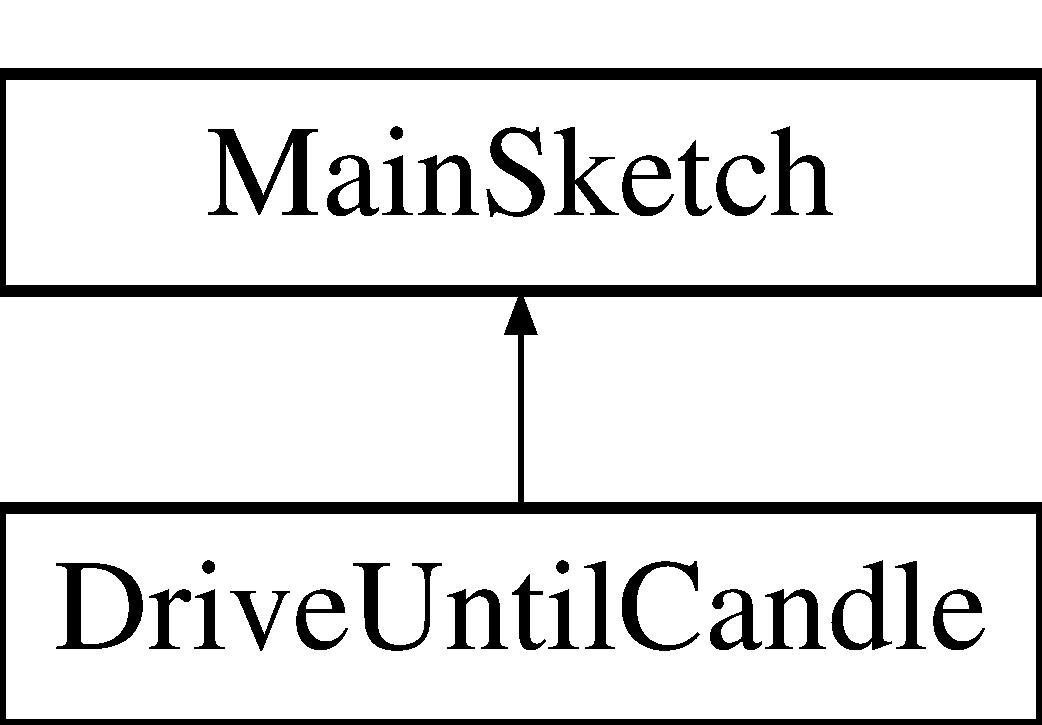
\includegraphics[height=2.000000cm]{classDriveUntilCandle}
\end{center}
\end{figure}
\subsection*{Public Member Functions}
\begin{DoxyCompactItemize}
\item 
void \hyperlink{classDriveUntilCandle_a520ee2277625ce84b594b0a073d23f84}{setup} ()
\item 
void \hyperlink{classDriveUntilCandle_a6c5970d7250b2fd9658bb1a84d2a4ce7}{loop} ()
\item 
void \hyperlink{classDriveUntilCandle_a0d72ef9e0ab6b731b36ecfce2b4fa6f2}{avoid\-In\-Front} (int distance)
\end{DoxyCompactItemize}
\subsection*{Private Attributes}
\begin{DoxyCompactItemize}
\item 
\hyperlink{classLidar}{Lidar} \hyperlink{classDriveUntilCandle_a483790cb5a28465c04fd6c42374d85ac}{lidar}
\item 
\hyperlink{classPIDBase}{P\-I\-D\-Base} \hyperlink{classDriveUntilCandle_a22ecc867ba274ca665b71a6f762b7873}{base}
\item 
int $\ast$ \hyperlink{classDriveUntilCandle_ab1308b79db403f3c35b2d84b8254c349}{distances}
\item 
bool \hyperlink{classDriveUntilCandle_a99cfadc7663aebef445e59d721dfe0bc}{found\-Candle}
\item 
bool \hyperlink{classDriveUntilCandle_a4a3766796623146b80c0a3fa083136d3}{considering\-Candle}
\item 
\hyperlink{classCandleDetector}{Candle\-Detector} \hyperlink{classDriveUntilCandle_af93647db50bc410773c8399642b91450}{cd}
\item 
int \hyperlink{classDriveUntilCandle_a786f5c46c30956d8fafdd57f143b4960}{candle\-Angle} = 0
\item 
int \hyperlink{classDriveUntilCandle_a36b2ce9badf48a77df0ce3ecd38922ec}{candle\-Distance} = 0
\item 
int \hyperlink{classDriveUntilCandle_a518d428f126c93f016e62c8b1ac88c2f}{count} = 0
\end{DoxyCompactItemize}


\subsection{Detailed Description}


Definition at line 7 of file Drive\-Until\-Candle.\-hpp.



\subsection{Member Function Documentation}
\hypertarget{classDriveUntilCandle_a0d72ef9e0ab6b731b36ecfce2b4fa6f2}{\index{Drive\-Until\-Candle@{Drive\-Until\-Candle}!avoid\-In\-Front@{avoid\-In\-Front}}
\index{avoid\-In\-Front@{avoid\-In\-Front}!DriveUntilCandle@{Drive\-Until\-Candle}}
\subsubsection[{avoid\-In\-Front}]{\setlength{\rightskip}{0pt plus 5cm}void Drive\-Until\-Candle\-::avoid\-In\-Front (
\begin{DoxyParamCaption}
\item[{int}]{distance}
\end{DoxyParamCaption}
)}}\label{classDriveUntilCandle_a0d72ef9e0ab6b731b36ecfce2b4fa6f2}


Definition at line 11 of file Drive\-Until\-Candle.\-cpp.

\hypertarget{classDriveUntilCandle_a6c5970d7250b2fd9658bb1a84d2a4ce7}{\index{Drive\-Until\-Candle@{Drive\-Until\-Candle}!loop@{loop}}
\index{loop@{loop}!DriveUntilCandle@{Drive\-Until\-Candle}}
\subsubsection[{loop}]{\setlength{\rightskip}{0pt plus 5cm}void Drive\-Until\-Candle\-::loop (
\begin{DoxyParamCaption}
{}
\end{DoxyParamCaption}
)\hspace{0.3cm}{\ttfamily [virtual]}}}\label{classDriveUntilCandle_a6c5970d7250b2fd9658bb1a84d2a4ce7}


Implements \hyperlink{classMainSketch_acd69845de8c794dce73d309f142a6795}{Main\-Sketch}.



Definition at line 20 of file Drive\-Until\-Candle.\-cpp.

\hypertarget{classDriveUntilCandle_a520ee2277625ce84b594b0a073d23f84}{\index{Drive\-Until\-Candle@{Drive\-Until\-Candle}!setup@{setup}}
\index{setup@{setup}!DriveUntilCandle@{Drive\-Until\-Candle}}
\subsubsection[{setup}]{\setlength{\rightskip}{0pt plus 5cm}void Drive\-Until\-Candle\-::setup (
\begin{DoxyParamCaption}
{}
\end{DoxyParamCaption}
)\hspace{0.3cm}{\ttfamily [virtual]}}}\label{classDriveUntilCandle_a520ee2277625ce84b594b0a073d23f84}


Implements \hyperlink{classMainSketch_a0708e1eb0ced1063f600f4111df90bf2}{Main\-Sketch}.



Definition at line 5 of file Drive\-Until\-Candle.\-cpp.



\subsection{Member Data Documentation}
\hypertarget{classDriveUntilCandle_a22ecc867ba274ca665b71a6f762b7873}{\index{Drive\-Until\-Candle@{Drive\-Until\-Candle}!base@{base}}
\index{base@{base}!DriveUntilCandle@{Drive\-Until\-Candle}}
\subsubsection[{base}]{\setlength{\rightskip}{0pt plus 5cm}{\bf P\-I\-D\-Base} Drive\-Until\-Candle\-::base\hspace{0.3cm}{\ttfamily [private]}}}\label{classDriveUntilCandle_a22ecc867ba274ca665b71a6f762b7873}


Definition at line 16 of file Drive\-Until\-Candle.\-hpp.

\hypertarget{classDriveUntilCandle_a786f5c46c30956d8fafdd57f143b4960}{\index{Drive\-Until\-Candle@{Drive\-Until\-Candle}!candle\-Angle@{candle\-Angle}}
\index{candle\-Angle@{candle\-Angle}!DriveUntilCandle@{Drive\-Until\-Candle}}
\subsubsection[{candle\-Angle}]{\setlength{\rightskip}{0pt plus 5cm}int Drive\-Until\-Candle\-::candle\-Angle = 0\hspace{0.3cm}{\ttfamily [private]}}}\label{classDriveUntilCandle_a786f5c46c30956d8fafdd57f143b4960}


Definition at line 21 of file Drive\-Until\-Candle.\-hpp.

\hypertarget{classDriveUntilCandle_a36b2ce9badf48a77df0ce3ecd38922ec}{\index{Drive\-Until\-Candle@{Drive\-Until\-Candle}!candle\-Distance@{candle\-Distance}}
\index{candle\-Distance@{candle\-Distance}!DriveUntilCandle@{Drive\-Until\-Candle}}
\subsubsection[{candle\-Distance}]{\setlength{\rightskip}{0pt plus 5cm}int Drive\-Until\-Candle\-::candle\-Distance = 0\hspace{0.3cm}{\ttfamily [private]}}}\label{classDriveUntilCandle_a36b2ce9badf48a77df0ce3ecd38922ec}


Definition at line 22 of file Drive\-Until\-Candle.\-hpp.

\hypertarget{classDriveUntilCandle_af93647db50bc410773c8399642b91450}{\index{Drive\-Until\-Candle@{Drive\-Until\-Candle}!cd@{cd}}
\index{cd@{cd}!DriveUntilCandle@{Drive\-Until\-Candle}}
\subsubsection[{cd}]{\setlength{\rightskip}{0pt plus 5cm}{\bf Candle\-Detector} Drive\-Until\-Candle\-::cd\hspace{0.3cm}{\ttfamily [private]}}}\label{classDriveUntilCandle_af93647db50bc410773c8399642b91450}


Definition at line 20 of file Drive\-Until\-Candle.\-hpp.

\hypertarget{classDriveUntilCandle_a4a3766796623146b80c0a3fa083136d3}{\index{Drive\-Until\-Candle@{Drive\-Until\-Candle}!considering\-Candle@{considering\-Candle}}
\index{considering\-Candle@{considering\-Candle}!DriveUntilCandle@{Drive\-Until\-Candle}}
\subsubsection[{considering\-Candle}]{\setlength{\rightskip}{0pt plus 5cm}bool Drive\-Until\-Candle\-::considering\-Candle\hspace{0.3cm}{\ttfamily [private]}}}\label{classDriveUntilCandle_a4a3766796623146b80c0a3fa083136d3}


Definition at line 18 of file Drive\-Until\-Candle.\-hpp.

\hypertarget{classDriveUntilCandle_a518d428f126c93f016e62c8b1ac88c2f}{\index{Drive\-Until\-Candle@{Drive\-Until\-Candle}!count@{count}}
\index{count@{count}!DriveUntilCandle@{Drive\-Until\-Candle}}
\subsubsection[{count}]{\setlength{\rightskip}{0pt plus 5cm}int Drive\-Until\-Candle\-::count = 0\hspace{0.3cm}{\ttfamily [private]}}}\label{classDriveUntilCandle_a518d428f126c93f016e62c8b1ac88c2f}


Definition at line 23 of file Drive\-Until\-Candle.\-hpp.

\hypertarget{classDriveUntilCandle_ab1308b79db403f3c35b2d84b8254c349}{\index{Drive\-Until\-Candle@{Drive\-Until\-Candle}!distances@{distances}}
\index{distances@{distances}!DriveUntilCandle@{Drive\-Until\-Candle}}
\subsubsection[{distances}]{\setlength{\rightskip}{0pt plus 5cm}int$\ast$ Drive\-Until\-Candle\-::distances\hspace{0.3cm}{\ttfamily [private]}}}\label{classDriveUntilCandle_ab1308b79db403f3c35b2d84b8254c349}


Definition at line 17 of file Drive\-Until\-Candle.\-hpp.

\hypertarget{classDriveUntilCandle_a99cfadc7663aebef445e59d721dfe0bc}{\index{Drive\-Until\-Candle@{Drive\-Until\-Candle}!found\-Candle@{found\-Candle}}
\index{found\-Candle@{found\-Candle}!DriveUntilCandle@{Drive\-Until\-Candle}}
\subsubsection[{found\-Candle}]{\setlength{\rightskip}{0pt plus 5cm}bool Drive\-Until\-Candle\-::found\-Candle\hspace{0.3cm}{\ttfamily [private]}}}\label{classDriveUntilCandle_a99cfadc7663aebef445e59d721dfe0bc}


Definition at line 18 of file Drive\-Until\-Candle.\-hpp.

\hypertarget{classDriveUntilCandle_a483790cb5a28465c04fd6c42374d85ac}{\index{Drive\-Until\-Candle@{Drive\-Until\-Candle}!lidar@{lidar}}
\index{lidar@{lidar}!DriveUntilCandle@{Drive\-Until\-Candle}}
\subsubsection[{lidar}]{\setlength{\rightskip}{0pt plus 5cm}{\bf Lidar} Drive\-Until\-Candle\-::lidar\hspace{0.3cm}{\ttfamily [private]}}}\label{classDriveUntilCandle_a483790cb5a28465c04fd6c42374d85ac}


Definition at line 15 of file Drive\-Until\-Candle.\-hpp.



The documentation for this class was generated from the following files\-:\begin{DoxyCompactItemize}
\item 
src/test/\hyperlink{DriveUntilCandle_8hpp}{Drive\-Until\-Candle.\-hpp}\item 
src/test/\hyperlink{DriveUntilCandle_8cpp}{Drive\-Until\-Candle.\-cpp}\end{DoxyCompactItemize}

\hypertarget{classEncoder}{\section{Encoder$<$ port1, port2 $>$ Class Template Reference}
\label{classEncoder}\index{Encoder$<$ port1, port2 $>$@{Encoder$<$ port1, port2 $>$}}
}


{\ttfamily \#include $<$Encoder.\-hpp$>$}

\subsection*{Static Public Member Functions}
\begin{DoxyCompactItemize}
\item 
static void \hyperlink{classEncoder_a7945aef1fa1eef9c69eae3059c7383f5}{setup} ()
\item 
static int \hyperlink{classEncoder_ad4a82c2cb43afce3149e206e42796173}{read} (bool reset=false)
\end{DoxyCompactItemize}
\subsection*{Static Private Member Functions}
\begin{DoxyCompactItemize}
\item 
static void \hyperlink{classEncoder_ac4291694602efae2fd808c622aa08466}{isr\-\_\-a} ()
\item 
static void \hyperlink{classEncoder_a13da10ca35269f3e369c637e3fe492e9}{isr\-\_\-b} ()
\end{DoxyCompactItemize}
\subsection*{Static Private Attributes}
\begin{DoxyCompactItemize}
\item 
static int \hyperlink{classEncoder_af68226c82a0ec90d00cc40d733ca9eab}{last\-\_\-a} = 0
\item 
static int \hyperlink{classEncoder_a5a4bc2fcd23a97e69a47ecf3cd6e0914}{last\-\_\-b} = 0
\item 
static int \hyperlink{classEncoder_a7f71986ee5780e0fe3a91c93b7116c38}{count} = 0
\end{DoxyCompactItemize}


\subsection{Detailed Description}
\subsubsection*{template$<$int port1, int port2$>$class Encoder$<$ port1, port2 $>$}



Definition at line 5 of file Encoder.\-hpp.



\subsection{Member Function Documentation}
\hypertarget{classEncoder_ac4291694602efae2fd808c622aa08466}{\index{Encoder@{Encoder}!isr\-\_\-a@{isr\-\_\-a}}
\index{isr\-\_\-a@{isr\-\_\-a}!Encoder@{Encoder}}
\subsubsection[{isr\-\_\-a}]{\setlength{\rightskip}{0pt plus 5cm}template$<$int port1, int port2$>$ static void {\bf Encoder}$<$ port1, port2 $>$\-::isr\-\_\-a (
\begin{DoxyParamCaption}
{}
\end{DoxyParamCaption}
)\hspace{0.3cm}{\ttfamily [inline]}, {\ttfamily [static]}, {\ttfamily [private]}}}\label{classEncoder_ac4291694602efae2fd808c622aa08466}


Definition at line 23 of file Encoder.\-hpp.

\hypertarget{classEncoder_a13da10ca35269f3e369c637e3fe492e9}{\index{Encoder@{Encoder}!isr\-\_\-b@{isr\-\_\-b}}
\index{isr\-\_\-b@{isr\-\_\-b}!Encoder@{Encoder}}
\subsubsection[{isr\-\_\-b}]{\setlength{\rightskip}{0pt plus 5cm}template$<$int port1, int port2$>$ static void {\bf Encoder}$<$ port1, port2 $>$\-::isr\-\_\-b (
\begin{DoxyParamCaption}
{}
\end{DoxyParamCaption}
)\hspace{0.3cm}{\ttfamily [inline]}, {\ttfamily [static]}, {\ttfamily [private]}}}\label{classEncoder_a13da10ca35269f3e369c637e3fe492e9}


Definition at line 41 of file Encoder.\-hpp.

\hypertarget{classEncoder_ad4a82c2cb43afce3149e206e42796173}{\index{Encoder@{Encoder}!read@{read}}
\index{read@{read}!Encoder@{Encoder}}
\subsubsection[{read}]{\setlength{\rightskip}{0pt plus 5cm}template$<$int port1, int port2$>$ static int {\bf Encoder}$<$ port1, port2 $>$\-::read (
\begin{DoxyParamCaption}
\item[{bool}]{reset = {\ttfamily false}}
\end{DoxyParamCaption}
)\hspace{0.3cm}{\ttfamily [inline]}, {\ttfamily [static]}}}\label{classEncoder_ad4a82c2cb43afce3149e206e42796173}


Definition at line 17 of file Encoder.\-hpp.

\hypertarget{classEncoder_a7945aef1fa1eef9c69eae3059c7383f5}{\index{Encoder@{Encoder}!setup@{setup}}
\index{setup@{setup}!Encoder@{Encoder}}
\subsubsection[{setup}]{\setlength{\rightskip}{0pt plus 5cm}template$<$int port1, int port2$>$ static void {\bf Encoder}$<$ port1, port2 $>$\-::setup (
\begin{DoxyParamCaption}
{}
\end{DoxyParamCaption}
)\hspace{0.3cm}{\ttfamily [inline]}, {\ttfamily [static]}}}\label{classEncoder_a7945aef1fa1eef9c69eae3059c7383f5}


Definition at line 7 of file Encoder.\-hpp.



\subsection{Member Data Documentation}
\hypertarget{classEncoder_a7f71986ee5780e0fe3a91c93b7116c38}{\index{Encoder@{Encoder}!count@{count}}
\index{count@{count}!Encoder@{Encoder}}
\subsubsection[{count}]{\setlength{\rightskip}{0pt plus 5cm}template$<$int port1, int port2$>$ int {\bf Encoder}$<$ a, b $>$\-::count = 0\hspace{0.3cm}{\ttfamily [static]}, {\ttfamily [private]}}}\label{classEncoder_a7f71986ee5780e0fe3a91c93b7116c38}


Definition at line 61 of file Encoder.\-hpp.

\hypertarget{classEncoder_af68226c82a0ec90d00cc40d733ca9eab}{\index{Encoder@{Encoder}!last\-\_\-a@{last\-\_\-a}}
\index{last\-\_\-a@{last\-\_\-a}!Encoder@{Encoder}}
\subsubsection[{last\-\_\-a}]{\setlength{\rightskip}{0pt plus 5cm}template$<$int port1, int port2$>$ int {\bf Encoder}$<$ a, b $>$\-::last\-\_\-a = 0\hspace{0.3cm}{\ttfamily [static]}, {\ttfamily [private]}}}\label{classEncoder_af68226c82a0ec90d00cc40d733ca9eab}


Definition at line 59 of file Encoder.\-hpp.

\hypertarget{classEncoder_a5a4bc2fcd23a97e69a47ecf3cd6e0914}{\index{Encoder@{Encoder}!last\-\_\-b@{last\-\_\-b}}
\index{last\-\_\-b@{last\-\_\-b}!Encoder@{Encoder}}
\subsubsection[{last\-\_\-b}]{\setlength{\rightskip}{0pt plus 5cm}template$<$int port1, int port2$>$ int {\bf Encoder}$<$ a, b $>$\-::last\-\_\-b = 0\hspace{0.3cm}{\ttfamily [static]}, {\ttfamily [private]}}}\label{classEncoder_a5a4bc2fcd23a97e69a47ecf3cd6e0914}


Definition at line 60 of file Encoder.\-hpp.



The documentation for this class was generated from the following file\-:\begin{DoxyCompactItemize}
\item 
src/shared/\hyperlink{Encoder_8hpp}{Encoder.\-hpp}\end{DoxyCompactItemize}

\hypertarget{classExtinguisher}{\section{Extinguisher Class Reference}
\label{classExtinguisher}\index{Extinguisher@{Extinguisher}}
}


houses the state machine for extinguishing the candle \hyperlink{classFan}{Fan} is included  




{\ttfamily \#include $<$Extinguisher.\-hpp$>$}

\subsection*{Public Member Functions}
\begin{DoxyCompactItemize}
\item 
void \hyperlink{classExtinguisher_a5a6f4652de68d87d3c94a5133770036f}{setup} ()
\begin{DoxyCompactList}\small\item\em setup fan and state machine. Called my main setup \end{DoxyCompactList}\item 
void \hyperlink{classExtinguisher_add162f2794a81915e50bdde84f582ab9}{change\-State} (\hyperlink{classExtinguisher_a969a7cce3382fc5d67f687540896e3ab}{State} \hyperlink{classExtinguisher_aa67c13dc091e5dc2c054d53f7fcae69b}{state})
\item 
bool \hyperlink{classExtinguisher_ab11afd0f55af4485a1a4f369c7743a40}{run} ()
\begin{DoxyCompactList}\small\item\em state machine method. States liste in $\ast$state\-Names \end{DoxyCompactList}\end{DoxyCompactItemize}
\subsection*{Private Types}
\begin{DoxyCompactItemize}
\item 
enum \hyperlink{classExtinguisher_a969a7cce3382fc5d67f687540896e3ab}{State} \{ \\*
\hyperlink{classExtinguisher_a969a7cce3382fc5d67f687540896e3aba25f6661e71a4e779393f9e1d0afdb9cd}{I\-N\-I\-T}, 
\hyperlink{classExtinguisher_a969a7cce3382fc5d67f687540896e3aba2ff965592f07601418ca89485f335cb2}{T\-U\-R\-N\-I\-N\-G\-\_\-\-T\-O\-\_\-\-B\-L\-O\-W}, 
\hyperlink{classExtinguisher_a969a7cce3382fc5d67f687540896e3aba1defb0b77459569c811478b71cbbf13e}{T\-U\-R\-N\-I\-N\-G\-\_\-\-T\-O\-\_\-\-V\-E\-R\-I\-F\-Y}, 
\hyperlink{classExtinguisher_a969a7cce3382fc5d67f687540896e3aba9d3fa0261c6cf909a97ca68eee27ed0d}{B\-L\-O\-W\-I\-N\-G}, 
\\*
\hyperlink{classExtinguisher_a969a7cce3382fc5d67f687540896e3aba5152bb2f7b6f5f9f8b53204d0ae61ddd}{V\-E\-R\-I\-F\-Y\-I\-N\-G}
 \}
\end{DoxyCompactItemize}
\subsection*{Private Attributes}
\begin{DoxyCompactItemize}
\item 
\hyperlink{classFan}{Fan} \hyperlink{classExtinguisher_a47ec6f79ddc26b18bbc1a0ac9741ae24}{fan}
\begin{DoxyCompactList}\small\item\em Extinguishing fan. \end{DoxyCompactList}\item 
\hyperlink{classExtinguisher_a969a7cce3382fc5d67f687540896e3ab}{State} \hyperlink{classExtinguisher_aa67c13dc091e5dc2c054d53f7fcae69b}{state}
\begin{DoxyCompactList}\small\item\em State Machine control variable. \end{DoxyCompactList}\item 
long \hyperlink{classExtinguisher_a75020779b6ba6fcd9ac11148a378d441}{start\-State\-Time} = 0l
\begin{DoxyCompactList}\small\item\em Timer variable for time based states. \end{DoxyCompactList}\item 
float \hyperlink{classExtinguisher_af7b156761cc23a5bee07f3cecd50213a}{goal\-Angle} = 0.\-0f
\begin{DoxyCompactList}\small\item\em Goal Angle to face after turns. \end{DoxyCompactList}\item 
const char $\ast$ \hyperlink{classExtinguisher_a91cd54af9125620a68939ccdc5796c66}{state\-Names} \mbox{[}5\mbox{]}
\begin{DoxyCompactList}\small\item\em Names of States. \end{DoxyCompactList}\end{DoxyCompactItemize}
\subsection*{Static Private Attributes}
\begin{DoxyCompactItemize}
\item 
static const int \hyperlink{classExtinguisher_a454a63d5013db7cec4e5ae18fbfe64fa}{B\-L\-O\-W\-\_\-\-T\-I\-M\-E} = 6000
\begin{DoxyCompactList}\small\item\em Length of timers. \end{DoxyCompactList}\item 
static const int \hyperlink{classExtinguisher_a1f4f2c248d5fcf98a62eab8019ab79f9}{V\-E\-R\-I\-F\-Y\-\_\-\-T\-I\-M\-E} = 2000
\end{DoxyCompactItemize}


\subsection{Detailed Description}
houses the state machine for extinguishing the candle \hyperlink{classFan}{Fan} is included 

Definition at line 8 of file Extinguisher.\-hpp.



\subsection{Member Enumeration Documentation}
\hypertarget{classExtinguisher_a969a7cce3382fc5d67f687540896e3ab}{\index{Extinguisher@{Extinguisher}!State@{State}}
\index{State@{State}!Extinguisher@{Extinguisher}}
\subsubsection[{State}]{\setlength{\rightskip}{0pt plus 5cm}enum {\bf Extinguisher\-::\-State}\hspace{0.3cm}{\ttfamily [private]}}}\label{classExtinguisher_a969a7cce3382fc5d67f687540896e3ab}
\begin{Desc}
\item[Enumerator]\par
\begin{description}
\index{I\-N\-I\-T@{I\-N\-I\-T}!Extinguisher@{Extinguisher}}\index{Extinguisher@{Extinguisher}!I\-N\-I\-T@{I\-N\-I\-T}}\item[{\em 
\hypertarget{classExtinguisher_a969a7cce3382fc5d67f687540896e3aba25f6661e71a4e779393f9e1d0afdb9cd}{I\-N\-I\-T}\label{classExtinguisher_a969a7cce3382fc5d67f687540896e3aba25f6661e71a4e779393f9e1d0afdb9cd}
}]\index{T\-U\-R\-N\-I\-N\-G\-\_\-\-T\-O\-\_\-\-B\-L\-O\-W@{T\-U\-R\-N\-I\-N\-G\-\_\-\-T\-O\-\_\-\-B\-L\-O\-W}!Extinguisher@{Extinguisher}}\index{Extinguisher@{Extinguisher}!T\-U\-R\-N\-I\-N\-G\-\_\-\-T\-O\-\_\-\-B\-L\-O\-W@{T\-U\-R\-N\-I\-N\-G\-\_\-\-T\-O\-\_\-\-B\-L\-O\-W}}\item[{\em 
\hypertarget{classExtinguisher_a969a7cce3382fc5d67f687540896e3aba2ff965592f07601418ca89485f335cb2}{T\-U\-R\-N\-I\-N\-G\-\_\-\-T\-O\-\_\-\-B\-L\-O\-W}\label{classExtinguisher_a969a7cce3382fc5d67f687540896e3aba2ff965592f07601418ca89485f335cb2}
}]\index{T\-U\-R\-N\-I\-N\-G\-\_\-\-T\-O\-\_\-\-V\-E\-R\-I\-F\-Y@{T\-U\-R\-N\-I\-N\-G\-\_\-\-T\-O\-\_\-\-V\-E\-R\-I\-F\-Y}!Extinguisher@{Extinguisher}}\index{Extinguisher@{Extinguisher}!T\-U\-R\-N\-I\-N\-G\-\_\-\-T\-O\-\_\-\-V\-E\-R\-I\-F\-Y@{T\-U\-R\-N\-I\-N\-G\-\_\-\-T\-O\-\_\-\-V\-E\-R\-I\-F\-Y}}\item[{\em 
\hypertarget{classExtinguisher_a969a7cce3382fc5d67f687540896e3aba1defb0b77459569c811478b71cbbf13e}{T\-U\-R\-N\-I\-N\-G\-\_\-\-T\-O\-\_\-\-V\-E\-R\-I\-F\-Y}\label{classExtinguisher_a969a7cce3382fc5d67f687540896e3aba1defb0b77459569c811478b71cbbf13e}
}]\index{B\-L\-O\-W\-I\-N\-G@{B\-L\-O\-W\-I\-N\-G}!Extinguisher@{Extinguisher}}\index{Extinguisher@{Extinguisher}!B\-L\-O\-W\-I\-N\-G@{B\-L\-O\-W\-I\-N\-G}}\item[{\em 
\hypertarget{classExtinguisher_a969a7cce3382fc5d67f687540896e3aba9d3fa0261c6cf909a97ca68eee27ed0d}{B\-L\-O\-W\-I\-N\-G}\label{classExtinguisher_a969a7cce3382fc5d67f687540896e3aba9d3fa0261c6cf909a97ca68eee27ed0d}
}]\index{V\-E\-R\-I\-F\-Y\-I\-N\-G@{V\-E\-R\-I\-F\-Y\-I\-N\-G}!Extinguisher@{Extinguisher}}\index{Extinguisher@{Extinguisher}!V\-E\-R\-I\-F\-Y\-I\-N\-G@{V\-E\-R\-I\-F\-Y\-I\-N\-G}}\item[{\em 
\hypertarget{classExtinguisher_a969a7cce3382fc5d67f687540896e3aba5152bb2f7b6f5f9f8b53204d0ae61ddd}{V\-E\-R\-I\-F\-Y\-I\-N\-G}\label{classExtinguisher_a969a7cce3382fc5d67f687540896e3aba5152bb2f7b6f5f9f8b53204d0ae61ddd}
}]\end{description}
\end{Desc}


Definition at line 10 of file Extinguisher.\-hpp.



\subsection{Member Function Documentation}
\hypertarget{classExtinguisher_add162f2794a81915e50bdde84f582ab9}{\index{Extinguisher@{Extinguisher}!change\-State@{change\-State}}
\index{change\-State@{change\-State}!Extinguisher@{Extinguisher}}
\subsubsection[{change\-State}]{\setlength{\rightskip}{0pt plus 5cm}void Extinguisher\-::change\-State (
\begin{DoxyParamCaption}
\item[{{\bf State}}]{state}
\end{DoxyParamCaption}
)}}\label{classExtinguisher_add162f2794a81915e50bdde84f582ab9}


Definition at line 10 of file Extinguisher.\-cpp.

\hypertarget{classExtinguisher_ab11afd0f55af4485a1a4f369c7743a40}{\index{Extinguisher@{Extinguisher}!run@{run}}
\index{run@{run}!Extinguisher@{Extinguisher}}
\subsubsection[{run}]{\setlength{\rightskip}{0pt plus 5cm}bool Extinguisher\-::run (
\begin{DoxyParamCaption}
{}
\end{DoxyParamCaption}
)}}\label{classExtinguisher_ab11afd0f55af4485a1a4f369c7743a40}


state machine method. States liste in $\ast$state\-Names 



Definition at line 15 of file Extinguisher.\-cpp.

\hypertarget{classExtinguisher_a5a6f4652de68d87d3c94a5133770036f}{\index{Extinguisher@{Extinguisher}!setup@{setup}}
\index{setup@{setup}!Extinguisher@{Extinguisher}}
\subsubsection[{setup}]{\setlength{\rightskip}{0pt plus 5cm}void Extinguisher\-::setup (
\begin{DoxyParamCaption}
{}
\end{DoxyParamCaption}
)}}\label{classExtinguisher_a5a6f4652de68d87d3c94a5133770036f}


setup fan and state machine. Called my main setup 



Definition at line 5 of file Extinguisher.\-cpp.



\subsection{Member Data Documentation}
\hypertarget{classExtinguisher_a454a63d5013db7cec4e5ae18fbfe64fa}{\index{Extinguisher@{Extinguisher}!B\-L\-O\-W\-\_\-\-T\-I\-M\-E@{B\-L\-O\-W\-\_\-\-T\-I\-M\-E}}
\index{B\-L\-O\-W\-\_\-\-T\-I\-M\-E@{B\-L\-O\-W\-\_\-\-T\-I\-M\-E}!Extinguisher@{Extinguisher}}
\subsubsection[{B\-L\-O\-W\-\_\-\-T\-I\-M\-E}]{\setlength{\rightskip}{0pt plus 5cm}const int Extinguisher\-::\-B\-L\-O\-W\-\_\-\-T\-I\-M\-E = 6000\hspace{0.3cm}{\ttfamily [static]}, {\ttfamily [private]}}}\label{classExtinguisher_a454a63d5013db7cec4e5ae18fbfe64fa}


Length of timers. 



Definition at line 41 of file Extinguisher.\-hpp.

\hypertarget{classExtinguisher_a47ec6f79ddc26b18bbc1a0ac9741ae24}{\index{Extinguisher@{Extinguisher}!fan@{fan}}
\index{fan@{fan}!Extinguisher@{Extinguisher}}
\subsubsection[{fan}]{\setlength{\rightskip}{0pt plus 5cm}{\bf Fan} Extinguisher\-::fan\hspace{0.3cm}{\ttfamily [private]}}}\label{classExtinguisher_a47ec6f79ddc26b18bbc1a0ac9741ae24}


Extinguishing fan. 



Definition at line 29 of file Extinguisher.\-hpp.

\hypertarget{classExtinguisher_af7b156761cc23a5bee07f3cecd50213a}{\index{Extinguisher@{Extinguisher}!goal\-Angle@{goal\-Angle}}
\index{goal\-Angle@{goal\-Angle}!Extinguisher@{Extinguisher}}
\subsubsection[{goal\-Angle}]{\setlength{\rightskip}{0pt plus 5cm}float Extinguisher\-::goal\-Angle = 0.\-0f\hspace{0.3cm}{\ttfamily [private]}}}\label{classExtinguisher_af7b156761cc23a5bee07f3cecd50213a}


Goal Angle to face after turns. 



Definition at line 38 of file Extinguisher.\-hpp.

\hypertarget{classExtinguisher_a75020779b6ba6fcd9ac11148a378d441}{\index{Extinguisher@{Extinguisher}!start\-State\-Time@{start\-State\-Time}}
\index{start\-State\-Time@{start\-State\-Time}!Extinguisher@{Extinguisher}}
\subsubsection[{start\-State\-Time}]{\setlength{\rightskip}{0pt plus 5cm}long Extinguisher\-::start\-State\-Time = 0l\hspace{0.3cm}{\ttfamily [private]}}}\label{classExtinguisher_a75020779b6ba6fcd9ac11148a378d441}


Timer variable for time based states. 



Definition at line 35 of file Extinguisher.\-hpp.

\hypertarget{classExtinguisher_aa67c13dc091e5dc2c054d53f7fcae69b}{\index{Extinguisher@{Extinguisher}!state@{state}}
\index{state@{state}!Extinguisher@{Extinguisher}}
\subsubsection[{state}]{\setlength{\rightskip}{0pt plus 5cm}{\bf State} Extinguisher\-::state\hspace{0.3cm}{\ttfamily [private]}}}\label{classExtinguisher_aa67c13dc091e5dc2c054d53f7fcae69b}


State Machine control variable. 



Definition at line 32 of file Extinguisher.\-hpp.

\hypertarget{classExtinguisher_a91cd54af9125620a68939ccdc5796c66}{\index{Extinguisher@{Extinguisher}!state\-Names@{state\-Names}}
\index{state\-Names@{state\-Names}!Extinguisher@{Extinguisher}}
\subsubsection[{state\-Names}]{\setlength{\rightskip}{0pt plus 5cm}const char$\ast$ Extinguisher\-::state\-Names\mbox{[}5\mbox{]}\hspace{0.3cm}{\ttfamily [private]}}}\label{classExtinguisher_a91cd54af9125620a68939ccdc5796c66}
{\bfseries Initial value\-:}
\begin{DoxyCode}
= \{
      \textcolor{stringliteral}{"INIT          "},
      \textcolor{stringliteral}{"TURNING\_BLOW  "},
      \textcolor{stringliteral}{"TURNING\_VERIFY"},
      \textcolor{stringliteral}{"BLOWING       "},
      \textcolor{stringliteral}{"VERIFYING     "}\}
\end{DoxyCode}


Names of States. 



Definition at line 45 of file Extinguisher.\-hpp.

\hypertarget{classExtinguisher_a1f4f2c248d5fcf98a62eab8019ab79f9}{\index{Extinguisher@{Extinguisher}!V\-E\-R\-I\-F\-Y\-\_\-\-T\-I\-M\-E@{V\-E\-R\-I\-F\-Y\-\_\-\-T\-I\-M\-E}}
\index{V\-E\-R\-I\-F\-Y\-\_\-\-T\-I\-M\-E@{V\-E\-R\-I\-F\-Y\-\_\-\-T\-I\-M\-E}!Extinguisher@{Extinguisher}}
\subsubsection[{V\-E\-R\-I\-F\-Y\-\_\-\-T\-I\-M\-E}]{\setlength{\rightskip}{0pt plus 5cm}const int Extinguisher\-::\-V\-E\-R\-I\-F\-Y\-\_\-\-T\-I\-M\-E = 2000\hspace{0.3cm}{\ttfamily [static]}, {\ttfamily [private]}}}\label{classExtinguisher_a1f4f2c248d5fcf98a62eab8019ab79f9}


Definition at line 42 of file Extinguisher.\-hpp.



The documentation for this class was generated from the following files\-:\begin{DoxyCompactItemize}
\item 
src/shared/\hyperlink{Extinguisher_8hpp}{Extinguisher.\-hpp}\item 
src/shared/\hyperlink{Extinguisher_8cpp}{Extinguisher.\-cpp}\end{DoxyCompactItemize}

\hypertarget{classFan}{\section{Fan Class Reference}
\label{classFan}\index{Fan@{Fan}}
}


Wrapper around Servo the control 1000\-K\-V Outrunner.  




{\ttfamily \#include $<$Fan.\-hpp$>$}

\subsection*{Public Member Functions}
\begin{DoxyCompactItemize}
\item 
void \hyperlink{classFan_afa6c28ec10c0f00270e04abc8344e220}{setup} ()
\begin{DoxyCompactList}\small\item\em Setup for the servo object. Also handles arming of the E\-S\-C. \end{DoxyCompactList}\item 
void \hyperlink{classFan_ab0574452a1e4ad34f668b4792be6021c}{spin} ()
\begin{DoxyCompactList}\small\item\em spin the motor at F\-U\-L\-L P\-O\-W\-E\-R! \end{DoxyCompactList}\item 
void \hyperlink{classFan_af4a96b6fd535b30f933a8bf8d1af50ff}{stop} ()
\begin{DoxyCompactList}\small\item\em stop the motor. speed controller will ramp it down for us \end{DoxyCompactList}\end{DoxyCompactItemize}
\subsection*{Private Attributes}
\begin{DoxyCompactItemize}
\item 
Servo \hyperlink{classFan_aff9de16d110a96ff5788f7d6ad6ef715}{motor}
\begin{DoxyCompactList}\small\item\em internal motor object \end{DoxyCompactList}\end{DoxyCompactItemize}
\subsection*{Static Private Attributes}
\begin{DoxyCompactItemize}
\item 
static const int \hyperlink{classFan_a8d7eb0f5de190ffc2f5d0ae1c5c10e29}{I\-N\-I\-T\-\_\-\-P\-A\-U\-S\-E} = 3000
\begin{DoxyCompactList}\small\item\em the pause time between E\-S\-C arming sequences \end{DoxyCompactList}\end{DoxyCompactItemize}


\subsection{Detailed Description}
Wrapper around Servo the control 1000\-K\-V Outrunner. 

Definition at line 8 of file Fan.\-hpp.



\subsection{Member Function Documentation}
\hypertarget{classFan_afa6c28ec10c0f00270e04abc8344e220}{\index{Fan@{Fan}!setup@{setup}}
\index{setup@{setup}!Fan@{Fan}}
\subsubsection[{setup}]{\setlength{\rightskip}{0pt plus 5cm}void Fan\-::setup (
\begin{DoxyParamCaption}
{}
\end{DoxyParamCaption}
)}}\label{classFan_afa6c28ec10c0f00270e04abc8344e220}


Setup for the servo object. Also handles arming of the E\-S\-C. 



Definition at line 4 of file Fan.\-cpp.

\hypertarget{classFan_ab0574452a1e4ad34f668b4792be6021c}{\index{Fan@{Fan}!spin@{spin}}
\index{spin@{spin}!Fan@{Fan}}
\subsubsection[{spin}]{\setlength{\rightskip}{0pt plus 5cm}void Fan\-::spin (
\begin{DoxyParamCaption}
{}
\end{DoxyParamCaption}
)}}\label{classFan_ab0574452a1e4ad34f668b4792be6021c}


spin the motor at F\-U\-L\-L P\-O\-W\-E\-R! 



Definition at line 12 of file Fan.\-cpp.

\hypertarget{classFan_af4a96b6fd535b30f933a8bf8d1af50ff}{\index{Fan@{Fan}!stop@{stop}}
\index{stop@{stop}!Fan@{Fan}}
\subsubsection[{stop}]{\setlength{\rightskip}{0pt plus 5cm}void Fan\-::stop (
\begin{DoxyParamCaption}
{}
\end{DoxyParamCaption}
)}}\label{classFan_af4a96b6fd535b30f933a8bf8d1af50ff}


stop the motor. speed controller will ramp it down for us 



Definition at line 16 of file Fan.\-cpp.



\subsection{Member Data Documentation}
\hypertarget{classFan_a8d7eb0f5de190ffc2f5d0ae1c5c10e29}{\index{Fan@{Fan}!I\-N\-I\-T\-\_\-\-P\-A\-U\-S\-E@{I\-N\-I\-T\-\_\-\-P\-A\-U\-S\-E}}
\index{I\-N\-I\-T\-\_\-\-P\-A\-U\-S\-E@{I\-N\-I\-T\-\_\-\-P\-A\-U\-S\-E}!Fan@{Fan}}
\subsubsection[{I\-N\-I\-T\-\_\-\-P\-A\-U\-S\-E}]{\setlength{\rightskip}{0pt plus 5cm}const int Fan\-::\-I\-N\-I\-T\-\_\-\-P\-A\-U\-S\-E = 3000\hspace{0.3cm}{\ttfamily [static]}, {\ttfamily [private]}}}\label{classFan_a8d7eb0f5de190ffc2f5d0ae1c5c10e29}


the pause time between E\-S\-C arming sequences 



Definition at line 26 of file Fan.\-hpp.

\hypertarget{classFan_aff9de16d110a96ff5788f7d6ad6ef715}{\index{Fan@{Fan}!motor@{motor}}
\index{motor@{motor}!Fan@{Fan}}
\subsubsection[{motor}]{\setlength{\rightskip}{0pt plus 5cm}Servo Fan\-::motor\hspace{0.3cm}{\ttfamily [private]}}}\label{classFan_aff9de16d110a96ff5788f7d6ad6ef715}


internal motor object 



Definition at line 23 of file Fan.\-hpp.



The documentation for this class was generated from the following files\-:\begin{DoxyCompactItemize}
\item 
src/shared/\hyperlink{Fan_8hpp}{Fan.\-hpp}\item 
src/shared/\hyperlink{Fan_8cpp}{Fan.\-cpp}\end{DoxyCompactItemize}

\hypertarget{classFireFinder}{\section{Fire\-Finder Class Reference}
\label{classFireFinder}\index{Fire\-Finder@{Fire\-Finder}}
}


Wrapper around head servo, and contains functions for scanning for fire and reporting candle height.  




{\ttfamily \#include $<$Fire\-Finder.\-hpp$>$}

\subsection*{Public Member Functions}
\begin{DoxyCompactItemize}
\item 
void \hyperlink{classFireFinder_aaa2beb5a87e2d9dbd83c0dee1f4f1ef0}{setup} ()
\begin{DoxyCompactList}\small\item\em setup the head servo \end{DoxyCompactList}\item 
void \hyperlink{classFireFinder_ab2cddefdf1200e176231a601a3a1ede3}{start\-Scan} ()
\begin{DoxyCompactList}\small\item\em sets some flags to start scanning for candle. This doesn't actually do any scanning, you have to be callling watch \end{DoxyCompactList}\item 
bool \hyperlink{classFireFinder_afa2879ee6ace8a6b5e298c4186df6178}{sees\-Candle} ()
\begin{DoxyCompactList}\small\item\em Looks directly in front for a candle by sampling I\-R. \end{DoxyCompactList}\item 
float \hyperlink{classFireFinder_afbdb8a5938750d5091becec74fc1f907}{watch} (int d\-To\-Candle)
\begin{DoxyCompactList}\small\item\em Call this continuously to check candle height. \end{DoxyCompactList}\item 
void \hyperlink{classFireFinder_ad0ce95ec7a5858be9b80a3c103120008}{level\-Head} ()
\begin{DoxyCompactList}\small\item\em Simply set the head to 90 degrees. \end{DoxyCompactList}\end{DoxyCompactItemize}
\subsection*{Private Attributes}
\begin{DoxyCompactItemize}
\item 
Servo \hyperlink{classFireFinder_ac6a7b4e986e63cddb3f010e8909c00f8}{head}
\begin{DoxyCompactList}\small\item\em The motor object. \end{DoxyCompactList}\item 
int \hyperlink{classFireFinder_a7d3912a911843b60de3468588cfe8579}{min\-Intensity} = 1024
\begin{DoxyCompactList}\small\item\em min intensity during scan \end{DoxyCompactList}\item 
int \hyperlink{classFireFinder_ad8be0837d88f10d65b6f8a405f29494a}{min\-Position} = 100
\begin{DoxyCompactList}\small\item\em min position during scan \end{DoxyCompactList}\item 
int \hyperlink{classFireFinder_a40e204a2807939b3195024f14a9278fc}{position} = 0
\begin{DoxyCompactList}\small\item\em Current position of head during scan. \end{DoxyCompactList}\item 
bool \hyperlink{classFireFinder_aec1a3ae4b80847a907898601c64386cb}{scanning} = false
\begin{DoxyCompactList}\small\item\em The current state of the scanning routine. \end{DoxyCompactList}\item 
long \hyperlink{classFireFinder_a97b1a598ddb7886feb4a96a4931cc103}{time\-To\-Change\-Angle} = 0l
\begin{DoxyCompactList}\small\item\em Controls the speed of sweeping. \end{DoxyCompactList}\item 
long \hyperlink{classFireFinder_aaa38192d82bc4120129b72fee61f72f1}{sweep\-Time} = 5000l
\item 
long \hyperlink{classFireFinder_ad482526cf32997919cbc31f61d12065d}{step} = 3
\end{DoxyCompactItemize}
\subsection*{Static Private Attributes}
\begin{DoxyCompactItemize}
\item 
static const int \hyperlink{classFireFinder_ac29b178da56a9347787371708bb62a20}{M\-O\-T\-O\-R\-\_\-\-P\-I\-N} = 10
\item 
static const int \hyperlink{classFireFinder_a5afc5290c8ba58893228414ba5965ed3}{S\-E\-N\-S\-O\-R\-\_\-\-P\-I\-N} = 0
\item 
static const int \hyperlink{classFireFinder_ace5a0c6c6435a4d36377dc94a5f785db}{M\-A\-X\-\_\-\-H\-E\-A\-D\-\_\-\-A\-N\-G\-L\-E} = 20
\item 
static const int \hyperlink{classFireFinder_ac6743699fd08f97088855dc1e87f8dea}{M\-I\-N\-\_\-\-H\-E\-A\-D\-\_\-\-A\-N\-G\-L\-E} = -\/35
\item 
static const int \hyperlink{classFireFinder_a2136ca4e2438b84b0f4f3864697d51b1}{S\-A\-M\-P\-L\-E\-\_\-\-S\-I\-Z\-E} = 10
\item 
static const int \hyperlink{classFireFinder_ab145c886fc3edcc215a5673bf4874b13}{S\-E\-N\-S\-O\-R\-\_\-\-H\-E\-I\-G\-H\-T} = 210
\item 
static const int \hyperlink{classFireFinder_a0b9c6aa9ba75e2900477f94b02b2bb0b}{I\-N\-T\-E\-N\-S\-I\-T\-Y\-\_\-\-T\-H\-R\-E\-S\-H\-O\-L\-D} = 35
\item 
static const int \hyperlink{classFireFinder_aa05ce7d7760ac59ea294df68475dcf05}{M\-I\-N\-\_\-\-I\-N\-T\-E\-N\-S\-I\-T\-Y} = 995
\end{DoxyCompactItemize}


\subsection{Detailed Description}
Wrapper around head servo, and contains functions for scanning for fire and reporting candle height. 

Definition at line 7 of file Fire\-Finder.\-hpp.



\subsection{Member Function Documentation}
\hypertarget{classFireFinder_ad0ce95ec7a5858be9b80a3c103120008}{\index{Fire\-Finder@{Fire\-Finder}!level\-Head@{level\-Head}}
\index{level\-Head@{level\-Head}!FireFinder@{Fire\-Finder}}
\subsubsection[{level\-Head}]{\setlength{\rightskip}{0pt plus 5cm}void Fire\-Finder\-::level\-Head (
\begin{DoxyParamCaption}
{}
\end{DoxyParamCaption}
)}}\label{classFireFinder_ad0ce95ec7a5858be9b80a3c103120008}


Simply set the head to 90 degrees. 



Definition at line 9 of file Fire\-Finder.\-cpp.

\hypertarget{classFireFinder_afa2879ee6ace8a6b5e298c4186df6178}{\index{Fire\-Finder@{Fire\-Finder}!sees\-Candle@{sees\-Candle}}
\index{sees\-Candle@{sees\-Candle}!FireFinder@{Fire\-Finder}}
\subsubsection[{sees\-Candle}]{\setlength{\rightskip}{0pt plus 5cm}bool Fire\-Finder\-::sees\-Candle (
\begin{DoxyParamCaption}
{}
\end{DoxyParamCaption}
)}}\label{classFireFinder_afa2879ee6ace8a6b5e298c4186df6178}


Looks directly in front for a candle by sampling I\-R. 



Definition at line 13 of file Fire\-Finder.\-cpp.

\hypertarget{classFireFinder_aaa2beb5a87e2d9dbd83c0dee1f4f1ef0}{\index{Fire\-Finder@{Fire\-Finder}!setup@{setup}}
\index{setup@{setup}!FireFinder@{Fire\-Finder}}
\subsubsection[{setup}]{\setlength{\rightskip}{0pt plus 5cm}void Fire\-Finder\-::setup (
\begin{DoxyParamCaption}
{}
\end{DoxyParamCaption}
)}}\label{classFireFinder_aaa2beb5a87e2d9dbd83c0dee1f4f1ef0}


setup the head servo 



Definition at line 5 of file Fire\-Finder.\-cpp.

\hypertarget{classFireFinder_ab2cddefdf1200e176231a601a3a1ede3}{\index{Fire\-Finder@{Fire\-Finder}!start\-Scan@{start\-Scan}}
\index{start\-Scan@{start\-Scan}!FireFinder@{Fire\-Finder}}
\subsubsection[{start\-Scan}]{\setlength{\rightskip}{0pt plus 5cm}void Fire\-Finder\-::start\-Scan (
\begin{DoxyParamCaption}
{}
\end{DoxyParamCaption}
)}}\label{classFireFinder_ab2cddefdf1200e176231a601a3a1ede3}


sets some flags to start scanning for candle. This doesn't actually do any scanning, you have to be callling watch 



Definition at line 26 of file Fire\-Finder.\-cpp.

\hypertarget{classFireFinder_afbdb8a5938750d5091becec74fc1f907}{\index{Fire\-Finder@{Fire\-Finder}!watch@{watch}}
\index{watch@{watch}!FireFinder@{Fire\-Finder}}
\subsubsection[{watch}]{\setlength{\rightskip}{0pt plus 5cm}float Fire\-Finder\-::watch (
\begin{DoxyParamCaption}
\item[{int}]{d\-To\-Candle}
\end{DoxyParamCaption}
)}}\label{classFireFinder_afbdb8a5938750d5091becec74fc1f907}


Call this continuously to check candle height. 

\begin{DoxyReturn}{Returns}
0 for not finish, -\/1 for no candle, and positive for the candle height 
\end{DoxyReturn}


Definition at line 34 of file Fire\-Finder.\-cpp.



\subsection{Member Data Documentation}
\hypertarget{classFireFinder_ac6a7b4e986e63cddb3f010e8909c00f8}{\index{Fire\-Finder@{Fire\-Finder}!head@{head}}
\index{head@{head}!FireFinder@{Fire\-Finder}}
\subsubsection[{head}]{\setlength{\rightskip}{0pt plus 5cm}Servo Fire\-Finder\-::head\hspace{0.3cm}{\ttfamily [private]}}}\label{classFireFinder_ac6a7b4e986e63cddb3f010e8909c00f8}


The motor object. 



Definition at line 33 of file Fire\-Finder.\-hpp.

\hypertarget{classFireFinder_a0b9c6aa9ba75e2900477f94b02b2bb0b}{\index{Fire\-Finder@{Fire\-Finder}!I\-N\-T\-E\-N\-S\-I\-T\-Y\-\_\-\-T\-H\-R\-E\-S\-H\-O\-L\-D@{I\-N\-T\-E\-N\-S\-I\-T\-Y\-\_\-\-T\-H\-R\-E\-S\-H\-O\-L\-D}}
\index{I\-N\-T\-E\-N\-S\-I\-T\-Y\-\_\-\-T\-H\-R\-E\-S\-H\-O\-L\-D@{I\-N\-T\-E\-N\-S\-I\-T\-Y\-\_\-\-T\-H\-R\-E\-S\-H\-O\-L\-D}!FireFinder@{Fire\-Finder}}
\subsubsection[{I\-N\-T\-E\-N\-S\-I\-T\-Y\-\_\-\-T\-H\-R\-E\-S\-H\-O\-L\-D}]{\setlength{\rightskip}{0pt plus 5cm}const int Fire\-Finder\-::\-I\-N\-T\-E\-N\-S\-I\-T\-Y\-\_\-\-T\-H\-R\-E\-S\-H\-O\-L\-D = 35\hspace{0.3cm}{\ttfamily [static]}, {\ttfamily [private]}}}\label{classFireFinder_a0b9c6aa9ba75e2900477f94b02b2bb0b}


Definition at line 58 of file Fire\-Finder.\-hpp.

\hypertarget{classFireFinder_ace5a0c6c6435a4d36377dc94a5f785db}{\index{Fire\-Finder@{Fire\-Finder}!M\-A\-X\-\_\-\-H\-E\-A\-D\-\_\-\-A\-N\-G\-L\-E@{M\-A\-X\-\_\-\-H\-E\-A\-D\-\_\-\-A\-N\-G\-L\-E}}
\index{M\-A\-X\-\_\-\-H\-E\-A\-D\-\_\-\-A\-N\-G\-L\-E@{M\-A\-X\-\_\-\-H\-E\-A\-D\-\_\-\-A\-N\-G\-L\-E}!FireFinder@{Fire\-Finder}}
\subsubsection[{M\-A\-X\-\_\-\-H\-E\-A\-D\-\_\-\-A\-N\-G\-L\-E}]{\setlength{\rightskip}{0pt plus 5cm}const int Fire\-Finder\-::\-M\-A\-X\-\_\-\-H\-E\-A\-D\-\_\-\-A\-N\-G\-L\-E = 20\hspace{0.3cm}{\ttfamily [static]}, {\ttfamily [private]}}}\label{classFireFinder_ace5a0c6c6435a4d36377dc94a5f785db}


Definition at line 54 of file Fire\-Finder.\-hpp.

\hypertarget{classFireFinder_ac6743699fd08f97088855dc1e87f8dea}{\index{Fire\-Finder@{Fire\-Finder}!M\-I\-N\-\_\-\-H\-E\-A\-D\-\_\-\-A\-N\-G\-L\-E@{M\-I\-N\-\_\-\-H\-E\-A\-D\-\_\-\-A\-N\-G\-L\-E}}
\index{M\-I\-N\-\_\-\-H\-E\-A\-D\-\_\-\-A\-N\-G\-L\-E@{M\-I\-N\-\_\-\-H\-E\-A\-D\-\_\-\-A\-N\-G\-L\-E}!FireFinder@{Fire\-Finder}}
\subsubsection[{M\-I\-N\-\_\-\-H\-E\-A\-D\-\_\-\-A\-N\-G\-L\-E}]{\setlength{\rightskip}{0pt plus 5cm}const int Fire\-Finder\-::\-M\-I\-N\-\_\-\-H\-E\-A\-D\-\_\-\-A\-N\-G\-L\-E = -\/35\hspace{0.3cm}{\ttfamily [static]}, {\ttfamily [private]}}}\label{classFireFinder_ac6743699fd08f97088855dc1e87f8dea}


Definition at line 55 of file Fire\-Finder.\-hpp.

\hypertarget{classFireFinder_aa05ce7d7760ac59ea294df68475dcf05}{\index{Fire\-Finder@{Fire\-Finder}!M\-I\-N\-\_\-\-I\-N\-T\-E\-N\-S\-I\-T\-Y@{M\-I\-N\-\_\-\-I\-N\-T\-E\-N\-S\-I\-T\-Y}}
\index{M\-I\-N\-\_\-\-I\-N\-T\-E\-N\-S\-I\-T\-Y@{M\-I\-N\-\_\-\-I\-N\-T\-E\-N\-S\-I\-T\-Y}!FireFinder@{Fire\-Finder}}
\subsubsection[{M\-I\-N\-\_\-\-I\-N\-T\-E\-N\-S\-I\-T\-Y}]{\setlength{\rightskip}{0pt plus 5cm}const int Fire\-Finder\-::\-M\-I\-N\-\_\-\-I\-N\-T\-E\-N\-S\-I\-T\-Y = 995\hspace{0.3cm}{\ttfamily [static]}, {\ttfamily [private]}}}\label{classFireFinder_aa05ce7d7760ac59ea294df68475dcf05}


Definition at line 59 of file Fire\-Finder.\-hpp.

\hypertarget{classFireFinder_a7d3912a911843b60de3468588cfe8579}{\index{Fire\-Finder@{Fire\-Finder}!min\-Intensity@{min\-Intensity}}
\index{min\-Intensity@{min\-Intensity}!FireFinder@{Fire\-Finder}}
\subsubsection[{min\-Intensity}]{\setlength{\rightskip}{0pt plus 5cm}int Fire\-Finder\-::min\-Intensity = 1024\hspace{0.3cm}{\ttfamily [private]}}}\label{classFireFinder_a7d3912a911843b60de3468588cfe8579}


min intensity during scan 



Definition at line 36 of file Fire\-Finder.\-hpp.

\hypertarget{classFireFinder_ad8be0837d88f10d65b6f8a405f29494a}{\index{Fire\-Finder@{Fire\-Finder}!min\-Position@{min\-Position}}
\index{min\-Position@{min\-Position}!FireFinder@{Fire\-Finder}}
\subsubsection[{min\-Position}]{\setlength{\rightskip}{0pt plus 5cm}int Fire\-Finder\-::min\-Position = 100\hspace{0.3cm}{\ttfamily [private]}}}\label{classFireFinder_ad8be0837d88f10d65b6f8a405f29494a}


min position during scan 



Definition at line 39 of file Fire\-Finder.\-hpp.

\hypertarget{classFireFinder_ac29b178da56a9347787371708bb62a20}{\index{Fire\-Finder@{Fire\-Finder}!M\-O\-T\-O\-R\-\_\-\-P\-I\-N@{M\-O\-T\-O\-R\-\_\-\-P\-I\-N}}
\index{M\-O\-T\-O\-R\-\_\-\-P\-I\-N@{M\-O\-T\-O\-R\-\_\-\-P\-I\-N}!FireFinder@{Fire\-Finder}}
\subsubsection[{M\-O\-T\-O\-R\-\_\-\-P\-I\-N}]{\setlength{\rightskip}{0pt plus 5cm}const int Fire\-Finder\-::\-M\-O\-T\-O\-R\-\_\-\-P\-I\-N = 10\hspace{0.3cm}{\ttfamily [static]}, {\ttfamily [private]}}}\label{classFireFinder_ac29b178da56a9347787371708bb62a20}


Definition at line 52 of file Fire\-Finder.\-hpp.

\hypertarget{classFireFinder_a40e204a2807939b3195024f14a9278fc}{\index{Fire\-Finder@{Fire\-Finder}!position@{position}}
\index{position@{position}!FireFinder@{Fire\-Finder}}
\subsubsection[{position}]{\setlength{\rightskip}{0pt plus 5cm}int Fire\-Finder\-::position = 0\hspace{0.3cm}{\ttfamily [private]}}}\label{classFireFinder_a40e204a2807939b3195024f14a9278fc}


Current position of head during scan. 



Definition at line 42 of file Fire\-Finder.\-hpp.

\hypertarget{classFireFinder_a2136ca4e2438b84b0f4f3864697d51b1}{\index{Fire\-Finder@{Fire\-Finder}!S\-A\-M\-P\-L\-E\-\_\-\-S\-I\-Z\-E@{S\-A\-M\-P\-L\-E\-\_\-\-S\-I\-Z\-E}}
\index{S\-A\-M\-P\-L\-E\-\_\-\-S\-I\-Z\-E@{S\-A\-M\-P\-L\-E\-\_\-\-S\-I\-Z\-E}!FireFinder@{Fire\-Finder}}
\subsubsection[{S\-A\-M\-P\-L\-E\-\_\-\-S\-I\-Z\-E}]{\setlength{\rightskip}{0pt plus 5cm}const int Fire\-Finder\-::\-S\-A\-M\-P\-L\-E\-\_\-\-S\-I\-Z\-E = 10\hspace{0.3cm}{\ttfamily [static]}, {\ttfamily [private]}}}\label{classFireFinder_a2136ca4e2438b84b0f4f3864697d51b1}


Definition at line 56 of file Fire\-Finder.\-hpp.

\hypertarget{classFireFinder_aec1a3ae4b80847a907898601c64386cb}{\index{Fire\-Finder@{Fire\-Finder}!scanning@{scanning}}
\index{scanning@{scanning}!FireFinder@{Fire\-Finder}}
\subsubsection[{scanning}]{\setlength{\rightskip}{0pt plus 5cm}bool Fire\-Finder\-::scanning = false\hspace{0.3cm}{\ttfamily [private]}}}\label{classFireFinder_aec1a3ae4b80847a907898601c64386cb}


The current state of the scanning routine. 



Definition at line 45 of file Fire\-Finder.\-hpp.

\hypertarget{classFireFinder_ab145c886fc3edcc215a5673bf4874b13}{\index{Fire\-Finder@{Fire\-Finder}!S\-E\-N\-S\-O\-R\-\_\-\-H\-E\-I\-G\-H\-T@{S\-E\-N\-S\-O\-R\-\_\-\-H\-E\-I\-G\-H\-T}}
\index{S\-E\-N\-S\-O\-R\-\_\-\-H\-E\-I\-G\-H\-T@{S\-E\-N\-S\-O\-R\-\_\-\-H\-E\-I\-G\-H\-T}!FireFinder@{Fire\-Finder}}
\subsubsection[{S\-E\-N\-S\-O\-R\-\_\-\-H\-E\-I\-G\-H\-T}]{\setlength{\rightskip}{0pt plus 5cm}const int Fire\-Finder\-::\-S\-E\-N\-S\-O\-R\-\_\-\-H\-E\-I\-G\-H\-T = 210\hspace{0.3cm}{\ttfamily [static]}, {\ttfamily [private]}}}\label{classFireFinder_ab145c886fc3edcc215a5673bf4874b13}


Definition at line 57 of file Fire\-Finder.\-hpp.

\hypertarget{classFireFinder_a5afc5290c8ba58893228414ba5965ed3}{\index{Fire\-Finder@{Fire\-Finder}!S\-E\-N\-S\-O\-R\-\_\-\-P\-I\-N@{S\-E\-N\-S\-O\-R\-\_\-\-P\-I\-N}}
\index{S\-E\-N\-S\-O\-R\-\_\-\-P\-I\-N@{S\-E\-N\-S\-O\-R\-\_\-\-P\-I\-N}!FireFinder@{Fire\-Finder}}
\subsubsection[{S\-E\-N\-S\-O\-R\-\_\-\-P\-I\-N}]{\setlength{\rightskip}{0pt plus 5cm}const int Fire\-Finder\-::\-S\-E\-N\-S\-O\-R\-\_\-\-P\-I\-N = 0\hspace{0.3cm}{\ttfamily [static]}, {\ttfamily [private]}}}\label{classFireFinder_a5afc5290c8ba58893228414ba5965ed3}


Definition at line 53 of file Fire\-Finder.\-hpp.

\hypertarget{classFireFinder_ad482526cf32997919cbc31f61d12065d}{\index{Fire\-Finder@{Fire\-Finder}!step@{step}}
\index{step@{step}!FireFinder@{Fire\-Finder}}
\subsubsection[{step}]{\setlength{\rightskip}{0pt plus 5cm}long Fire\-Finder\-::step = 3\hspace{0.3cm}{\ttfamily [private]}}}\label{classFireFinder_ad482526cf32997919cbc31f61d12065d}


Definition at line 50 of file Fire\-Finder.\-hpp.

\hypertarget{classFireFinder_aaa38192d82bc4120129b72fee61f72f1}{\index{Fire\-Finder@{Fire\-Finder}!sweep\-Time@{sweep\-Time}}
\index{sweep\-Time@{sweep\-Time}!FireFinder@{Fire\-Finder}}
\subsubsection[{sweep\-Time}]{\setlength{\rightskip}{0pt plus 5cm}long Fire\-Finder\-::sweep\-Time = 5000l\hspace{0.3cm}{\ttfamily [private]}}}\label{classFireFinder_aaa38192d82bc4120129b72fee61f72f1}


Definition at line 49 of file Fire\-Finder.\-hpp.

\hypertarget{classFireFinder_a97b1a598ddb7886feb4a96a4931cc103}{\index{Fire\-Finder@{Fire\-Finder}!time\-To\-Change\-Angle@{time\-To\-Change\-Angle}}
\index{time\-To\-Change\-Angle@{time\-To\-Change\-Angle}!FireFinder@{Fire\-Finder}}
\subsubsection[{time\-To\-Change\-Angle}]{\setlength{\rightskip}{0pt plus 5cm}long Fire\-Finder\-::time\-To\-Change\-Angle = 0l\hspace{0.3cm}{\ttfamily [private]}}}\label{classFireFinder_a97b1a598ddb7886feb4a96a4931cc103}


Controls the speed of sweeping. 



Definition at line 48 of file Fire\-Finder.\-hpp.



The documentation for this class was generated from the following files\-:\begin{DoxyCompactItemize}
\item 
src/shared/\hyperlink{FireFinder_8hpp}{Fire\-Finder.\-hpp}\item 
src/shared/\hyperlink{FireFinder_8cpp}{Fire\-Finder.\-cpp}\end{DoxyCompactItemize}

\hypertarget{classGyro}{\section{Gyro Class Reference}
\label{classGyro}\index{Gyro@{Gyro}}
}


{\ttfamily \#include $<$Gyro.\-hpp$>$}

\subsection*{Public Member Functions}
\begin{DoxyCompactItemize}
\item 
\hyperlink{classGyro_a8ff2fdb2417c677f4694fa23fc0ce6da}{Gyro} ()
\item 
void \hyperlink{classGyro_aab09f758425de1758f284853712cb18b}{setup} ()
\item 
int \hyperlink{classGyro_a8bf35077e5f6237629e093c67a0bb1d9}{read} ()
\begin{DoxyCompactList}\small\item\em angle of robot \end{DoxyCompactList}\end{DoxyCompactItemize}
\subsection*{Private Attributes}
\begin{DoxyCompactItemize}
\item 
L3\-G \hyperlink{classGyro_ab449066006f8cdd13efcefc3542c6130}{gyro}
\begin{DoxyCompactList}\small\item\em the gyro duh \end{DoxyCompactList}\item 
float \hyperlink{classGyro_a307e59e89fb61d10526ffee339248324}{G\-\_\-\-Dt} =0.\-005
\begin{DoxyCompactList}\small\item\em Integration time (D\-C\-M algorithm) We will run the integration loop at 50\-Hz if possible. \end{DoxyCompactList}\item 
float \hyperlink{classGyro_a47a4402067b812740622d729478ec1be}{G\-\_\-gain} =.\-00875
\begin{DoxyCompactList}\small\item\em gyros gain factor for 250deg/sec \end{DoxyCompactList}\item 
float \hyperlink{classGyro_af158408e03992ce3d5fc020d22a0f2a9}{gyro\-\_\-z}
\begin{DoxyCompactList}\small\item\em gyro x val \end{DoxyCompactList}\item 
float \hyperlink{classGyro_a50fdddd60b9220d2f61645653dd6053d}{gyro\-\_\-zold}
\begin{DoxyCompactList}\small\item\em gyro cummulative z value \end{DoxyCompactList}\item 
float \hyperlink{classGyro_aa725b8e8f7f7ae066c28ae67bcb310d6}{gerrz}
\end{DoxyCompactItemize}


\subsection{Detailed Description}


Definition at line 6 of file Gyro.\-hpp.



\subsection{Constructor \& Destructor Documentation}
\hypertarget{classGyro_a8ff2fdb2417c677f4694fa23fc0ce6da}{\index{Gyro@{Gyro}!Gyro@{Gyro}}
\index{Gyro@{Gyro}!Gyro@{Gyro}}
\subsubsection[{Gyro}]{\setlength{\rightskip}{0pt plus 5cm}Gyro\-::\-Gyro (
\begin{DoxyParamCaption}
{}
\end{DoxyParamCaption}
)}}\label{classGyro_a8ff2fdb2417c677f4694fa23fc0ce6da}


Definition at line 3 of file Gyro.\-cpp.



\subsection{Member Function Documentation}
\hypertarget{classGyro_a8bf35077e5f6237629e093c67a0bb1d9}{\index{Gyro@{Gyro}!read@{read}}
\index{read@{read}!Gyro@{Gyro}}
\subsubsection[{read}]{\setlength{\rightskip}{0pt plus 5cm}int Gyro\-::read (
\begin{DoxyParamCaption}
{}
\end{DoxyParamCaption}
)}}\label{classGyro_a8bf35077e5f6237629e093c67a0bb1d9}


angle of robot 

\begin{DoxyReturn}{Returns}
angle in degrees of robot in world frame 
\end{DoxyReturn}


Definition at line 23 of file Gyro.\-cpp.

\hypertarget{classGyro_aab09f758425de1758f284853712cb18b}{\index{Gyro@{Gyro}!setup@{setup}}
\index{setup@{setup}!Gyro@{Gyro}}
\subsubsection[{setup}]{\setlength{\rightskip}{0pt plus 5cm}void Gyro\-::setup (
\begin{DoxyParamCaption}
{}
\end{DoxyParamCaption}
)}}\label{classGyro_aab09f758425de1758f284853712cb18b}


Definition at line 8 of file Gyro.\-cpp.



\subsection{Member Data Documentation}
\hypertarget{classGyro_a307e59e89fb61d10526ffee339248324}{\index{Gyro@{Gyro}!G\-\_\-\-Dt@{G\-\_\-\-Dt}}
\index{G\-\_\-\-Dt@{G\-\_\-\-Dt}!Gyro@{Gyro}}
\subsubsection[{G\-\_\-\-Dt}]{\setlength{\rightskip}{0pt plus 5cm}float Gyro\-::\-G\-\_\-\-Dt =0.\-005\hspace{0.3cm}{\ttfamily [private]}}}\label{classGyro_a307e59e89fb61d10526ffee339248324}


Integration time (D\-C\-M algorithm) We will run the integration loop at 50\-Hz if possible. 



Definition at line 20 of file Gyro.\-hpp.

\hypertarget{classGyro_a47a4402067b812740622d729478ec1be}{\index{Gyro@{Gyro}!G\-\_\-gain@{G\-\_\-gain}}
\index{G\-\_\-gain@{G\-\_\-gain}!Gyro@{Gyro}}
\subsubsection[{G\-\_\-gain}]{\setlength{\rightskip}{0pt plus 5cm}float Gyro\-::\-G\-\_\-gain =.\-00875\hspace{0.3cm}{\ttfamily [private]}}}\label{classGyro_a47a4402067b812740622d729478ec1be}


gyros gain factor for 250deg/sec 



Definition at line 24 of file Gyro.\-hpp.

\hypertarget{classGyro_aa725b8e8f7f7ae066c28ae67bcb310d6}{\index{Gyro@{Gyro}!gerrz@{gerrz}}
\index{gerrz@{gerrz}!Gyro@{Gyro}}
\subsubsection[{gerrz}]{\setlength{\rightskip}{0pt plus 5cm}float Gyro\-::gerrz\hspace{0.3cm}{\ttfamily [private]}}}\label{classGyro_aa725b8e8f7f7ae066c28ae67bcb310d6}
\hyperlink{classGyro}{Gyro} 7 error 

Definition at line 33 of file Gyro.\-hpp.

\hypertarget{classGyro_ab449066006f8cdd13efcefc3542c6130}{\index{Gyro@{Gyro}!gyro@{gyro}}
\index{gyro@{gyro}!Gyro@{Gyro}}
\subsubsection[{gyro}]{\setlength{\rightskip}{0pt plus 5cm}L3\-G Gyro\-::gyro\hspace{0.3cm}{\ttfamily [private]}}}\label{classGyro_ab449066006f8cdd13efcefc3542c6130}


the gyro duh 



Definition at line 17 of file Gyro.\-hpp.

\hypertarget{classGyro_af158408e03992ce3d5fc020d22a0f2a9}{\index{Gyro@{Gyro}!gyro\-\_\-z@{gyro\-\_\-z}}
\index{gyro\-\_\-z@{gyro\-\_\-z}!Gyro@{Gyro}}
\subsubsection[{gyro\-\_\-z}]{\setlength{\rightskip}{0pt plus 5cm}float Gyro\-::gyro\-\_\-z\hspace{0.3cm}{\ttfamily [private]}}}\label{classGyro_af158408e03992ce3d5fc020d22a0f2a9}


gyro x val 



Definition at line 27 of file Gyro.\-hpp.

\hypertarget{classGyro_a50fdddd60b9220d2f61645653dd6053d}{\index{Gyro@{Gyro}!gyro\-\_\-zold@{gyro\-\_\-zold}}
\index{gyro\-\_\-zold@{gyro\-\_\-zold}!Gyro@{Gyro}}
\subsubsection[{gyro\-\_\-zold}]{\setlength{\rightskip}{0pt plus 5cm}float Gyro\-::gyro\-\_\-zold\hspace{0.3cm}{\ttfamily [private]}}}\label{classGyro_a50fdddd60b9220d2f61645653dd6053d}


gyro cummulative z value 



Definition at line 30 of file Gyro.\-hpp.



The documentation for this class was generated from the following files\-:\begin{DoxyCompactItemize}
\item 
src/shared/\hyperlink{Gyro_8hpp}{Gyro.\-hpp}\item 
src/shared/\hyperlink{Gyro_8cpp}{Gyro.\-cpp}\end{DoxyCompactItemize}

\hypertarget{classHeight}{\section{Height Class Reference}
\label{classHeight}\index{Height@{Height}}
}


{\ttfamily \#include $<$Height.\-hpp$>$}

Inheritance diagram for Height\-:\begin{figure}[H]
\begin{center}
\leavevmode
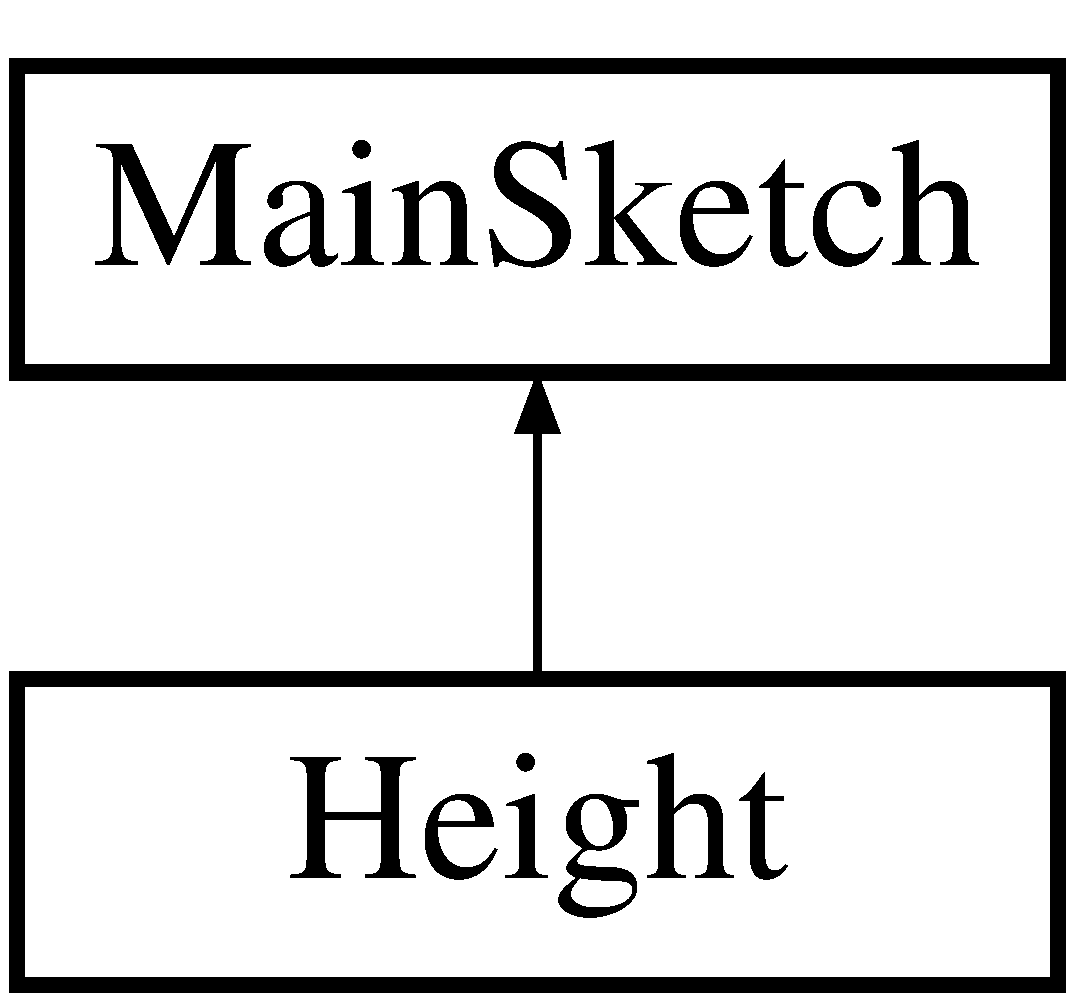
\includegraphics[height=2.000000cm]{classHeight}
\end{center}
\end{figure}
\subsection*{Public Member Functions}
\begin{DoxyCompactItemize}
\item 
void \hyperlink{classHeight_a62695cd45bcf1f441a73959774ef1151}{setup} ()
\begin{DoxyCompactList}\small\item\em pure virtual function for setup. Sublcasses must define \end{DoxyCompactList}\item 
void \hyperlink{classHeight_aa39bf5774d0ddf8e853d600dc70fd443}{loop} ()
\begin{DoxyCompactList}\small\item\em pure virtual function for loop. Sublcasses must define \end{DoxyCompactList}\end{DoxyCompactItemize}
\subsection*{Private Attributes}
\begin{DoxyCompactItemize}
\item 
\hyperlink{classFireFinder}{Fire\-Finder} \hyperlink{classHeight_a9cb83b4ed7622c3961552cf8f383d1b0}{ff}
\end{DoxyCompactItemize}


\subsection{Detailed Description}


Definition at line 7 of file Height.\-hpp.



\subsection{Member Function Documentation}
\hypertarget{classHeight_aa39bf5774d0ddf8e853d600dc70fd443}{\index{Height@{Height}!loop@{loop}}
\index{loop@{loop}!Height@{Height}}
\subsubsection[{loop}]{\setlength{\rightskip}{0pt plus 5cm}void Height\-::loop (
\begin{DoxyParamCaption}
{}
\end{DoxyParamCaption}
)\hspace{0.3cm}{\ttfamily [virtual]}}}\label{classHeight_aa39bf5774d0ddf8e853d600dc70fd443}


pure virtual function for loop. Sublcasses must define 



Implements \hyperlink{classMainSketch_acd69845de8c794dce73d309f142a6795}{Main\-Sketch}.



Definition at line 13 of file Height.\-cpp.

\hypertarget{classHeight_a62695cd45bcf1f441a73959774ef1151}{\index{Height@{Height}!setup@{setup}}
\index{setup@{setup}!Height@{Height}}
\subsubsection[{setup}]{\setlength{\rightskip}{0pt plus 5cm}void Height\-::setup (
\begin{DoxyParamCaption}
{}
\end{DoxyParamCaption}
)\hspace{0.3cm}{\ttfamily [virtual]}}}\label{classHeight_a62695cd45bcf1f441a73959774ef1151}


pure virtual function for setup. Sublcasses must define 



Implements \hyperlink{classMainSketch_a0708e1eb0ced1063f600f4111df90bf2}{Main\-Sketch}.



Definition at line 7 of file Height.\-cpp.



\subsection{Member Data Documentation}
\hypertarget{classHeight_a9cb83b4ed7622c3961552cf8f383d1b0}{\index{Height@{Height}!ff@{ff}}
\index{ff@{ff}!Height@{Height}}
\subsubsection[{ff}]{\setlength{\rightskip}{0pt plus 5cm}{\bf Fire\-Finder} Height\-::ff\hspace{0.3cm}{\ttfamily [private]}}}\label{classHeight_a9cb83b4ed7622c3961552cf8f383d1b0}


Definition at line 13 of file Height.\-hpp.



The documentation for this class was generated from the following files\-:\begin{DoxyCompactItemize}
\item 
src/test/\hyperlink{Height_8hpp}{Height.\-hpp}\item 
src/test/\hyperlink{Height_8cpp}{Height.\-cpp}\end{DoxyCompactItemize}

\hypertarget{classLidar}{\section{Lidar Class Reference}
\label{classLidar}\index{Lidar@{Lidar}}
}


{\ttfamily \#include $<$Lidar.\-hpp$>$}

\subsection*{Public Member Functions}
\begin{DoxyCompactItemize}
\item 
void \hyperlink{classLidar_abbb8e57bb39cb156cd03b9274843b32d}{setup} ()
\item 
bool \hyperlink{classLidar_a424a60f6278617333201c5fca115c288}{read} ()
\item 
void \hyperlink{classLidar_a64a54013a7ef0612c3c0f9f89dc93024}{process\-End\-Of\-Packet} ()
\item 
bool \hyperlink{classLidar_aefa743ccb6305927a312f9579e003f82}{is\-Data\-Index} (int index)
\end{DoxyCompactItemize}
\subsection*{Public Attributes}
\begin{DoxyCompactItemize}
\item 
int \hyperlink{classLidar_a5f97323ace606c1b4d2f817ebb8ebf7d}{distances} \mbox{[}360\mbox{]}
\item 
int \hyperlink{classLidar_a8eea2300d585c1b514ac6211a7326aca}{misses} = 0
\item 
int \hyperlink{classLidar_a43a0f4c1f8d6b0c9f1b21be32c99890d}{invalids}
\end{DoxyCompactItemize}
\subsection*{Private Attributes}
\begin{DoxyCompactItemize}
\item 
char \hyperlink{classLidar_a59f93afd1061d31642d1e7755838f2d1}{packet} \mbox{[}22\mbox{]}
\item 
bool \hyperlink{classLidar_a69b0909cc44f4e4e155d0ae2aa4ef3b4}{start\-Reading}
\item 
int \hyperlink{classLidar_a5e06436eae4b2d150501df175ec04758}{packet\-Index}
\item 
int \hyperlink{classLidar_a5d198ec3f5d3de7829dda616ea13d016}{distance\-Index}
\item 
int \hyperlink{classLidar_abcca8f7f6c4cff325e6b225ddbe14796}{packet\-Number}
\end{DoxyCompactItemize}


\subsection{Detailed Description}


Definition at line 3 of file Lidar.\-hpp.



\subsection{Member Function Documentation}
\hypertarget{classLidar_aefa743ccb6305927a312f9579e003f82}{\index{Lidar@{Lidar}!is\-Data\-Index@{is\-Data\-Index}}
\index{is\-Data\-Index@{is\-Data\-Index}!Lidar@{Lidar}}
\subsubsection[{is\-Data\-Index}]{\setlength{\rightskip}{0pt plus 5cm}bool Lidar\-::is\-Data\-Index (
\begin{DoxyParamCaption}
\item[{int}]{index}
\end{DoxyParamCaption}
)}}\label{classLidar_aefa743ccb6305927a312f9579e003f82}


Definition at line 89 of file Lidar.\-cpp.

\hypertarget{classLidar_a64a54013a7ef0612c3c0f9f89dc93024}{\index{Lidar@{Lidar}!process\-End\-Of\-Packet@{process\-End\-Of\-Packet}}
\index{process\-End\-Of\-Packet@{process\-End\-Of\-Packet}!Lidar@{Lidar}}
\subsubsection[{process\-End\-Of\-Packet}]{\setlength{\rightskip}{0pt plus 5cm}void Lidar\-::process\-End\-Of\-Packet (
\begin{DoxyParamCaption}
{}
\end{DoxyParamCaption}
)}}\label{classLidar_a64a54013a7ef0612c3c0f9f89dc93024}


Definition at line 51 of file Lidar.\-cpp.

\hypertarget{classLidar_a424a60f6278617333201c5fca115c288}{\index{Lidar@{Lidar}!read@{read}}
\index{read@{read}!Lidar@{Lidar}}
\subsubsection[{read}]{\setlength{\rightskip}{0pt plus 5cm}bool Lidar\-::read (
\begin{DoxyParamCaption}
{}
\end{DoxyParamCaption}
)}}\label{classLidar_a424a60f6278617333201c5fca115c288}


Definition at line 16 of file Lidar.\-cpp.

\hypertarget{classLidar_abbb8e57bb39cb156cd03b9274843b32d}{\index{Lidar@{Lidar}!setup@{setup}}
\index{setup@{setup}!Lidar@{Lidar}}
\subsubsection[{setup}]{\setlength{\rightskip}{0pt plus 5cm}void Lidar\-::setup (
\begin{DoxyParamCaption}
{}
\end{DoxyParamCaption}
)}}\label{classLidar_abbb8e57bb39cb156cd03b9274843b32d}


Definition at line 4 of file Lidar.\-cpp.



\subsection{Member Data Documentation}
\hypertarget{classLidar_a5d198ec3f5d3de7829dda616ea13d016}{\index{Lidar@{Lidar}!distance\-Index@{distance\-Index}}
\index{distance\-Index@{distance\-Index}!Lidar@{Lidar}}
\subsubsection[{distance\-Index}]{\setlength{\rightskip}{0pt plus 5cm}int Lidar\-::distance\-Index\hspace{0.3cm}{\ttfamily [private]}}}\label{classLidar_a5d198ec3f5d3de7829dda616ea13d016}


Definition at line 27 of file Lidar.\-hpp.

\hypertarget{classLidar_a5f97323ace606c1b4d2f817ebb8ebf7d}{\index{Lidar@{Lidar}!distances@{distances}}
\index{distances@{distances}!Lidar@{Lidar}}
\subsubsection[{distances}]{\setlength{\rightskip}{0pt plus 5cm}int Lidar\-::distances\mbox{[}360\mbox{]}}}\label{classLidar_a5f97323ace606c1b4d2f817ebb8ebf7d}


Definition at line 6 of file Lidar.\-hpp.

\hypertarget{classLidar_a43a0f4c1f8d6b0c9f1b21be32c99890d}{\index{Lidar@{Lidar}!invalids@{invalids}}
\index{invalids@{invalids}!Lidar@{Lidar}}
\subsubsection[{invalids}]{\setlength{\rightskip}{0pt plus 5cm}int Lidar\-::invalids}}\label{classLidar_a43a0f4c1f8d6b0c9f1b21be32c99890d}
the number of invalids during each sweep 

Definition at line 12 of file Lidar.\-hpp.

\hypertarget{classLidar_a8eea2300d585c1b514ac6211a7326aca}{\index{Lidar@{Lidar}!misses@{misses}}
\index{misses@{misses}!Lidar@{Lidar}}
\subsubsection[{misses}]{\setlength{\rightskip}{0pt plus 5cm}int Lidar\-::misses = 0}}\label{classLidar_a8eea2300d585c1b514ac6211a7326aca}
the number of missed packets during each sweep 

Definition at line 9 of file Lidar.\-hpp.

\hypertarget{classLidar_a59f93afd1061d31642d1e7755838f2d1}{\index{Lidar@{Lidar}!packet@{packet}}
\index{packet@{packet}!Lidar@{Lidar}}
\subsubsection[{packet}]{\setlength{\rightskip}{0pt plus 5cm}char Lidar\-::packet\mbox{[}22\mbox{]}\hspace{0.3cm}{\ttfamily [private]}}}\label{classLidar_a59f93afd1061d31642d1e7755838f2d1}


Definition at line 23 of file Lidar.\-hpp.

\hypertarget{classLidar_a5e06436eae4b2d150501df175ec04758}{\index{Lidar@{Lidar}!packet\-Index@{packet\-Index}}
\index{packet\-Index@{packet\-Index}!Lidar@{Lidar}}
\subsubsection[{packet\-Index}]{\setlength{\rightskip}{0pt plus 5cm}int Lidar\-::packet\-Index\hspace{0.3cm}{\ttfamily [private]}}}\label{classLidar_a5e06436eae4b2d150501df175ec04758}


Definition at line 27 of file Lidar.\-hpp.

\hypertarget{classLidar_abcca8f7f6c4cff325e6b225ddbe14796}{\index{Lidar@{Lidar}!packet\-Number@{packet\-Number}}
\index{packet\-Number@{packet\-Number}!Lidar@{Lidar}}
\subsubsection[{packet\-Number}]{\setlength{\rightskip}{0pt plus 5cm}int Lidar\-::packet\-Number\hspace{0.3cm}{\ttfamily [private]}}}\label{classLidar_abcca8f7f6c4cff325e6b225ddbe14796}


Definition at line 30 of file Lidar.\-hpp.

\hypertarget{classLidar_a69b0909cc44f4e4e155d0ae2aa4ef3b4}{\index{Lidar@{Lidar}!start\-Reading@{start\-Reading}}
\index{start\-Reading@{start\-Reading}!Lidar@{Lidar}}
\subsubsection[{start\-Reading}]{\setlength{\rightskip}{0pt plus 5cm}bool Lidar\-::start\-Reading\hspace{0.3cm}{\ttfamily [private]}}}\label{classLidar_a69b0909cc44f4e4e155d0ae2aa4ef3b4}


Definition at line 25 of file Lidar.\-hpp.



The documentation for this class was generated from the following files\-:\begin{DoxyCompactItemize}
\item 
src/shared/\hyperlink{Lidar_8hpp}{Lidar.\-hpp}\item 
src/shared/\hyperlink{Lidar_8cpp}{Lidar.\-cpp}\end{DoxyCompactItemize}

\hypertarget{classLidarBenchmark}{\section{Lidar\-Benchmark Class Reference}
\label{classLidarBenchmark}\index{Lidar\-Benchmark@{Lidar\-Benchmark}}
}


{\ttfamily \#include $<$Lidar\-Benchmark.\-hpp$>$}

Inheritance diagram for Lidar\-Benchmark\-:\begin{figure}[H]
\begin{center}
\leavevmode
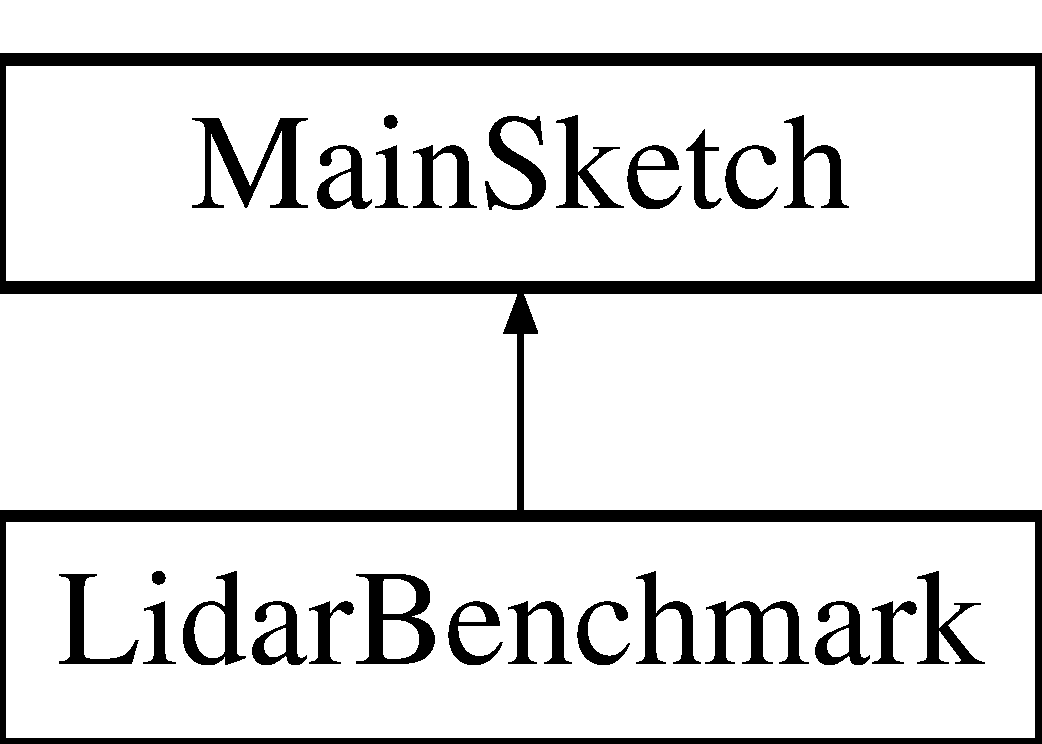
\includegraphics[height=2.000000cm]{classLidarBenchmark}
\end{center}
\end{figure}
\subsection*{Public Member Functions}
\begin{DoxyCompactItemize}
\item 
void \hyperlink{classLidarBenchmark_a8e8ccd212f927ba3ca36bc1e3daba4ec}{setup} ()
\item 
void \hyperlink{classLidarBenchmark_a0bfe575d370277a4e594bcae1b6f9a1a}{loop} ()
\end{DoxyCompactItemize}
\subsection*{Private Attributes}
\begin{DoxyCompactItemize}
\item 
\hyperlink{classLidar}{Lidar} \hyperlink{classLidarBenchmark_a559db88ad7e51c4c254ce241c0361ab6}{lidar}
\item 
long \hyperlink{classLidarBenchmark_a5527736a3831d0a04d8158748e8f2b48}{t0}
\end{DoxyCompactItemize}


\subsection{Detailed Description}


Definition at line 7 of file Lidar\-Benchmark.\-hpp.



\subsection{Member Function Documentation}
\hypertarget{classLidarBenchmark_a0bfe575d370277a4e594bcae1b6f9a1a}{\index{Lidar\-Benchmark@{Lidar\-Benchmark}!loop@{loop}}
\index{loop@{loop}!LidarBenchmark@{Lidar\-Benchmark}}
\subsubsection[{loop}]{\setlength{\rightskip}{0pt plus 5cm}void Lidar\-Benchmark\-::loop (
\begin{DoxyParamCaption}
{}
\end{DoxyParamCaption}
)\hspace{0.3cm}{\ttfamily [virtual]}}}\label{classLidarBenchmark_a0bfe575d370277a4e594bcae1b6f9a1a}


Implements \hyperlink{classMainSketch_acd69845de8c794dce73d309f142a6795}{Main\-Sketch}.



Definition at line 12 of file Lidar\-Benchmark.\-cpp.

\hypertarget{classLidarBenchmark_a8e8ccd212f927ba3ca36bc1e3daba4ec}{\index{Lidar\-Benchmark@{Lidar\-Benchmark}!setup@{setup}}
\index{setup@{setup}!LidarBenchmark@{Lidar\-Benchmark}}
\subsubsection[{setup}]{\setlength{\rightskip}{0pt plus 5cm}void Lidar\-Benchmark\-::setup (
\begin{DoxyParamCaption}
{}
\end{DoxyParamCaption}
)\hspace{0.3cm}{\ttfamily [virtual]}}}\label{classLidarBenchmark_a8e8ccd212f927ba3ca36bc1e3daba4ec}


Implements \hyperlink{classMainSketch_a0708e1eb0ced1063f600f4111df90bf2}{Main\-Sketch}.



Definition at line 6 of file Lidar\-Benchmark.\-cpp.



\subsection{Member Data Documentation}
\hypertarget{classLidarBenchmark_a559db88ad7e51c4c254ce241c0361ab6}{\index{Lidar\-Benchmark@{Lidar\-Benchmark}!lidar@{lidar}}
\index{lidar@{lidar}!LidarBenchmark@{Lidar\-Benchmark}}
\subsubsection[{lidar}]{\setlength{\rightskip}{0pt plus 5cm}{\bf Lidar} Lidar\-Benchmark\-::lidar\hspace{0.3cm}{\ttfamily [private]}}}\label{classLidarBenchmark_a559db88ad7e51c4c254ce241c0361ab6}


Definition at line 13 of file Lidar\-Benchmark.\-hpp.

\hypertarget{classLidarBenchmark_a5527736a3831d0a04d8158748e8f2b48}{\index{Lidar\-Benchmark@{Lidar\-Benchmark}!t0@{t0}}
\index{t0@{t0}!LidarBenchmark@{Lidar\-Benchmark}}
\subsubsection[{t0}]{\setlength{\rightskip}{0pt plus 5cm}long Lidar\-Benchmark\-::t0\hspace{0.3cm}{\ttfamily [private]}}}\label{classLidarBenchmark_a5527736a3831d0a04d8158748e8f2b48}


Definition at line 14 of file Lidar\-Benchmark.\-hpp.



The documentation for this class was generated from the following files\-:\begin{DoxyCompactItemize}
\item 
src/test/\hyperlink{LidarBenchmark_8hpp}{Lidar\-Benchmark.\-hpp}\item 
src/test/\hyperlink{LidarBenchmark_8cpp}{Lidar\-Benchmark.\-cpp}\end{DoxyCompactItemize}

\hypertarget{classLidarDump}{\section{Lidar\-Dump Class Reference}
\label{classLidarDump}\index{Lidar\-Dump@{Lidar\-Dump}}
}


{\ttfamily \#include $<$Lidar\-Dump.\-hpp$>$}

\subsection*{Public Member Functions}
\begin{DoxyCompactItemize}
\item 
void \hyperlink{classLidarDump_ad0368709dae4efa58d381fa252245360}{setup} ()
\item 
void \hyperlink{classLidarDump_a869f5113612b4b1a7920f736e1587861}{loop} ()
\end{DoxyCompactItemize}
\subsection*{Private Attributes}
\begin{DoxyCompactItemize}
\item 
\hyperlink{classRobot}{Robot} $\ast$ \hyperlink{classLidarDump_a855703e06ed680346b0f6accecf17b11}{charizard}
\item 
bool \hyperlink{classLidarDump_a2b76c3131d789b4eb45f92c6b9847f82}{reading}
\item 
int \hyperlink{classLidarDump_a0d68951dd2bd7da58bde795c76979e0e}{count}
\end{DoxyCompactItemize}


\subsection{Detailed Description}


Definition at line 3 of file Lidar\-Dump.\-hpp.



\subsection{Member Function Documentation}
\hypertarget{classLidarDump_a869f5113612b4b1a7920f736e1587861}{\index{Lidar\-Dump@{Lidar\-Dump}!loop@{loop}}
\index{loop@{loop}!LidarDump@{Lidar\-Dump}}
\subsubsection[{loop}]{\setlength{\rightskip}{0pt plus 5cm}void Lidar\-Dump\-::loop (
\begin{DoxyParamCaption}
{}
\end{DoxyParamCaption}
)}}\label{classLidarDump_a869f5113612b4b1a7920f736e1587861}


Definition at line 10 of file Lidar\-Dump.\-cpp.

\hypertarget{classLidarDump_ad0368709dae4efa58d381fa252245360}{\index{Lidar\-Dump@{Lidar\-Dump}!setup@{setup}}
\index{setup@{setup}!LidarDump@{Lidar\-Dump}}
\subsubsection[{setup}]{\setlength{\rightskip}{0pt plus 5cm}void Lidar\-Dump\-::setup (
\begin{DoxyParamCaption}
{}
\end{DoxyParamCaption}
)}}\label{classLidarDump_ad0368709dae4efa58d381fa252245360}


Definition at line 3 of file Lidar\-Dump.\-cpp.



\subsection{Member Data Documentation}
\hypertarget{classLidarDump_a855703e06ed680346b0f6accecf17b11}{\index{Lidar\-Dump@{Lidar\-Dump}!charizard@{charizard}}
\index{charizard@{charizard}!LidarDump@{Lidar\-Dump}}
\subsubsection[{charizard}]{\setlength{\rightskip}{0pt plus 5cm}{\bf Robot}$\ast$ Lidar\-Dump\-::charizard\hspace{0.3cm}{\ttfamily [private]}}}\label{classLidarDump_a855703e06ed680346b0f6accecf17b11}


Definition at line 8 of file Lidar\-Dump.\-hpp.

\hypertarget{classLidarDump_a0d68951dd2bd7da58bde795c76979e0e}{\index{Lidar\-Dump@{Lidar\-Dump}!count@{count}}
\index{count@{count}!LidarDump@{Lidar\-Dump}}
\subsubsection[{count}]{\setlength{\rightskip}{0pt plus 5cm}int Lidar\-Dump\-::count\hspace{0.3cm}{\ttfamily [private]}}}\label{classLidarDump_a0d68951dd2bd7da58bde795c76979e0e}


Definition at line 10 of file Lidar\-Dump.\-hpp.

\hypertarget{classLidarDump_a2b76c3131d789b4eb45f92c6b9847f82}{\index{Lidar\-Dump@{Lidar\-Dump}!reading@{reading}}
\index{reading@{reading}!LidarDump@{Lidar\-Dump}}
\subsubsection[{reading}]{\setlength{\rightskip}{0pt plus 5cm}bool Lidar\-Dump\-::reading\hspace{0.3cm}{\ttfamily [private]}}}\label{classLidarDump_a2b76c3131d789b4eb45f92c6b9847f82}


Definition at line 9 of file Lidar\-Dump.\-hpp.



The documentation for this class was generated from the following files\-:\begin{DoxyCompactItemize}
\item 
src/test/\hyperlink{LidarDump_8hpp}{Lidar\-Dump.\-hpp}\item 
src/test/\hyperlink{LidarDump_8cpp}{Lidar\-Dump.\-cpp}\end{DoxyCompactItemize}

\hypertarget{classMain}{\section{Main Class Reference}
\label{classMain}\index{Main@{Main}}
}


\hyperlink{classMain}{Main} is the highest level state machine for the robot.  




{\ttfamily \#include $<$Main.\-hpp$>$}

\subsection*{Public Member Functions}
\begin{DoxyCompactItemize}
\item 
void \hyperlink{classMain_ab93af44e220d33016f01ed1b70612899}{setup} ()
\begin{DoxyCompactList}\small\item\em setup method calls setup for robot \end{DoxyCompactList}\item 
void \hyperlink{classMain_ac061692135a219ec5b7a8211c4e26ed6}{loop} ()
\begin{DoxyCompactList}\small\item\em main state machine controls overall program flow \end{DoxyCompactList}\item 
void \hyperlink{classMain_a2c24ed69c03010e24c109b7b4d59eca1}{change\-State} (\hyperlink{classMain_a551231243a758b95cf29d8ed2b7508da}{State} \hyperlink{classMain_a8b4ada43c3c3720b177018191ac6ee90}{state})
\begin{DoxyCompactList}\small\item\em change state and print state \end{DoxyCompactList}\end{DoxyCompactItemize}
\subsection*{Private Types}
\begin{DoxyCompactItemize}
\item 
enum \hyperlink{classMain_a551231243a758b95cf29d8ed2b7508da}{State} \{ \\*
\hyperlink{classMain_a551231243a758b95cf29d8ed2b7508daa9229c9e5dce20fda7fd5bbd54799fb32}{S\-E\-A\-R\-C\-H\-\_\-\-F\-O\-R\-\_\-\-C\-A\-N\-D\-L\-E}, 
\hyperlink{classMain_a551231243a758b95cf29d8ed2b7508daab2b9975fcdb8d0d79230156c24adf5b4}{F\-I\-N\-D\-\_\-\-C\-A\-N\-D\-L\-E\-\_\-\-H\-E\-I\-G\-H\-T}, 
\hyperlink{classMain_a551231243a758b95cf29d8ed2b7508daaf335b92cf0219a9b661613556bbe96b6}{E\-X\-T\-I\-N\-G\-U\-I\-S\-H\-\_\-\-C\-A\-N\-D\-L\-E}, 
\hyperlink{classMain_a551231243a758b95cf29d8ed2b7508daa3ff87a64146af251296a5ce0a05e923d}{R\-E\-T\-U\-R\-N\-\_\-\-T\-O\-\_\-\-O\-R\-I\-G\-I\-N}, 
\\*
\hyperlink{classMain_a551231243a758b95cf29d8ed2b7508daa6c2f5ff7b13123b1b782ac3664f20087}{E\-N\-D}
 \}
\begin{DoxyCompactList}\small\item\em The main states of the robot. \end{DoxyCompactList}\end{DoxyCompactItemize}
\subsection*{Private Attributes}
\begin{DoxyCompactItemize}
\item 
char $\ast$ \hyperlink{classMain_a10090d1fa7fa606c1bf7c5bdf23d7eda}{state\-Names} \mbox{[}5\mbox{]}
\begin{DoxyCompactList}\small\item\em English state names allows us to easily print what state the robot is in. \end{DoxyCompactList}\item 
\hyperlink{classMain_a551231243a758b95cf29d8ed2b7508da}{State} \hyperlink{classMain_a8b4ada43c3c3720b177018191ac6ee90}{state} = \hyperlink{classMain_a551231243a758b95cf29d8ed2b7508daa9229c9e5dce20fda7fd5bbd54799fb32}{S\-E\-A\-R\-C\-H\-\_\-\-F\-O\-R\-\_\-\-C\-A\-N\-D\-L\-E}
\begin{DoxyCompactList}\small\item\em variable for the current state of the robot. \end{DoxyCompactList}\item 
\hyperlink{classRobot}{Robot} $\ast$ \hyperlink{classMain_a6b8534d72e39e2b43c3d46f2ca6e49f4}{charizard}
\begin{DoxyCompactList}\small\item\em convenient pointer to the singleton robot instance \end{DoxyCompactList}\end{DoxyCompactItemize}


\subsection{Detailed Description}
\hyperlink{classMain}{Main} is the highest level state machine for the robot. 

Definition at line 6 of file Main.\-hpp.



\subsection{Member Enumeration Documentation}
\hypertarget{classMain_a551231243a758b95cf29d8ed2b7508da}{\index{Main@{Main}!State@{State}}
\index{State@{State}!Main@{Main}}
\subsubsection[{State}]{\setlength{\rightskip}{0pt plus 5cm}enum {\bf Main\-::\-State}\hspace{0.3cm}{\ttfamily [private]}}}\label{classMain_a551231243a758b95cf29d8ed2b7508da}


The main states of the robot. 

\begin{Desc}
\item[Enumerator]\par
\begin{description}
\index{S\-E\-A\-R\-C\-H\-\_\-\-F\-O\-R\-\_\-\-C\-A\-N\-D\-L\-E@{S\-E\-A\-R\-C\-H\-\_\-\-F\-O\-R\-\_\-\-C\-A\-N\-D\-L\-E}!Main@{Main}}\index{Main@{Main}!S\-E\-A\-R\-C\-H\-\_\-\-F\-O\-R\-\_\-\-C\-A\-N\-D\-L\-E@{S\-E\-A\-R\-C\-H\-\_\-\-F\-O\-R\-\_\-\-C\-A\-N\-D\-L\-E}}\item[{\em 
\hypertarget{classMain_a551231243a758b95cf29d8ed2b7508daa9229c9e5dce20fda7fd5bbd54799fb32}{S\-E\-A\-R\-C\-H\-\_\-\-F\-O\-R\-\_\-\-C\-A\-N\-D\-L\-E}\label{classMain_a551231243a758b95cf29d8ed2b7508daa9229c9e5dce20fda7fd5bbd54799fb32}
}]\index{F\-I\-N\-D\-\_\-\-C\-A\-N\-D\-L\-E\-\_\-\-H\-E\-I\-G\-H\-T@{F\-I\-N\-D\-\_\-\-C\-A\-N\-D\-L\-E\-\_\-\-H\-E\-I\-G\-H\-T}!Main@{Main}}\index{Main@{Main}!F\-I\-N\-D\-\_\-\-C\-A\-N\-D\-L\-E\-\_\-\-H\-E\-I\-G\-H\-T@{F\-I\-N\-D\-\_\-\-C\-A\-N\-D\-L\-E\-\_\-\-H\-E\-I\-G\-H\-T}}\item[{\em 
\hypertarget{classMain_a551231243a758b95cf29d8ed2b7508daab2b9975fcdb8d0d79230156c24adf5b4}{F\-I\-N\-D\-\_\-\-C\-A\-N\-D\-L\-E\-\_\-\-H\-E\-I\-G\-H\-T}\label{classMain_a551231243a758b95cf29d8ed2b7508daab2b9975fcdb8d0d79230156c24adf5b4}
}]\index{E\-X\-T\-I\-N\-G\-U\-I\-S\-H\-\_\-\-C\-A\-N\-D\-L\-E@{E\-X\-T\-I\-N\-G\-U\-I\-S\-H\-\_\-\-C\-A\-N\-D\-L\-E}!Main@{Main}}\index{Main@{Main}!E\-X\-T\-I\-N\-G\-U\-I\-S\-H\-\_\-\-C\-A\-N\-D\-L\-E@{E\-X\-T\-I\-N\-G\-U\-I\-S\-H\-\_\-\-C\-A\-N\-D\-L\-E}}\item[{\em 
\hypertarget{classMain_a551231243a758b95cf29d8ed2b7508daaf335b92cf0219a9b661613556bbe96b6}{E\-X\-T\-I\-N\-G\-U\-I\-S\-H\-\_\-\-C\-A\-N\-D\-L\-E}\label{classMain_a551231243a758b95cf29d8ed2b7508daaf335b92cf0219a9b661613556bbe96b6}
}]\index{R\-E\-T\-U\-R\-N\-\_\-\-T\-O\-\_\-\-O\-R\-I\-G\-I\-N@{R\-E\-T\-U\-R\-N\-\_\-\-T\-O\-\_\-\-O\-R\-I\-G\-I\-N}!Main@{Main}}\index{Main@{Main}!R\-E\-T\-U\-R\-N\-\_\-\-T\-O\-\_\-\-O\-R\-I\-G\-I\-N@{R\-E\-T\-U\-R\-N\-\_\-\-T\-O\-\_\-\-O\-R\-I\-G\-I\-N}}\item[{\em 
\hypertarget{classMain_a551231243a758b95cf29d8ed2b7508daa3ff87a64146af251296a5ce0a05e923d}{R\-E\-T\-U\-R\-N\-\_\-\-T\-O\-\_\-\-O\-R\-I\-G\-I\-N}\label{classMain_a551231243a758b95cf29d8ed2b7508daa3ff87a64146af251296a5ce0a05e923d}
}]\index{E\-N\-D@{E\-N\-D}!Main@{Main}}\index{Main@{Main}!E\-N\-D@{E\-N\-D}}\item[{\em 
\hypertarget{classMain_a551231243a758b95cf29d8ed2b7508daa6c2f5ff7b13123b1b782ac3664f20087}{E\-N\-D}\label{classMain_a551231243a758b95cf29d8ed2b7508daa6c2f5ff7b13123b1b782ac3664f20087}
}]\end{description}
\end{Desc}


Definition at line 9 of file Main.\-hpp.



\subsection{Member Function Documentation}
\hypertarget{classMain_a2c24ed69c03010e24c109b7b4d59eca1}{\index{Main@{Main}!change\-State@{change\-State}}
\index{change\-State@{change\-State}!Main@{Main}}
\subsubsection[{change\-State}]{\setlength{\rightskip}{0pt plus 5cm}void Main\-::change\-State (
\begin{DoxyParamCaption}
\item[{{\bf State}}]{state}
\end{DoxyParamCaption}
)}}\label{classMain_a2c24ed69c03010e24c109b7b4d59eca1}


change state and print state 



Definition at line 12 of file Main.\-cpp.

\hypertarget{classMain_ac061692135a219ec5b7a8211c4e26ed6}{\index{Main@{Main}!loop@{loop}}
\index{loop@{loop}!Main@{Main}}
\subsubsection[{loop}]{\setlength{\rightskip}{0pt plus 5cm}void Main\-::loop (
\begin{DoxyParamCaption}
{}
\end{DoxyParamCaption}
)}}\label{classMain_ac061692135a219ec5b7a8211c4e26ed6}


main state machine controls overall program flow 



Definition at line 17 of file Main.\-cpp.

\hypertarget{classMain_ab93af44e220d33016f01ed1b70612899}{\index{Main@{Main}!setup@{setup}}
\index{setup@{setup}!Main@{Main}}
\subsubsection[{setup}]{\setlength{\rightskip}{0pt plus 5cm}void Main\-::setup (
\begin{DoxyParamCaption}
{}
\end{DoxyParamCaption}
)}}\label{classMain_ab93af44e220d33016f01ed1b70612899}


setup method calls setup for robot 



Definition at line 6 of file Main.\-cpp.



\subsection{Member Data Documentation}
\hypertarget{classMain_a6b8534d72e39e2b43c3d46f2ca6e49f4}{\index{Main@{Main}!charizard@{charizard}}
\index{charizard@{charizard}!Main@{Main}}
\subsubsection[{charizard}]{\setlength{\rightskip}{0pt plus 5cm}{\bf Robot}$\ast$ Main\-::charizard\hspace{0.3cm}{\ttfamily [private]}}}\label{classMain_a6b8534d72e39e2b43c3d46f2ca6e49f4}


convenient pointer to the singleton robot instance 



Definition at line 42 of file Main.\-hpp.

\hypertarget{classMain_a8b4ada43c3c3720b177018191ac6ee90}{\index{Main@{Main}!state@{state}}
\index{state@{state}!Main@{Main}}
\subsubsection[{state}]{\setlength{\rightskip}{0pt plus 5cm}{\bf State} Main\-::state = {\bf S\-E\-A\-R\-C\-H\-\_\-\-F\-O\-R\-\_\-\-C\-A\-N\-D\-L\-E}\hspace{0.3cm}{\ttfamily [private]}}}\label{classMain_a8b4ada43c3c3720b177018191ac6ee90}


variable for the current state of the robot. 



Definition at line 39 of file Main.\-hpp.

\hypertarget{classMain_a10090d1fa7fa606c1bf7c5bdf23d7eda}{\index{Main@{Main}!state\-Names@{state\-Names}}
\index{state\-Names@{state\-Names}!Main@{Main}}
\subsubsection[{state\-Names}]{\setlength{\rightskip}{0pt plus 5cm}char$\ast$ Main\-::state\-Names\mbox{[}5\mbox{]}\hspace{0.3cm}{\ttfamily [private]}}}\label{classMain_a10090d1fa7fa606c1bf7c5bdf23d7eda}
{\bfseries Initial value\-:}
\begin{DoxyCode}
= \{
      \textcolor{stringliteral}{"SEARCH\_4\_CANDLE "},
      \textcolor{stringliteral}{"CANDLE\_HEIGHT   "},
      \textcolor{stringliteral}{"EXNTIGISH\_CANDLE"},
      \textcolor{stringliteral}{"RETRN\_TO\_ORGIN  "},
      \textcolor{stringliteral}{"END             "}\}
\end{DoxyCode}


English state names allows us to easily print what state the robot is in. 



Definition at line 31 of file Main.\-hpp.



The documentation for this class was generated from the following files\-:\begin{DoxyCompactItemize}
\item 
src/\hyperlink{Main_8hpp}{Main.\-hpp}\item 
src/\hyperlink{Main_8cpp}{Main.\-cpp}\end{DoxyCompactItemize}

\hypertarget{classMainSketch}{\section{Main\-Sketch Class Reference}
\label{classMainSketch}\index{Main\-Sketch@{Main\-Sketch}}
}


This class is used by charizard. \hyperlink{classMain}{Main} and other test sketches should extend this class and implement setup and loop.  




{\ttfamily \#include $<$Main\-Sketch.\-hpp$>$}

\subsection*{Public Member Functions}
\begin{DoxyCompactItemize}
\item 
virtual void \hyperlink{classMainSketch_a0708e1eb0ced1063f600f4111df90bf2}{setup} ()=0
\begin{DoxyCompactList}\small\item\em pure virtual function for setup. Sublcasses must define \end{DoxyCompactList}\item 
virtual void \hyperlink{classMainSketch_acd69845de8c794dce73d309f142a6795}{loop} ()=0
\begin{DoxyCompactList}\small\item\em pure virtual function for loop. Sublcasses must define \end{DoxyCompactList}\end{DoxyCompactItemize}


\subsection{Detailed Description}
This class is used by charizard. \hyperlink{classMain}{Main} and other test sketches should extend this class and implement setup and loop. 

Definition at line 9 of file Main\-Sketch.\-hpp.



\subsection{Member Function Documentation}
\hypertarget{classMainSketch_acd69845de8c794dce73d309f142a6795}{\index{Main\-Sketch@{Main\-Sketch}!loop@{loop}}
\index{loop@{loop}!MainSketch@{Main\-Sketch}}
\subsubsection[{loop}]{\setlength{\rightskip}{0pt plus 5cm}virtual void Main\-Sketch\-::loop (
\begin{DoxyParamCaption}
{}
\end{DoxyParamCaption}
)\hspace{0.3cm}{\ttfamily [pure virtual]}}}\label{classMainSketch_acd69845de8c794dce73d309f142a6795}


pure virtual function for loop. Sublcasses must define 

\hypertarget{classMainSketch_a0708e1eb0ced1063f600f4111df90bf2}{\index{Main\-Sketch@{Main\-Sketch}!setup@{setup}}
\index{setup@{setup}!MainSketch@{Main\-Sketch}}
\subsubsection[{setup}]{\setlength{\rightskip}{0pt plus 5cm}virtual void Main\-Sketch\-::setup (
\begin{DoxyParamCaption}
{}
\end{DoxyParamCaption}
)\hspace{0.3cm}{\ttfamily [pure virtual]}}}\label{classMainSketch_a0708e1eb0ced1063f600f4111df90bf2}


pure virtual function for setup. Sublcasses must define 



The documentation for this class was generated from the following file\-:\begin{DoxyCompactItemize}
\item 
src/\hyperlink{MainSketch_8hpp}{Main\-Sketch.\-hpp}\end{DoxyCompactItemize}

\hypertarget{classNavigator}{\section{Navigator Class Reference}
\label{classNavigator}\index{Navigator@{Navigator}}
}


{\ttfamily \#include $<$Navigator.\-hpp$>$}

\subsection*{Public Member Functions}
\begin{DoxyCompactItemize}
\item 
\hyperlink{classNavigator_a59230ab4698882f754d5ce275a1a4030}{Navigator} ()
\item 
void \hyperlink{classNavigator_a14da808a74fdc15ae4e0781060884ef8}{set\-Goal} (\hyperlink{classPoint}{Point}$<$ float $>$ goal)
\begin{DoxyCompactList}\small\item\em set the goal to drive to This also resets the internal state \end{DoxyCompactList}\item 
bool \hyperlink{classNavigator_a8841b985afa17a86112b8522ee6913e6}{run} ()
\begin{DoxyCompactList}\small\item\em drive to the point \end{DoxyCompactList}\end{DoxyCompactItemize}
\subsection*{Private Types}
\begin{DoxyCompactItemize}
\item 
enum \hyperlink{classNavigator_aae36be38543e3fae30dc53208e2f9913}{State} \{ \hyperlink{classNavigator_aae36be38543e3fae30dc53208e2f9913a80d7d232a04edaac4c8055a05242790b}{T\-U\-R\-N\-I\-N\-G}, 
\hyperlink{classNavigator_aae36be38543e3fae30dc53208e2f9913a9f34e19722c2c3385c6fe61d8de249e7}{D\-R\-I\-V\-I\-N\-G}
 \}
\end{DoxyCompactItemize}
\subsection*{Private Attributes}
\begin{DoxyCompactItemize}
\item 
\hyperlink{classPID}{P\-I\-D} \hyperlink{classNavigator_ab6f4e8b5937d700d4514c438cb7b3927}{dist\-Pid}
\item 
float \hyperlink{classNavigator_a20335cc0cf85bdd18af14ee2dfbd1501}{angle}
\item 
float \hyperlink{classNavigator_accc10be1bc4dfe67ce799e69869f0caa}{distance}
\item 
enum \hyperlink{classNavigator_aae36be38543e3fae30dc53208e2f9913}{Navigator\-::\-State} \hyperlink{classNavigator_a15263fe64d0ea29a1bbfe9e5ef849c4c}{state}
\end{DoxyCompactItemize}


\subsection{Detailed Description}


Definition at line 5 of file Navigator.\-hpp.



\subsection{Member Enumeration Documentation}
\hypertarget{classNavigator_aae36be38543e3fae30dc53208e2f9913}{\index{Navigator@{Navigator}!State@{State}}
\index{State@{State}!Navigator@{Navigator}}
\subsubsection[{State}]{\setlength{\rightskip}{0pt plus 5cm}enum {\bf Navigator\-::\-State}\hspace{0.3cm}{\ttfamily [private]}}}\label{classNavigator_aae36be38543e3fae30dc53208e2f9913}
\begin{Desc}
\item[Enumerator]\par
\begin{description}
\index{T\-U\-R\-N\-I\-N\-G@{T\-U\-R\-N\-I\-N\-G}!Navigator@{Navigator}}\index{Navigator@{Navigator}!T\-U\-R\-N\-I\-N\-G@{T\-U\-R\-N\-I\-N\-G}}\item[{\em 
\hypertarget{classNavigator_aae36be38543e3fae30dc53208e2f9913a80d7d232a04edaac4c8055a05242790b}{T\-U\-R\-N\-I\-N\-G}\label{classNavigator_aae36be38543e3fae30dc53208e2f9913a80d7d232a04edaac4c8055a05242790b}
}]\index{D\-R\-I\-V\-I\-N\-G@{D\-R\-I\-V\-I\-N\-G}!Navigator@{Navigator}}\index{Navigator@{Navigator}!D\-R\-I\-V\-I\-N\-G@{D\-R\-I\-V\-I\-N\-G}}\item[{\em 
\hypertarget{classNavigator_aae36be38543e3fae30dc53208e2f9913a9f34e19722c2c3385c6fe61d8de249e7}{D\-R\-I\-V\-I\-N\-G}\label{classNavigator_aae36be38543e3fae30dc53208e2f9913a9f34e19722c2c3385c6fe61d8de249e7}
}]\end{description}
\end{Desc}


Definition at line 23 of file Navigator.\-hpp.



\subsection{Constructor \& Destructor Documentation}
\hypertarget{classNavigator_a59230ab4698882f754d5ce275a1a4030}{\index{Navigator@{Navigator}!Navigator@{Navigator}}
\index{Navigator@{Navigator}!Navigator@{Navigator}}
\subsubsection[{Navigator}]{\setlength{\rightskip}{0pt plus 5cm}Navigator\-::\-Navigator (
\begin{DoxyParamCaption}
{}
\end{DoxyParamCaption}
)}}\label{classNavigator_a59230ab4698882f754d5ce275a1a4030}


Definition at line 4 of file Navigator.\-cpp.



\subsection{Member Function Documentation}
\hypertarget{classNavigator_a8841b985afa17a86112b8522ee6913e6}{\index{Navigator@{Navigator}!run@{run}}
\index{run@{run}!Navigator@{Navigator}}
\subsubsection[{run}]{\setlength{\rightskip}{0pt plus 5cm}bool Navigator\-::run (
\begin{DoxyParamCaption}
{}
\end{DoxyParamCaption}
)}}\label{classNavigator_a8841b985afa17a86112b8522ee6913e6}


drive to the point 

\begin{DoxyReturn}{Returns}
true when the drive is complete 
\end{DoxyReturn}


Definition at line 16 of file Navigator.\-cpp.

\hypertarget{classNavigator_a14da808a74fdc15ae4e0781060884ef8}{\index{Navigator@{Navigator}!set\-Goal@{set\-Goal}}
\index{set\-Goal@{set\-Goal}!Navigator@{Navigator}}
\subsubsection[{set\-Goal}]{\setlength{\rightskip}{0pt plus 5cm}void Navigator\-::set\-Goal (
\begin{DoxyParamCaption}
\item[{{\bf Point}$<$ float $>$}]{goal}
\end{DoxyParamCaption}
)}}\label{classNavigator_a14da808a74fdc15ae4e0781060884ef8}


set the goal to drive to This also resets the internal state 


\begin{DoxyParams}{Parameters}
{\em goal} & the point to drive to (in world coordinates) \\
\hline
\end{DoxyParams}


Definition at line 6 of file Navigator.\-cpp.



\subsection{Member Data Documentation}
\hypertarget{classNavigator_a20335cc0cf85bdd18af14ee2dfbd1501}{\index{Navigator@{Navigator}!angle@{angle}}
\index{angle@{angle}!Navigator@{Navigator}}
\subsubsection[{angle}]{\setlength{\rightskip}{0pt plus 5cm}float Navigator\-::angle\hspace{0.3cm}{\ttfamily [private]}}}\label{classNavigator_a20335cc0cf85bdd18af14ee2dfbd1501}


Definition at line 22 of file Navigator.\-hpp.

\hypertarget{classNavigator_accc10be1bc4dfe67ce799e69869f0caa}{\index{Navigator@{Navigator}!distance@{distance}}
\index{distance@{distance}!Navigator@{Navigator}}
\subsubsection[{distance}]{\setlength{\rightskip}{0pt plus 5cm}float Navigator\-::distance\hspace{0.3cm}{\ttfamily [private]}}}\label{classNavigator_accc10be1bc4dfe67ce799e69869f0caa}


Definition at line 22 of file Navigator.\-hpp.

\hypertarget{classNavigator_ab6f4e8b5937d700d4514c438cb7b3927}{\index{Navigator@{Navigator}!dist\-Pid@{dist\-Pid}}
\index{dist\-Pid@{dist\-Pid}!Navigator@{Navigator}}
\subsubsection[{dist\-Pid}]{\setlength{\rightskip}{0pt plus 5cm}{\bf P\-I\-D} Navigator\-::dist\-Pid\hspace{0.3cm}{\ttfamily [private]}}}\label{classNavigator_ab6f4e8b5937d700d4514c438cb7b3927}


Definition at line 21 of file Navigator.\-hpp.

\hypertarget{classNavigator_a15263fe64d0ea29a1bbfe9e5ef849c4c}{\index{Navigator@{Navigator}!state@{state}}
\index{state@{state}!Navigator@{Navigator}}
\subsubsection[{state}]{\setlength{\rightskip}{0pt plus 5cm}enum {\bf Navigator\-::\-State}  Navigator\-::state\hspace{0.3cm}{\ttfamily [private]}}}\label{classNavigator_a15263fe64d0ea29a1bbfe9e5ef849c4c}


The documentation for this class was generated from the following files\-:\begin{DoxyCompactItemize}
\item 
src/shared/\hyperlink{Navigator_8hpp}{Navigator.\-hpp}\item 
src/shared/\hyperlink{Navigator_8cpp}{Navigator.\-cpp}\end{DoxyCompactItemize}

\hypertarget{classOdom}{\section{Odom$<$ Enc1, Enc2 $>$ Class Template Reference}
\label{classOdom}\index{Odom$<$ Enc1, Enc2 $>$@{Odom$<$ Enc1, Enc2 $>$}}
}


{\ttfamily \#include $<$Odom.\-hpp$>$}

\subsection*{Public Member Functions}
\begin{DoxyCompactItemize}
\item 
\hyperlink{classOdom_ab45cc0ea11f5300b84afe6133859a2c2}{Odom} ()
\item 
void \hyperlink{classOdom_a6736e8d83d7276bc7b4a656b9dc8dda5}{setup} ()
\item 
float \hyperlink{classOdom_ab1627e2cf01e2d9869d24027a1a98469}{update\-Differential} ()
\item 
int \hyperlink{classOdom_aad18072b90a4f0951165577a014024de}{left\-Displacement} ()
\item 
int \hyperlink{classOdom_aee42d44f07335600703f40061a01836e}{right\-Displacement} ()
\item 
\hyperlink{classPoint}{Point}$<$ float $>$ \hyperlink{classOdom_adf58a66718029d08c7bd47d5cebfefb6}{get\-Pos} ()
\item 
\hyperlink{classPoint}{Point}$<$ float $>$ \hyperlink{classOdom_a07f630244bd18439ab5e057dfab0587f}{robot\-To\-World} (\hyperlink{classPoint}{Point}$<$ float $>$ robot\-Point)
\end{DoxyCompactItemize}
\subsection*{Public Attributes}
\begin{DoxyCompactItemize}
\item 
float \hyperlink{classOdom_ad2308d2e662650534d2a85aad6c97349}{dir}
\item 
float \hyperlink{classOdom_a4c4c2d005150e15fef0db14e923bfca3}{gyro\-Angle}
\item 
int \hyperlink{classOdom_aa29154456ebb189815df2501cc8eb2fd}{left\-\_\-disp}
\item 
int \hyperlink{classOdom_a967a8ce7e6bea53de203e37cf180389a}{right\-\_\-disp}
\end{DoxyCompactItemize}
\subsection*{Private Attributes}
\begin{DoxyCompactItemize}
\item 
\hyperlink{classPoint}{Point}$<$ float $>$ \hyperlink{classOdom_a0e43d9feb433dec91e7a08cee64d732b}{pos}
\item 
\hyperlink{classGyro}{Gyro} \hyperlink{classOdom_a52380c80a1c7072904a766a59e09d3b5}{gyro}
\end{DoxyCompactItemize}
\subsection*{Static Private Attributes}
\begin{DoxyCompactItemize}
\item 
static constexpr float \hyperlink{classOdom_a567d0fcf68e65948aed27f27f35e6973}{wheel\-\_\-radius} = 2.\-75/2
\item 
static constexpr float \hyperlink{classOdom_a3d72db210126e10ebcae996e1e707ce5}{rot\-\_\-wheel\-\_\-pos} = 3.\-375
\end{DoxyCompactItemize}


\subsection{Detailed Description}
\subsubsection*{template$<$typename Enc1, typename Enc2$>$class Odom$<$ Enc1, Enc2 $>$}



Definition at line 9 of file Odom.\-hpp.



\subsection{Constructor \& Destructor Documentation}
\hypertarget{classOdom_ab45cc0ea11f5300b84afe6133859a2c2}{\index{Odom@{Odom}!Odom@{Odom}}
\index{Odom@{Odom}!Odom@{Odom}}
\subsubsection[{Odom}]{\setlength{\rightskip}{0pt plus 5cm}template$<$typename Enc1, typename Enc2$>$ {\bf Odom}$<$ Enc1, Enc2 $>$\-::{\bf Odom} (
\begin{DoxyParamCaption}
{}
\end{DoxyParamCaption}
)\hspace{0.3cm}{\ttfamily [inline]}}}\label{classOdom_ab45cc0ea11f5300b84afe6133859a2c2}


Definition at line 18 of file Odom.\-hpp.



\subsection{Member Function Documentation}
\hypertarget{classOdom_adf58a66718029d08c7bd47d5cebfefb6}{\index{Odom@{Odom}!get\-Pos@{get\-Pos}}
\index{get\-Pos@{get\-Pos}!Odom@{Odom}}
\subsubsection[{get\-Pos}]{\setlength{\rightskip}{0pt plus 5cm}template$<$typename Enc1, typename Enc2$>$ {\bf Point}$<$float$>$ {\bf Odom}$<$ Enc1, Enc2 $>$\-::get\-Pos (
\begin{DoxyParamCaption}
{}
\end{DoxyParamCaption}
)\hspace{0.3cm}{\ttfamily [inline]}}}\label{classOdom_adf58a66718029d08c7bd47d5cebfefb6}


Definition at line 61 of file Odom.\-hpp.

\hypertarget{classOdom_aad18072b90a4f0951165577a014024de}{\index{Odom@{Odom}!left\-Displacement@{left\-Displacement}}
\index{left\-Displacement@{left\-Displacement}!Odom@{Odom}}
\subsubsection[{left\-Displacement}]{\setlength{\rightskip}{0pt plus 5cm}template$<$typename Enc1, typename Enc2$>$ int {\bf Odom}$<$ Enc1, Enc2 $>$\-::left\-Displacement (
\begin{DoxyParamCaption}
{}
\end{DoxyParamCaption}
)\hspace{0.3cm}{\ttfamily [inline]}}}\label{classOdom_aad18072b90a4f0951165577a014024de}


Definition at line 53 of file Odom.\-hpp.

\hypertarget{classOdom_aee42d44f07335600703f40061a01836e}{\index{Odom@{Odom}!right\-Displacement@{right\-Displacement}}
\index{right\-Displacement@{right\-Displacement}!Odom@{Odom}}
\subsubsection[{right\-Displacement}]{\setlength{\rightskip}{0pt plus 5cm}template$<$typename Enc1, typename Enc2$>$ int {\bf Odom}$<$ Enc1, Enc2 $>$\-::right\-Displacement (
\begin{DoxyParamCaption}
{}
\end{DoxyParamCaption}
)\hspace{0.3cm}{\ttfamily [inline]}}}\label{classOdom_aee42d44f07335600703f40061a01836e}


Definition at line 57 of file Odom.\-hpp.

\hypertarget{classOdom_a07f630244bd18439ab5e057dfab0587f}{\index{Odom@{Odom}!robot\-To\-World@{robot\-To\-World}}
\index{robot\-To\-World@{robot\-To\-World}!Odom@{Odom}}
\subsubsection[{robot\-To\-World}]{\setlength{\rightskip}{0pt plus 5cm}template$<$typename Enc1, typename Enc2$>$ {\bf Point}$<$float$>$ {\bf Odom}$<$ Enc1, Enc2 $>$\-::robot\-To\-World (
\begin{DoxyParamCaption}
\item[{{\bf Point}$<$ float $>$}]{robot\-Point}
\end{DoxyParamCaption}
)\hspace{0.3cm}{\ttfamily [inline]}}}\label{classOdom_a07f630244bd18439ab5e057dfab0587f}


Definition at line 63 of file Odom.\-hpp.

\hypertarget{classOdom_a6736e8d83d7276bc7b4a656b9dc8dda5}{\index{Odom@{Odom}!setup@{setup}}
\index{setup@{setup}!Odom@{Odom}}
\subsubsection[{setup}]{\setlength{\rightskip}{0pt plus 5cm}template$<$typename Enc1, typename Enc2$>$ void {\bf Odom}$<$ Enc1, Enc2 $>$\-::setup (
\begin{DoxyParamCaption}
{}
\end{DoxyParamCaption}
)\hspace{0.3cm}{\ttfamily [inline]}}}\label{classOdom_a6736e8d83d7276bc7b4a656b9dc8dda5}


Definition at line 20 of file Odom.\-hpp.

\hypertarget{classOdom_ab1627e2cf01e2d9869d24027a1a98469}{\index{Odom@{Odom}!update\-Differential@{update\-Differential}}
\index{update\-Differential@{update\-Differential}!Odom@{Odom}}
\subsubsection[{update\-Differential}]{\setlength{\rightskip}{0pt plus 5cm}template$<$typename Enc1, typename Enc2$>$ float {\bf Odom}$<$ Enc1, Enc2 $>$\-::update\-Differential (
\begin{DoxyParamCaption}
{}
\end{DoxyParamCaption}
)\hspace{0.3cm}{\ttfamily [inline]}}}\label{classOdom_ab1627e2cf01e2d9869d24027a1a98469}


Definition at line 32 of file Odom.\-hpp.



\subsection{Member Data Documentation}
\hypertarget{classOdom_ad2308d2e662650534d2a85aad6c97349}{\index{Odom@{Odom}!dir@{dir}}
\index{dir@{dir}!Odom@{Odom}}
\subsubsection[{dir}]{\setlength{\rightskip}{0pt plus 5cm}template$<$typename Enc1, typename Enc2$>$ float {\bf Odom}$<$ Enc1, Enc2 $>$\-::dir}}\label{classOdom_ad2308d2e662650534d2a85aad6c97349}


Definition at line 28 of file Odom.\-hpp.

\hypertarget{classOdom_a52380c80a1c7072904a766a59e09d3b5}{\index{Odom@{Odom}!gyro@{gyro}}
\index{gyro@{gyro}!Odom@{Odom}}
\subsubsection[{gyro}]{\setlength{\rightskip}{0pt plus 5cm}template$<$typename Enc1, typename Enc2$>$ {\bf Gyro} {\bf Odom}$<$ Enc1, Enc2 $>$\-::gyro\hspace{0.3cm}{\ttfamily [private]}}}\label{classOdom_a52380c80a1c7072904a766a59e09d3b5}


Definition at line 12 of file Odom.\-hpp.

\hypertarget{classOdom_a4c4c2d005150e15fef0db14e923bfca3}{\index{Odom@{Odom}!gyro\-Angle@{gyro\-Angle}}
\index{gyro\-Angle@{gyro\-Angle}!Odom@{Odom}}
\subsubsection[{gyro\-Angle}]{\setlength{\rightskip}{0pt plus 5cm}template$<$typename Enc1, typename Enc2$>$ float {\bf Odom}$<$ Enc1, Enc2 $>$\-::gyro\-Angle}}\label{classOdom_a4c4c2d005150e15fef0db14e923bfca3}


Definition at line 28 of file Odom.\-hpp.

\hypertarget{classOdom_aa29154456ebb189815df2501cc8eb2fd}{\index{Odom@{Odom}!left\-\_\-disp@{left\-\_\-disp}}
\index{left\-\_\-disp@{left\-\_\-disp}!Odom@{Odom}}
\subsubsection[{left\-\_\-disp}]{\setlength{\rightskip}{0pt plus 5cm}template$<$typename Enc1, typename Enc2$>$ int {\bf Odom}$<$ Enc1, Enc2 $>$\-::left\-\_\-disp}}\label{classOdom_aa29154456ebb189815df2501cc8eb2fd}


Definition at line 29 of file Odom.\-hpp.

\hypertarget{classOdom_a0e43d9feb433dec91e7a08cee64d732b}{\index{Odom@{Odom}!pos@{pos}}
\index{pos@{pos}!Odom@{Odom}}
\subsubsection[{pos}]{\setlength{\rightskip}{0pt plus 5cm}template$<$typename Enc1, typename Enc2$>$ {\bf Point}$<$float$>$ {\bf Odom}$<$ Enc1, Enc2 $>$\-::pos\hspace{0.3cm}{\ttfamily [private]}}}\label{classOdom_a0e43d9feb433dec91e7a08cee64d732b}


Definition at line 11 of file Odom.\-hpp.

\hypertarget{classOdom_a967a8ce7e6bea53de203e37cf180389a}{\index{Odom@{Odom}!right\-\_\-disp@{right\-\_\-disp}}
\index{right\-\_\-disp@{right\-\_\-disp}!Odom@{Odom}}
\subsubsection[{right\-\_\-disp}]{\setlength{\rightskip}{0pt plus 5cm}template$<$typename Enc1, typename Enc2$>$ int {\bf Odom}$<$ Enc1, Enc2 $>$\-::right\-\_\-disp}}\label{classOdom_a967a8ce7e6bea53de203e37cf180389a}


Definition at line 29 of file Odom.\-hpp.

\hypertarget{classOdom_a3d72db210126e10ebcae996e1e707ce5}{\index{Odom@{Odom}!rot\-\_\-wheel\-\_\-pos@{rot\-\_\-wheel\-\_\-pos}}
\index{rot\-\_\-wheel\-\_\-pos@{rot\-\_\-wheel\-\_\-pos}!Odom@{Odom}}
\subsubsection[{rot\-\_\-wheel\-\_\-pos}]{\setlength{\rightskip}{0pt plus 5cm}template$<$typename Enc1, typename Enc2$>$ constexpr float {\bf Odom}$<$ Enc1, Enc2 $>$\-::rot\-\_\-wheel\-\_\-pos = 3.\-375\hspace{0.3cm}{\ttfamily [static]}, {\ttfamily [private]}}}\label{classOdom_a3d72db210126e10ebcae996e1e707ce5}


Definition at line 15 of file Odom.\-hpp.

\hypertarget{classOdom_a567d0fcf68e65948aed27f27f35e6973}{\index{Odom@{Odom}!wheel\-\_\-radius@{wheel\-\_\-radius}}
\index{wheel\-\_\-radius@{wheel\-\_\-radius}!Odom@{Odom}}
\subsubsection[{wheel\-\_\-radius}]{\setlength{\rightskip}{0pt plus 5cm}template$<$typename Enc1, typename Enc2$>$ constexpr float {\bf Odom}$<$ Enc1, Enc2 $>$\-::wheel\-\_\-radius = 2.\-75/2\hspace{0.3cm}{\ttfamily [static]}, {\ttfamily [private]}}}\label{classOdom_a567d0fcf68e65948aed27f27f35e6973}


Definition at line 14 of file Odom.\-hpp.



The documentation for this class was generated from the following file\-:\begin{DoxyCompactItemize}
\item 
src/shared/\hyperlink{Odom_8hpp}{Odom.\-hpp}\end{DoxyCompactItemize}

\hypertarget{classPID}{\section{P\-I\-D Class Reference}
\label{classPID}\index{P\-I\-D@{P\-I\-D}}
}


{\ttfamily \#include $<$P\-I\-D.\-hpp$>$}

\subsection*{Public Member Functions}
\begin{DoxyCompactItemize}
\item 
\hyperlink{classPID_acf0310be28ae782627e1671f4a663543}{P\-I\-D} (float \hyperlink{classPID_ac4815cca85109a6e13b10c2415104328}{k\-P}, float \hyperlink{classPID_ac686925341bcab06b11df109533b6807}{k\-I}, float \hyperlink{classPID_a5a07dca1e267a62af08ebd07781f1e9e}{k\-D}, bool \hyperlink{classPID_aaad110febd9150a54528b9cb6ff145e8}{feed\-Forward})
\item 
void \hyperlink{classPID_add6409a5065a91aba8e1982521fbc09c}{set} (int \hyperlink{classPID_a2686d248042aff0e1730dd3a0b705fd2}{set\-Point})
\item 
int \hyperlink{classPID_a58191a0c19f6ea9761bf7cb8f1b7137c}{run} (int value)
\end{DoxyCompactItemize}
\subsection*{Public Attributes}
\begin{DoxyCompactItemize}
\item 
float \hyperlink{classPID_ac4815cca85109a6e13b10c2415104328}{k\-P}
\item 
float \hyperlink{classPID_ac686925341bcab06b11df109533b6807}{k\-I}
\item 
float \hyperlink{classPID_a5a07dca1e267a62af08ebd07781f1e9e}{k\-D}
\item 
int \hyperlink{classPID_abbf07ac762e11dc7fedf56302c7bda8e}{last\-Error}
\item 
int \hyperlink{classPID_a0ab15f9f3e6d301b25696a32469ba3eb}{i\-Term}
\item 
int \hyperlink{classPID_a2686d248042aff0e1730dd3a0b705fd2}{set\-Point}
\item 
int \hyperlink{classPID_a34f2887b625d8d49e546b4e2fb389d04}{output}
\item 
bool \hyperlink{classPID_aaad110febd9150a54528b9cb6ff145e8}{feed\-Forward} = false
\end{DoxyCompactItemize}


\subsection{Detailed Description}


Definition at line 3 of file P\-I\-D.\-hpp.



\subsection{Constructor \& Destructor Documentation}
\hypertarget{classPID_acf0310be28ae782627e1671f4a663543}{\index{P\-I\-D@{P\-I\-D}!P\-I\-D@{P\-I\-D}}
\index{P\-I\-D@{P\-I\-D}!PID@{P\-I\-D}}
\subsubsection[{P\-I\-D}]{\setlength{\rightskip}{0pt plus 5cm}P\-I\-D\-::\-P\-I\-D (
\begin{DoxyParamCaption}
\item[{float}]{k\-P, }
\item[{float}]{k\-I, }
\item[{float}]{k\-D, }
\item[{bool}]{feed\-Forward}
\end{DoxyParamCaption}
)}}\label{classPID_acf0310be28ae782627e1671f4a663543}


Definition at line 5 of file P\-I\-D.\-cpp.



\subsection{Member Function Documentation}
\hypertarget{classPID_a58191a0c19f6ea9761bf7cb8f1b7137c}{\index{P\-I\-D@{P\-I\-D}!run@{run}}
\index{run@{run}!PID@{P\-I\-D}}
\subsubsection[{run}]{\setlength{\rightskip}{0pt plus 5cm}int P\-I\-D\-::run (
\begin{DoxyParamCaption}
\item[{int}]{value}
\end{DoxyParamCaption}
)}}\label{classPID_a58191a0c19f6ea9761bf7cb8f1b7137c}


Definition at line 12 of file P\-I\-D.\-cpp.

\hypertarget{classPID_add6409a5065a91aba8e1982521fbc09c}{\index{P\-I\-D@{P\-I\-D}!set@{set}}
\index{set@{set}!PID@{P\-I\-D}}
\subsubsection[{set}]{\setlength{\rightskip}{0pt plus 5cm}void P\-I\-D\-::set (
\begin{DoxyParamCaption}
\item[{int}]{set\-Point}
\end{DoxyParamCaption}
)}}\label{classPID_add6409a5065a91aba8e1982521fbc09c}


Definition at line 8 of file P\-I\-D.\-cpp.



\subsection{Member Data Documentation}
\hypertarget{classPID_aaad110febd9150a54528b9cb6ff145e8}{\index{P\-I\-D@{P\-I\-D}!feed\-Forward@{feed\-Forward}}
\index{feed\-Forward@{feed\-Forward}!PID@{P\-I\-D}}
\subsubsection[{feed\-Forward}]{\setlength{\rightskip}{0pt plus 5cm}bool P\-I\-D\-::feed\-Forward = false}}\label{classPID_aaad110febd9150a54528b9cb6ff145e8}


Definition at line 16 of file P\-I\-D.\-hpp.

\hypertarget{classPID_a0ab15f9f3e6d301b25696a32469ba3eb}{\index{P\-I\-D@{P\-I\-D}!i\-Term@{i\-Term}}
\index{i\-Term@{i\-Term}!PID@{P\-I\-D}}
\subsubsection[{i\-Term}]{\setlength{\rightskip}{0pt plus 5cm}int P\-I\-D\-::i\-Term}}\label{classPID_a0ab15f9f3e6d301b25696a32469ba3eb}


Definition at line 10 of file P\-I\-D.\-hpp.

\hypertarget{classPID_a5a07dca1e267a62af08ebd07781f1e9e}{\index{P\-I\-D@{P\-I\-D}!k\-D@{k\-D}}
\index{k\-D@{k\-D}!PID@{P\-I\-D}}
\subsubsection[{k\-D}]{\setlength{\rightskip}{0pt plus 5cm}float P\-I\-D\-::k\-D}}\label{classPID_a5a07dca1e267a62af08ebd07781f1e9e}


Definition at line 9 of file P\-I\-D.\-hpp.

\hypertarget{classPID_ac686925341bcab06b11df109533b6807}{\index{P\-I\-D@{P\-I\-D}!k\-I@{k\-I}}
\index{k\-I@{k\-I}!PID@{P\-I\-D}}
\subsubsection[{k\-I}]{\setlength{\rightskip}{0pt plus 5cm}float P\-I\-D\-::k\-I}}\label{classPID_ac686925341bcab06b11df109533b6807}


Definition at line 9 of file P\-I\-D.\-hpp.

\hypertarget{classPID_ac4815cca85109a6e13b10c2415104328}{\index{P\-I\-D@{P\-I\-D}!k\-P@{k\-P}}
\index{k\-P@{k\-P}!PID@{P\-I\-D}}
\subsubsection[{k\-P}]{\setlength{\rightskip}{0pt plus 5cm}float P\-I\-D\-::k\-P}}\label{classPID_ac4815cca85109a6e13b10c2415104328}


Definition at line 9 of file P\-I\-D.\-hpp.

\hypertarget{classPID_abbf07ac762e11dc7fedf56302c7bda8e}{\index{P\-I\-D@{P\-I\-D}!last\-Error@{last\-Error}}
\index{last\-Error@{last\-Error}!PID@{P\-I\-D}}
\subsubsection[{last\-Error}]{\setlength{\rightskip}{0pt plus 5cm}int P\-I\-D\-::last\-Error}}\label{classPID_abbf07ac762e11dc7fedf56302c7bda8e}


Definition at line 10 of file P\-I\-D.\-hpp.

\hypertarget{classPID_a34f2887b625d8d49e546b4e2fb389d04}{\index{P\-I\-D@{P\-I\-D}!output@{output}}
\index{output@{output}!PID@{P\-I\-D}}
\subsubsection[{output}]{\setlength{\rightskip}{0pt plus 5cm}int P\-I\-D\-::output}}\label{classPID_a34f2887b625d8d49e546b4e2fb389d04}


Definition at line 14 of file P\-I\-D.\-hpp.

\hypertarget{classPID_a2686d248042aff0e1730dd3a0b705fd2}{\index{P\-I\-D@{P\-I\-D}!set\-Point@{set\-Point}}
\index{set\-Point@{set\-Point}!PID@{P\-I\-D}}
\subsubsection[{set\-Point}]{\setlength{\rightskip}{0pt plus 5cm}int P\-I\-D\-::set\-Point}}\label{classPID_a2686d248042aff0e1730dd3a0b705fd2}


Definition at line 13 of file P\-I\-D.\-hpp.



The documentation for this class was generated from the following files\-:\begin{DoxyCompactItemize}
\item 
src/shared/\hyperlink{PID_8hpp}{P\-I\-D.\-hpp}\item 
src/shared/\hyperlink{PID_8cpp}{P\-I\-D.\-cpp}\end{DoxyCompactItemize}

\hypertarget{classPIDBase}{\section{P\-I\-D\-Base Class Reference}
\label{classPIDBase}\index{P\-I\-D\-Base@{P\-I\-D\-Base}}
}


{\ttfamily \#include $<$P\-I\-D\-Base.\-hpp$>$}

\subsection*{Public Member Functions}
\begin{DoxyCompactItemize}
\item 
\hyperlink{classPIDBase_a3d1adc8f47087f795979fb5596ea3e7d}{P\-I\-D\-Base} ()
\item 
void \hyperlink{classPIDBase_a326fb682c5a801ed57a98418db7702a4}{setup} ()
\item 
void \hyperlink{classPIDBase_af2accfb7aea58dc4e05d07e095785f23}{run} ()
\item 
void \hyperlink{classPIDBase_ab078b6c0e03b48efc73def33eb1b03e2}{set\-Speeds} (int left\-Speed, int right\-Speed)
\item 
void \hyperlink{classPIDBase_adf5a06686538194d39659ddadc78def6}{stop} ()
\item 
float \hyperlink{classPIDBase_adcec556fd426590a5b05054614344b89}{x} ()
\item 
float \hyperlink{classPIDBase_a9557526e6f2048616cb84ccf65cfe235}{y} ()
\item 
float \hyperlink{classPIDBase_abde01e16704fe190c8eff5bb9bb5f2ae}{dir} ()
\end{DoxyCompactItemize}
\subsection*{Private Types}
\begin{DoxyCompactItemize}
\item 
typedef \hyperlink{classEncoder}{Encoder}$<$ 2, 3 $>$ \hyperlink{classPIDBase_af7a230a127fe585279e6ed264f504d51}{Left\-Enc}
\item 
typedef \hyperlink{classEncoder}{Encoder}$<$ 18, 19 $>$ \hyperlink{classPIDBase_a1b40a4e43b87a65c6d501ccf5789acc3}{Right\-Enc}
\end{DoxyCompactItemize}
\subsection*{Private Member Functions}
\begin{DoxyCompactItemize}
\item 
int \hyperlink{classPIDBase_acf14092bf5bcbc54e8bb717b37524534}{scale} (int speed)
\end{DoxyCompactItemize}
\subsection*{Private Attributes}
\begin{DoxyCompactItemize}
\item 
\hyperlink{classDriveMotor}{Drive\-Motor} \hyperlink{classPIDBase_a344ca2736e618d42445d568d038be7d9}{l\-Motor}
\item 
\hyperlink{classDriveMotor}{Drive\-Motor} \hyperlink{classPIDBase_ae52cf8a147c90af4334e1ad14f48aa4a}{r\-Motor}
\item 
\hyperlink{classOdom}{Odom}$<$ \hyperlink{classPIDBase_af7a230a127fe585279e6ed264f504d51}{Left\-Enc}, \hyperlink{classPIDBase_a1b40a4e43b87a65c6d501ccf5789acc3}{Right\-Enc} $>$ \hyperlink{classPIDBase_a3adee9b84ba975616f672a7620ac16b8}{odom}
\item 
\hyperlink{classPID}{P\-I\-D} \hyperlink{classPIDBase_a7e39df880dd6279479e77febe800a6ba}{l\-P\-I\-D}
\item 
\hyperlink{classPID}{P\-I\-D} \hyperlink{classPIDBase_a940d3dae6038a472ea613c03c5be3846}{r\-P\-I\-D}
\item 
long \hyperlink{classPIDBase_a9ac4b3515239d988dae8ebc95dc09ed5}{last\-Update}
\item 
const long \hyperlink{classPIDBase_a6756b30f25632224de999cb7a4ff2315}{U\-P\-D\-A\-T\-E\-\_\-\-P\-E\-R\-I\-O\-D} = 200
\item 
const int \hyperlink{classPIDBase_a42e66aae0ea7d5a54bffc062cc3ebf2b}{T\-O\-P\-\_\-\-S\-P\-E\-E\-D} = 30
\end{DoxyCompactItemize}


\subsection{Detailed Description}


Definition at line 8 of file P\-I\-D\-Base.\-hpp.



\subsection{Member Typedef Documentation}
\hypertarget{classPIDBase_af7a230a127fe585279e6ed264f504d51}{\index{P\-I\-D\-Base@{P\-I\-D\-Base}!Left\-Enc@{Left\-Enc}}
\index{Left\-Enc@{Left\-Enc}!PIDBase@{P\-I\-D\-Base}}
\subsubsection[{Left\-Enc}]{\setlength{\rightskip}{0pt plus 5cm}typedef {\bf Encoder}$<$2,3$>$ {\bf P\-I\-D\-Base\-::\-Left\-Enc}\hspace{0.3cm}{\ttfamily [private]}}}\label{classPIDBase_af7a230a127fe585279e6ed264f504d51}


Definition at line 27 of file P\-I\-D\-Base.\-hpp.

\hypertarget{classPIDBase_a1b40a4e43b87a65c6d501ccf5789acc3}{\index{P\-I\-D\-Base@{P\-I\-D\-Base}!Right\-Enc@{Right\-Enc}}
\index{Right\-Enc@{Right\-Enc}!PIDBase@{P\-I\-D\-Base}}
\subsubsection[{Right\-Enc}]{\setlength{\rightskip}{0pt plus 5cm}typedef {\bf Encoder}$<$18,19$>$ {\bf P\-I\-D\-Base\-::\-Right\-Enc}\hspace{0.3cm}{\ttfamily [private]}}}\label{classPIDBase_a1b40a4e43b87a65c6d501ccf5789acc3}


Definition at line 28 of file P\-I\-D\-Base.\-hpp.



\subsection{Constructor \& Destructor Documentation}
\hypertarget{classPIDBase_a3d1adc8f47087f795979fb5596ea3e7d}{\index{P\-I\-D\-Base@{P\-I\-D\-Base}!P\-I\-D\-Base@{P\-I\-D\-Base}}
\index{P\-I\-D\-Base@{P\-I\-D\-Base}!PIDBase@{P\-I\-D\-Base}}
\subsubsection[{P\-I\-D\-Base}]{\setlength{\rightskip}{0pt plus 5cm}P\-I\-D\-Base\-::\-P\-I\-D\-Base (
\begin{DoxyParamCaption}
{}
\end{DoxyParamCaption}
)}}\label{classPIDBase_a3d1adc8f47087f795979fb5596ea3e7d}


Definition at line 5 of file P\-I\-D\-Base.\-cpp.



\subsection{Member Function Documentation}
\hypertarget{classPIDBase_abde01e16704fe190c8eff5bb9bb5f2ae}{\index{P\-I\-D\-Base@{P\-I\-D\-Base}!dir@{dir}}
\index{dir@{dir}!PIDBase@{P\-I\-D\-Base}}
\subsubsection[{dir}]{\setlength{\rightskip}{0pt plus 5cm}float P\-I\-D\-Base\-::dir (
\begin{DoxyParamCaption}
{}
\end{DoxyParamCaption}
)}}\label{classPIDBase_abde01e16704fe190c8eff5bb9bb5f2ae}


Definition at line 26 of file P\-I\-D\-Base.\-cpp.

\hypertarget{classPIDBase_af2accfb7aea58dc4e05d07e095785f23}{\index{P\-I\-D\-Base@{P\-I\-D\-Base}!run@{run}}
\index{run@{run}!PIDBase@{P\-I\-D\-Base}}
\subsubsection[{run}]{\setlength{\rightskip}{0pt plus 5cm}void P\-I\-D\-Base\-::run (
\begin{DoxyParamCaption}
{}
\end{DoxyParamCaption}
)}}\label{classPIDBase_af2accfb7aea58dc4e05d07e095785f23}


Definition at line 43 of file P\-I\-D\-Base.\-cpp.

\hypertarget{classPIDBase_acf14092bf5bcbc54e8bb717b37524534}{\index{P\-I\-D\-Base@{P\-I\-D\-Base}!scale@{scale}}
\index{scale@{scale}!PIDBase@{P\-I\-D\-Base}}
\subsubsection[{scale}]{\setlength{\rightskip}{0pt plus 5cm}int P\-I\-D\-Base\-::scale (
\begin{DoxyParamCaption}
\item[{int}]{speed}
\end{DoxyParamCaption}
)\hspace{0.3cm}{\ttfamily [private]}}}\label{classPIDBase_acf14092bf5bcbc54e8bb717b37524534}
scaled input from (-\/10,10) to (-\/\-T\-O\-P\-\_\-\-S\-P\-E\-E\-D, T\-O\-P\-\_\-\-S\-P\-E\-E\-D) 
\begin{DoxyParams}{Parameters}
{\em speed} & the input speed from -\/10 to 10 \\
\hline
\end{DoxyParams}


Definition at line 39 of file P\-I\-D\-Base.\-cpp.

\hypertarget{classPIDBase_ab078b6c0e03b48efc73def33eb1b03e2}{\index{P\-I\-D\-Base@{P\-I\-D\-Base}!set\-Speeds@{set\-Speeds}}
\index{set\-Speeds@{set\-Speeds}!PIDBase@{P\-I\-D\-Base}}
\subsubsection[{set\-Speeds}]{\setlength{\rightskip}{0pt plus 5cm}void P\-I\-D\-Base\-::set\-Speeds (
\begin{DoxyParamCaption}
\item[{int}]{left\-Speed, }
\item[{int}]{right\-Speed}
\end{DoxyParamCaption}
)}}\label{classPIDBase_ab078b6c0e03b48efc73def33eb1b03e2}


Definition at line 34 of file P\-I\-D\-Base.\-cpp.

\hypertarget{classPIDBase_a326fb682c5a801ed57a98418db7702a4}{\index{P\-I\-D\-Base@{P\-I\-D\-Base}!setup@{setup}}
\index{setup@{setup}!PIDBase@{P\-I\-D\-Base}}
\subsubsection[{setup}]{\setlength{\rightskip}{0pt plus 5cm}void P\-I\-D\-Base\-::setup (
\begin{DoxyParamCaption}
{}
\end{DoxyParamCaption}
)}}\label{classPIDBase_a326fb682c5a801ed57a98418db7702a4}


Definition at line 10 of file P\-I\-D\-Base.\-cpp.

\hypertarget{classPIDBase_adf5a06686538194d39659ddadc78def6}{\index{P\-I\-D\-Base@{P\-I\-D\-Base}!stop@{stop}}
\index{stop@{stop}!PIDBase@{P\-I\-D\-Base}}
\subsubsection[{stop}]{\setlength{\rightskip}{0pt plus 5cm}void P\-I\-D\-Base\-::stop (
\begin{DoxyParamCaption}
{}
\end{DoxyParamCaption}
)}}\label{classPIDBase_adf5a06686538194d39659ddadc78def6}


Definition at line 30 of file P\-I\-D\-Base.\-cpp.

\hypertarget{classPIDBase_adcec556fd426590a5b05054614344b89}{\index{P\-I\-D\-Base@{P\-I\-D\-Base}!x@{x}}
\index{x@{x}!PIDBase@{P\-I\-D\-Base}}
\subsubsection[{x}]{\setlength{\rightskip}{0pt plus 5cm}float P\-I\-D\-Base\-::x (
\begin{DoxyParamCaption}
{}
\end{DoxyParamCaption}
)}}\label{classPIDBase_adcec556fd426590a5b05054614344b89}


Definition at line 18 of file P\-I\-D\-Base.\-cpp.

\hypertarget{classPIDBase_a9557526e6f2048616cb84ccf65cfe235}{\index{P\-I\-D\-Base@{P\-I\-D\-Base}!y@{y}}
\index{y@{y}!PIDBase@{P\-I\-D\-Base}}
\subsubsection[{y}]{\setlength{\rightskip}{0pt plus 5cm}float P\-I\-D\-Base\-::y (
\begin{DoxyParamCaption}
{}
\end{DoxyParamCaption}
)}}\label{classPIDBase_a9557526e6f2048616cb84ccf65cfe235}


Definition at line 22 of file P\-I\-D\-Base.\-cpp.



\subsection{Member Data Documentation}
\hypertarget{classPIDBase_a9ac4b3515239d988dae8ebc95dc09ed5}{\index{P\-I\-D\-Base@{P\-I\-D\-Base}!last\-Update@{last\-Update}}
\index{last\-Update@{last\-Update}!PIDBase@{P\-I\-D\-Base}}
\subsubsection[{last\-Update}]{\setlength{\rightskip}{0pt plus 5cm}long P\-I\-D\-Base\-::last\-Update\hspace{0.3cm}{\ttfamily [private]}}}\label{classPIDBase_a9ac4b3515239d988dae8ebc95dc09ed5}


Definition at line 31 of file P\-I\-D\-Base.\-hpp.

\hypertarget{classPIDBase_a344ca2736e618d42445d568d038be7d9}{\index{P\-I\-D\-Base@{P\-I\-D\-Base}!l\-Motor@{l\-Motor}}
\index{l\-Motor@{l\-Motor}!PIDBase@{P\-I\-D\-Base}}
\subsubsection[{l\-Motor}]{\setlength{\rightskip}{0pt plus 5cm}{\bf Drive\-Motor} P\-I\-D\-Base\-::l\-Motor\hspace{0.3cm}{\ttfamily [private]}}}\label{classPIDBase_a344ca2736e618d42445d568d038be7d9}


Definition at line 26 of file P\-I\-D\-Base.\-hpp.

\hypertarget{classPIDBase_a7e39df880dd6279479e77febe800a6ba}{\index{P\-I\-D\-Base@{P\-I\-D\-Base}!l\-P\-I\-D@{l\-P\-I\-D}}
\index{l\-P\-I\-D@{l\-P\-I\-D}!PIDBase@{P\-I\-D\-Base}}
\subsubsection[{l\-P\-I\-D}]{\setlength{\rightskip}{0pt plus 5cm}{\bf P\-I\-D} P\-I\-D\-Base\-::l\-P\-I\-D\hspace{0.3cm}{\ttfamily [private]}}}\label{classPIDBase_a7e39df880dd6279479e77febe800a6ba}


Definition at line 30 of file P\-I\-D\-Base.\-hpp.

\hypertarget{classPIDBase_a3adee9b84ba975616f672a7620ac16b8}{\index{P\-I\-D\-Base@{P\-I\-D\-Base}!odom@{odom}}
\index{odom@{odom}!PIDBase@{P\-I\-D\-Base}}
\subsubsection[{odom}]{\setlength{\rightskip}{0pt plus 5cm}{\bf Odom}$<${\bf Left\-Enc}, {\bf Right\-Enc}$>$ P\-I\-D\-Base\-::odom\hspace{0.3cm}{\ttfamily [private]}}}\label{classPIDBase_a3adee9b84ba975616f672a7620ac16b8}


Definition at line 29 of file P\-I\-D\-Base.\-hpp.

\hypertarget{classPIDBase_ae52cf8a147c90af4334e1ad14f48aa4a}{\index{P\-I\-D\-Base@{P\-I\-D\-Base}!r\-Motor@{r\-Motor}}
\index{r\-Motor@{r\-Motor}!PIDBase@{P\-I\-D\-Base}}
\subsubsection[{r\-Motor}]{\setlength{\rightskip}{0pt plus 5cm}{\bf Drive\-Motor} P\-I\-D\-Base\-::r\-Motor\hspace{0.3cm}{\ttfamily [private]}}}\label{classPIDBase_ae52cf8a147c90af4334e1ad14f48aa4a}


Definition at line 26 of file P\-I\-D\-Base.\-hpp.

\hypertarget{classPIDBase_a940d3dae6038a472ea613c03c5be3846}{\index{P\-I\-D\-Base@{P\-I\-D\-Base}!r\-P\-I\-D@{r\-P\-I\-D}}
\index{r\-P\-I\-D@{r\-P\-I\-D}!PIDBase@{P\-I\-D\-Base}}
\subsubsection[{r\-P\-I\-D}]{\setlength{\rightskip}{0pt plus 5cm}{\bf P\-I\-D} P\-I\-D\-Base\-::r\-P\-I\-D\hspace{0.3cm}{\ttfamily [private]}}}\label{classPIDBase_a940d3dae6038a472ea613c03c5be3846}


Definition at line 30 of file P\-I\-D\-Base.\-hpp.

\hypertarget{classPIDBase_a42e66aae0ea7d5a54bffc062cc3ebf2b}{\index{P\-I\-D\-Base@{P\-I\-D\-Base}!T\-O\-P\-\_\-\-S\-P\-E\-E\-D@{T\-O\-P\-\_\-\-S\-P\-E\-E\-D}}
\index{T\-O\-P\-\_\-\-S\-P\-E\-E\-D@{T\-O\-P\-\_\-\-S\-P\-E\-E\-D}!PIDBase@{P\-I\-D\-Base}}
\subsubsection[{T\-O\-P\-\_\-\-S\-P\-E\-E\-D}]{\setlength{\rightskip}{0pt plus 5cm}const int P\-I\-D\-Base\-::\-T\-O\-P\-\_\-\-S\-P\-E\-E\-D = 30\hspace{0.3cm}{\ttfamily [private]}}}\label{classPIDBase_a42e66aae0ea7d5a54bffc062cc3ebf2b}


Definition at line 33 of file P\-I\-D\-Base.\-hpp.

\hypertarget{classPIDBase_a6756b30f25632224de999cb7a4ff2315}{\index{P\-I\-D\-Base@{P\-I\-D\-Base}!U\-P\-D\-A\-T\-E\-\_\-\-P\-E\-R\-I\-O\-D@{U\-P\-D\-A\-T\-E\-\_\-\-P\-E\-R\-I\-O\-D}}
\index{U\-P\-D\-A\-T\-E\-\_\-\-P\-E\-R\-I\-O\-D@{U\-P\-D\-A\-T\-E\-\_\-\-P\-E\-R\-I\-O\-D}!PIDBase@{P\-I\-D\-Base}}
\subsubsection[{U\-P\-D\-A\-T\-E\-\_\-\-P\-E\-R\-I\-O\-D}]{\setlength{\rightskip}{0pt plus 5cm}const long P\-I\-D\-Base\-::\-U\-P\-D\-A\-T\-E\-\_\-\-P\-E\-R\-I\-O\-D = 200\hspace{0.3cm}{\ttfamily [private]}}}\label{classPIDBase_a6756b30f25632224de999cb7a4ff2315}


Definition at line 32 of file P\-I\-D\-Base.\-hpp.



The documentation for this class was generated from the following files\-:\begin{DoxyCompactItemize}
\item 
src/shared/\hyperlink{PIDBase_8hpp}{P\-I\-D\-Base.\-hpp}\item 
src/shared/\hyperlink{PIDBase_8cpp}{P\-I\-D\-Base.\-cpp}\end{DoxyCompactItemize}

\hypertarget{classPoint}{\section{Point$<$ T $>$ Class Template Reference}
\label{classPoint}\index{Point$<$ T $>$@{Point$<$ T $>$}}
}


{\ttfamily \#include $<$Point.\-hpp$>$}

\subsection*{Public Member Functions}
\begin{DoxyCompactItemize}
\item 
\hyperlink{classPoint_aea76b1130f1a203722d8f2254ced8e66}{Point} ()
\item 
\hyperlink{classPoint_a4236452aa9c9f4cffc58b04180fea343}{Point} (T \hyperlink{classPoint_a97a274fff44375b5d60e209f26d7382f}{x}, T \hyperlink{classPoint_a71672fd35753d43129ff157127dba575}{y})
\item 
\hyperlink{classPoint}{Point}$<$ T $>$ \hyperlink{classPoint_a21b0a6ce6c6041b23604a27121786902}{rotate} (float angle)
\item 
\hyperlink{classPoint}{Point}$<$ T $>$ \hyperlink{classPoint_a5b03fdd5ae61621155265d59502a1beb}{translate} (\hyperlink{classPoint}{Point} p)
\item 
T \& \hyperlink{classPoint_a97a274fff44375b5d60e209f26d7382f}{x} ()
\item 
T \& \hyperlink{classPoint_a71672fd35753d43129ff157127dba575}{y} ()
\end{DoxyCompactItemize}
\subsection*{Private Attributes}
\begin{DoxyCompactItemize}
\item 
T \hyperlink{classPoint_a24a41ccfbe19d2318d94966128af271a}{x\-\_\-}
\item 
T \hyperlink{classPoint_a54b6f0a7faf44dd0263d57e332d266ad}{y\-\_\-}
\end{DoxyCompactItemize}


\subsection{Detailed Description}
\subsubsection*{template$<$typename T$>$class Point$<$ T $>$}



Definition at line 5 of file Point.\-hpp.



\subsection{Constructor \& Destructor Documentation}
\hypertarget{classPoint_aea76b1130f1a203722d8f2254ced8e66}{\index{Point@{Point}!Point@{Point}}
\index{Point@{Point}!Point@{Point}}
\subsubsection[{Point}]{\setlength{\rightskip}{0pt plus 5cm}template$<$typename T$>$ {\bf Point}$<$ T $>$\-::{\bf Point} (
\begin{DoxyParamCaption}
{}
\end{DoxyParamCaption}
)\hspace{0.3cm}{\ttfamily [inline]}}}\label{classPoint_aea76b1130f1a203722d8f2254ced8e66}


Definition at line 9 of file Point.\-hpp.

\hypertarget{classPoint_a4236452aa9c9f4cffc58b04180fea343}{\index{Point@{Point}!Point@{Point}}
\index{Point@{Point}!Point@{Point}}
\subsubsection[{Point}]{\setlength{\rightskip}{0pt plus 5cm}template$<$typename T$>$ {\bf Point}$<$ T $>$\-::{\bf Point} (
\begin{DoxyParamCaption}
\item[{T}]{x, }
\item[{T}]{y}
\end{DoxyParamCaption}
)\hspace{0.3cm}{\ttfamily [inline]}}}\label{classPoint_a4236452aa9c9f4cffc58b04180fea343}


Definition at line 12 of file Point.\-hpp.



\subsection{Member Function Documentation}
\hypertarget{classPoint_a21b0a6ce6c6041b23604a27121786902}{\index{Point@{Point}!rotate@{rotate}}
\index{rotate@{rotate}!Point@{Point}}
\subsubsection[{rotate}]{\setlength{\rightskip}{0pt plus 5cm}template$<$typename T$>$ {\bf Point}$<$T$>$ {\bf Point}$<$ T $>$\-::rotate (
\begin{DoxyParamCaption}
\item[{float}]{angle}
\end{DoxyParamCaption}
)\hspace{0.3cm}{\ttfamily [inline]}}}\label{classPoint_a21b0a6ce6c6041b23604a27121786902}


Definition at line 15 of file Point.\-hpp.

\hypertarget{classPoint_a5b03fdd5ae61621155265d59502a1beb}{\index{Point@{Point}!translate@{translate}}
\index{translate@{translate}!Point@{Point}}
\subsubsection[{translate}]{\setlength{\rightskip}{0pt plus 5cm}template$<$typename T$>$ {\bf Point}$<$T$>$ {\bf Point}$<$ T $>$\-::translate (
\begin{DoxyParamCaption}
\item[{{\bf Point}$<$ T $>$}]{p}
\end{DoxyParamCaption}
)\hspace{0.3cm}{\ttfamily [inline]}}}\label{classPoint_a5b03fdd5ae61621155265d59502a1beb}


Definition at line 16 of file Point.\-hpp.

\hypertarget{classPoint_a97a274fff44375b5d60e209f26d7382f}{\index{Point@{Point}!x@{x}}
\index{x@{x}!Point@{Point}}
\subsubsection[{x}]{\setlength{\rightskip}{0pt plus 5cm}template$<$typename T$>$ T\& {\bf Point}$<$ T $>$\-::x (
\begin{DoxyParamCaption}
{}
\end{DoxyParamCaption}
)\hspace{0.3cm}{\ttfamily [inline]}}}\label{classPoint_a97a274fff44375b5d60e209f26d7382f}


Definition at line 18 of file Point.\-hpp.

\hypertarget{classPoint_a71672fd35753d43129ff157127dba575}{\index{Point@{Point}!y@{y}}
\index{y@{y}!Point@{Point}}
\subsubsection[{y}]{\setlength{\rightskip}{0pt plus 5cm}template$<$typename T$>$ T\& {\bf Point}$<$ T $>$\-::y (
\begin{DoxyParamCaption}
{}
\end{DoxyParamCaption}
)\hspace{0.3cm}{\ttfamily [inline]}}}\label{classPoint_a71672fd35753d43129ff157127dba575}


Definition at line 19 of file Point.\-hpp.



\subsection{Member Data Documentation}
\hypertarget{classPoint_a24a41ccfbe19d2318d94966128af271a}{\index{Point@{Point}!x\-\_\-@{x\-\_\-}}
\index{x\-\_\-@{x\-\_\-}!Point@{Point}}
\subsubsection[{x\-\_\-}]{\setlength{\rightskip}{0pt plus 5cm}template$<$typename T$>$ T {\bf Point}$<$ T $>$\-::x\-\_\-\hspace{0.3cm}{\ttfamily [private]}}}\label{classPoint_a24a41ccfbe19d2318d94966128af271a}


Definition at line 7 of file Point.\-hpp.

\hypertarget{classPoint_a54b6f0a7faf44dd0263d57e332d266ad}{\index{Point@{Point}!y\-\_\-@{y\-\_\-}}
\index{y\-\_\-@{y\-\_\-}!Point@{Point}}
\subsubsection[{y\-\_\-}]{\setlength{\rightskip}{0pt plus 5cm}template$<$typename T$>$ T {\bf Point}$<$ T $>$\-::y\-\_\-\hspace{0.3cm}{\ttfamily [private]}}}\label{classPoint_a54b6f0a7faf44dd0263d57e332d266ad}


Definition at line 7 of file Point.\-hpp.



The documentation for this class was generated from the following file\-:\begin{DoxyCompactItemize}
\item 
src/shared/\hyperlink{Point_8hpp}{Point.\-hpp}\end{DoxyCompactItemize}

\hypertarget{classPointToCandle}{\section{Point\-To\-Candle Class Reference}
\label{classPointToCandle}\index{Point\-To\-Candle@{Point\-To\-Candle}}
}


{\ttfamily \#include $<$Point\-To\-Candle.\-hpp$>$}

Inheritance diagram for Point\-To\-Candle\-:\begin{figure}[H]
\begin{center}
\leavevmode
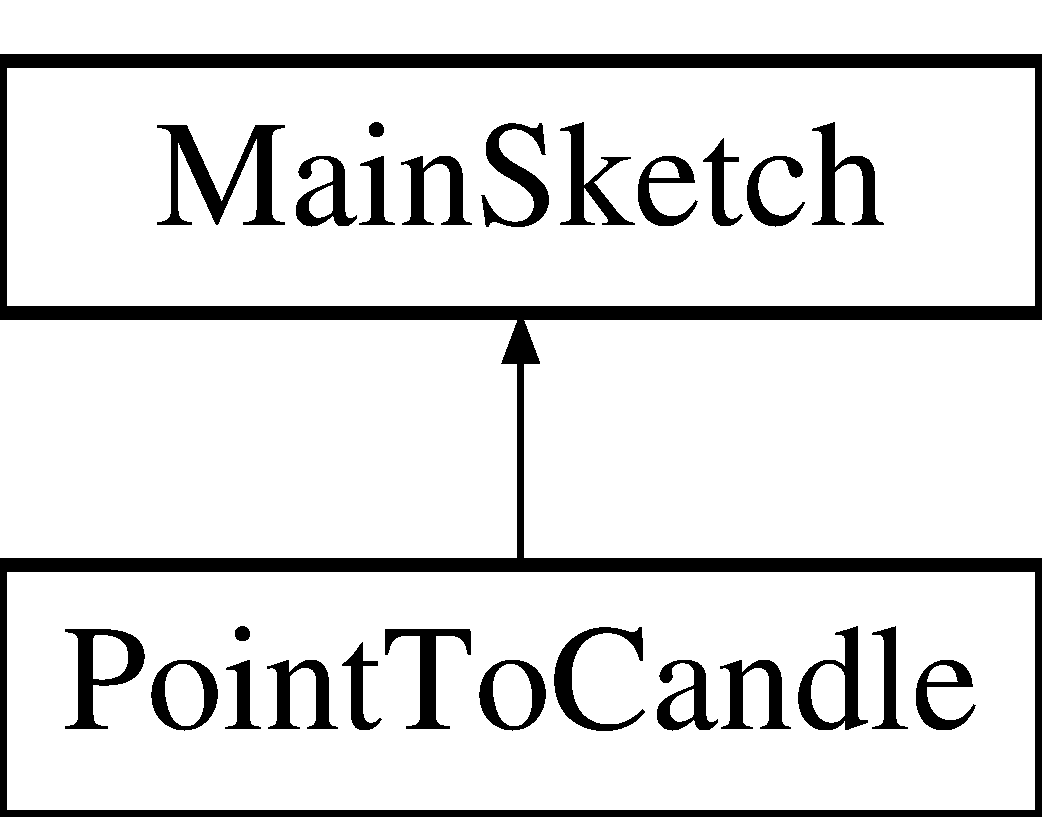
\includegraphics[height=2.000000cm]{classPointToCandle}
\end{center}
\end{figure}
\subsection*{Public Member Functions}
\begin{DoxyCompactItemize}
\item 
void \hyperlink{classPointToCandle_a99ace73720580afda4a41cf01c2418a2}{setup} ()
\begin{DoxyCompactList}\small\item\em pure virtual function for setup. Sublcasses must define \end{DoxyCompactList}\item 
void \hyperlink{classPointToCandle_a446be96046c19b1eff25cf2fcc92ccec}{loop} ()
\begin{DoxyCompactList}\small\item\em pure virtual function for loop. Sublcasses must define \end{DoxyCompactList}\end{DoxyCompactItemize}
\subsection*{Private Member Functions}
\begin{DoxyCompactItemize}
\item 
void \hyperlink{classPointToCandle_a495758f0cc24a3287002d1dd1cdc9698}{turn\-To\-Face} (int angle)
\end{DoxyCompactItemize}
\subsection*{Private Attributes}
\begin{DoxyCompactItemize}
\item 
\hyperlink{classCandleDetector}{Candle\-Detector} \hyperlink{classPointToCandle_a832de7f053912ab631c7f224982bde52}{cd}
\item 
\hyperlink{classLidar}{Lidar} \hyperlink{classPointToCandle_a74def04bd7985f1ae2dfb83cb4ad7d40}{lidar}
\item 
\hyperlink{classDriveMotor}{Drive\-Motor} \hyperlink{classPointToCandle_a8976db9c7a0e1484762bf27c829cb06f}{left}
\item 
\hyperlink{classDriveMotor}{Drive\-Motor} \hyperlink{classPointToCandle_ad0913e5dfa04c7205c16cc893ff238c5}{right}
\item 
int $\ast$ \hyperlink{classPointToCandle_aa905d6ae2cd3d72225020c87f74e30e0}{distances}
\end{DoxyCompactItemize}


\subsection{Detailed Description}


Definition at line 9 of file Point\-To\-Candle.\-hpp.



\subsection{Member Function Documentation}
\hypertarget{classPointToCandle_a446be96046c19b1eff25cf2fcc92ccec}{\index{Point\-To\-Candle@{Point\-To\-Candle}!loop@{loop}}
\index{loop@{loop}!PointToCandle@{Point\-To\-Candle}}
\subsubsection[{loop}]{\setlength{\rightskip}{0pt plus 5cm}void Point\-To\-Candle\-::loop (
\begin{DoxyParamCaption}
{}
\end{DoxyParamCaption}
)\hspace{0.3cm}{\ttfamily [virtual]}}}\label{classPointToCandle_a446be96046c19b1eff25cf2fcc92ccec}


pure virtual function for loop. Sublcasses must define 



Implements \hyperlink{classMainSketch_acd69845de8c794dce73d309f142a6795}{Main\-Sketch}.



Definition at line 30 of file Point\-To\-Candle.\-cpp.

\hypertarget{classPointToCandle_a99ace73720580afda4a41cf01c2418a2}{\index{Point\-To\-Candle@{Point\-To\-Candle}!setup@{setup}}
\index{setup@{setup}!PointToCandle@{Point\-To\-Candle}}
\subsubsection[{setup}]{\setlength{\rightskip}{0pt plus 5cm}void Point\-To\-Candle\-::setup (
\begin{DoxyParamCaption}
{}
\end{DoxyParamCaption}
)\hspace{0.3cm}{\ttfamily [virtual]}}}\label{classPointToCandle_a99ace73720580afda4a41cf01c2418a2}


pure virtual function for setup. Sublcasses must define 



Implements \hyperlink{classMainSketch_a0708e1eb0ced1063f600f4111df90bf2}{Main\-Sketch}.



Definition at line 4 of file Point\-To\-Candle.\-cpp.

\hypertarget{classPointToCandle_a495758f0cc24a3287002d1dd1cdc9698}{\index{Point\-To\-Candle@{Point\-To\-Candle}!turn\-To\-Face@{turn\-To\-Face}}
\index{turn\-To\-Face@{turn\-To\-Face}!PointToCandle@{Point\-To\-Candle}}
\subsubsection[{turn\-To\-Face}]{\setlength{\rightskip}{0pt plus 5cm}void Point\-To\-Candle\-::turn\-To\-Face (
\begin{DoxyParamCaption}
\item[{int}]{angle}
\end{DoxyParamCaption}
)\hspace{0.3cm}{\ttfamily [private]}}}\label{classPointToCandle_a495758f0cc24a3287002d1dd1cdc9698}


Definition at line 10 of file Point\-To\-Candle.\-cpp.



\subsection{Member Data Documentation}
\hypertarget{classPointToCandle_a832de7f053912ab631c7f224982bde52}{\index{Point\-To\-Candle@{Point\-To\-Candle}!cd@{cd}}
\index{cd@{cd}!PointToCandle@{Point\-To\-Candle}}
\subsubsection[{cd}]{\setlength{\rightskip}{0pt plus 5cm}{\bf Candle\-Detector} Point\-To\-Candle\-::cd\hspace{0.3cm}{\ttfamily [private]}}}\label{classPointToCandle_a832de7f053912ab631c7f224982bde52}


Definition at line 17 of file Point\-To\-Candle.\-hpp.

\hypertarget{classPointToCandle_aa905d6ae2cd3d72225020c87f74e30e0}{\index{Point\-To\-Candle@{Point\-To\-Candle}!distances@{distances}}
\index{distances@{distances}!PointToCandle@{Point\-To\-Candle}}
\subsubsection[{distances}]{\setlength{\rightskip}{0pt plus 5cm}int$\ast$ Point\-To\-Candle\-::distances\hspace{0.3cm}{\ttfamily [private]}}}\label{classPointToCandle_aa905d6ae2cd3d72225020c87f74e30e0}


Definition at line 21 of file Point\-To\-Candle.\-hpp.

\hypertarget{classPointToCandle_a8976db9c7a0e1484762bf27c829cb06f}{\index{Point\-To\-Candle@{Point\-To\-Candle}!left@{left}}
\index{left@{left}!PointToCandle@{Point\-To\-Candle}}
\subsubsection[{left}]{\setlength{\rightskip}{0pt plus 5cm}{\bf Drive\-Motor} Point\-To\-Candle\-::left\hspace{0.3cm}{\ttfamily [private]}}}\label{classPointToCandle_a8976db9c7a0e1484762bf27c829cb06f}


Definition at line 19 of file Point\-To\-Candle.\-hpp.

\hypertarget{classPointToCandle_a74def04bd7985f1ae2dfb83cb4ad7d40}{\index{Point\-To\-Candle@{Point\-To\-Candle}!lidar@{lidar}}
\index{lidar@{lidar}!PointToCandle@{Point\-To\-Candle}}
\subsubsection[{lidar}]{\setlength{\rightskip}{0pt plus 5cm}{\bf Lidar} Point\-To\-Candle\-::lidar\hspace{0.3cm}{\ttfamily [private]}}}\label{classPointToCandle_a74def04bd7985f1ae2dfb83cb4ad7d40}


Definition at line 18 of file Point\-To\-Candle.\-hpp.

\hypertarget{classPointToCandle_ad0913e5dfa04c7205c16cc893ff238c5}{\index{Point\-To\-Candle@{Point\-To\-Candle}!right@{right}}
\index{right@{right}!PointToCandle@{Point\-To\-Candle}}
\subsubsection[{right}]{\setlength{\rightskip}{0pt plus 5cm}{\bf Drive\-Motor} Point\-To\-Candle\-::right\hspace{0.3cm}{\ttfamily [private]}}}\label{classPointToCandle_ad0913e5dfa04c7205c16cc893ff238c5}


Definition at line 20 of file Point\-To\-Candle.\-hpp.



The documentation for this class was generated from the following files\-:\begin{DoxyCompactItemize}
\item 
src/test/\hyperlink{PointToCandle_8hpp}{Point\-To\-Candle.\-hpp}\item 
src/test/\hyperlink{PointToCandle_8cpp}{Point\-To\-Candle.\-cpp}\end{DoxyCompactItemize}

\hypertarget{classPrintOdom}{\section{Print\-Odom Class Reference}
\label{classPrintOdom}\index{Print\-Odom@{Print\-Odom}}
}


{\ttfamily \#include $<$Print\-Odom.\-hpp$>$}

Inheritance diagram for Print\-Odom\-:\begin{figure}[H]
\begin{center}
\leavevmode
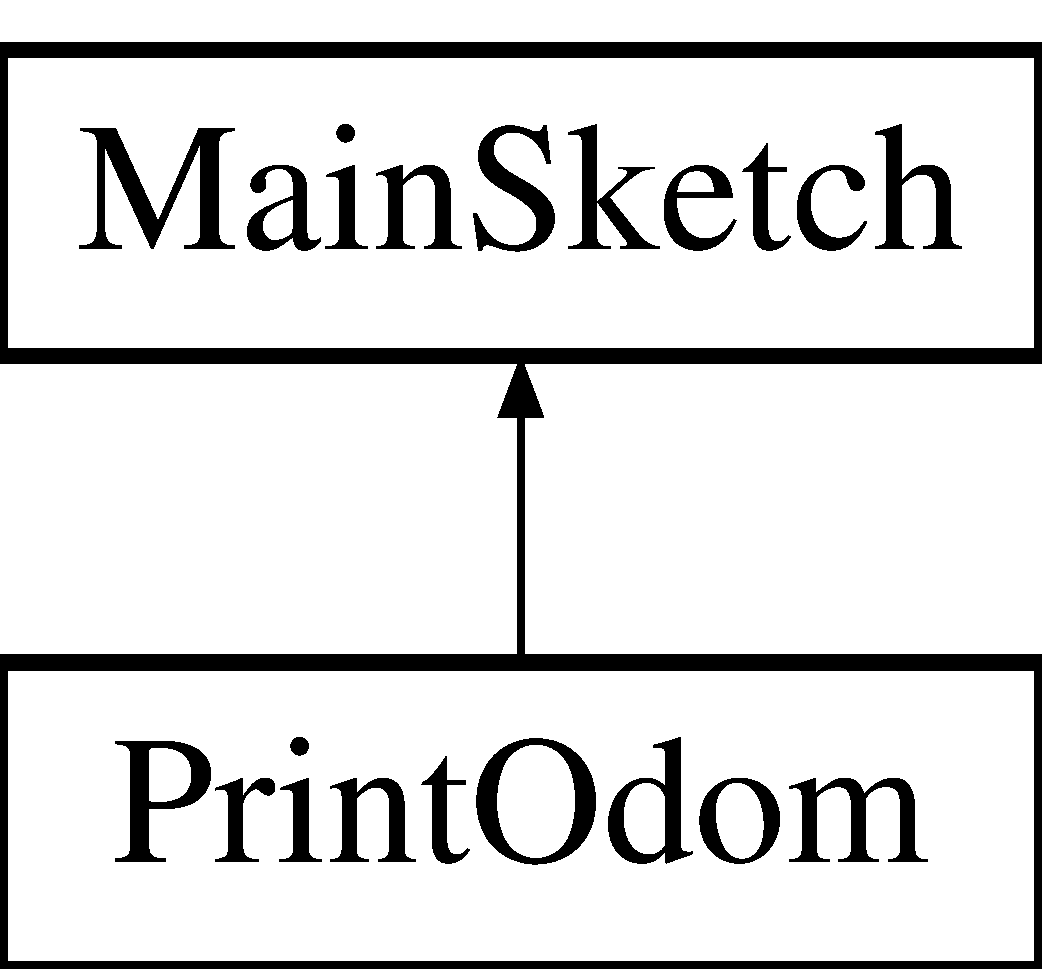
\includegraphics[height=2.000000cm]{classPrintOdom}
\end{center}
\end{figure}
\subsection*{Public Member Functions}
\begin{DoxyCompactItemize}
\item 
void \hyperlink{classPrintOdom_ae99dc882b588ebd47873b7455da5f50a}{setup} ()
\item 
void \hyperlink{classPrintOdom_a4b2515b27a03cb3b143256a52acd5a0c}{loop} ()
\end{DoxyCompactItemize}
\subsection*{Private Types}
\begin{DoxyCompactItemize}
\item 
typedef \hyperlink{classEncoder}{Encoder}$<$ 2, 3 $>$ \hyperlink{classPrintOdom_a6888479f567846e63b00665fe95c4073}{Left\-Enc}
\item 
typedef \hyperlink{classEncoder}{Encoder}$<$ 18, 19 $>$ \hyperlink{classPrintOdom_ac090b58cc7388d8f2e26d5b7c912f383}{Right\-Enc}
\end{DoxyCompactItemize}
\subsection*{Private Attributes}
\begin{DoxyCompactItemize}
\item 
\hyperlink{classOdom}{Odom}$<$ \hyperlink{classPrintOdom_a6888479f567846e63b00665fe95c4073}{Left\-Enc}, \hyperlink{classPrintOdom_ac090b58cc7388d8f2e26d5b7c912f383}{Right\-Enc} $>$ \hyperlink{classPrintOdom_a4741396ec009336b54896ade384b102d}{odom}
\end{DoxyCompactItemize}


\subsection{Detailed Description}


Definition at line 7 of file Print\-Odom.\-hpp.



\subsection{Member Typedef Documentation}
\hypertarget{classPrintOdom_a6888479f567846e63b00665fe95c4073}{\index{Print\-Odom@{Print\-Odom}!Left\-Enc@{Left\-Enc}}
\index{Left\-Enc@{Left\-Enc}!PrintOdom@{Print\-Odom}}
\subsubsection[{Left\-Enc}]{\setlength{\rightskip}{0pt plus 5cm}typedef {\bf Encoder}$<$2,3$>$ {\bf Print\-Odom\-::\-Left\-Enc}\hspace{0.3cm}{\ttfamily [private]}}}\label{classPrintOdom_a6888479f567846e63b00665fe95c4073}


Definition at line 13 of file Print\-Odom.\-hpp.

\hypertarget{classPrintOdom_ac090b58cc7388d8f2e26d5b7c912f383}{\index{Print\-Odom@{Print\-Odom}!Right\-Enc@{Right\-Enc}}
\index{Right\-Enc@{Right\-Enc}!PrintOdom@{Print\-Odom}}
\subsubsection[{Right\-Enc}]{\setlength{\rightskip}{0pt plus 5cm}typedef {\bf Encoder}$<$18,19$>$ {\bf Print\-Odom\-::\-Right\-Enc}\hspace{0.3cm}{\ttfamily [private]}}}\label{classPrintOdom_ac090b58cc7388d8f2e26d5b7c912f383}


Definition at line 14 of file Print\-Odom.\-hpp.



\subsection{Member Function Documentation}
\hypertarget{classPrintOdom_a4b2515b27a03cb3b143256a52acd5a0c}{\index{Print\-Odom@{Print\-Odom}!loop@{loop}}
\index{loop@{loop}!PrintOdom@{Print\-Odom}}
\subsubsection[{loop}]{\setlength{\rightskip}{0pt plus 5cm}void Print\-Odom\-::loop (
\begin{DoxyParamCaption}
{}
\end{DoxyParamCaption}
)\hspace{0.3cm}{\ttfamily [virtual]}}}\label{classPrintOdom_a4b2515b27a03cb3b143256a52acd5a0c}


Implements \hyperlink{classMainSketch_acd69845de8c794dce73d309f142a6795}{Main\-Sketch}.



Definition at line 7 of file Print\-Odom.\-cpp.

\hypertarget{classPrintOdom_ae99dc882b588ebd47873b7455da5f50a}{\index{Print\-Odom@{Print\-Odom}!setup@{setup}}
\index{setup@{setup}!PrintOdom@{Print\-Odom}}
\subsubsection[{setup}]{\setlength{\rightskip}{0pt plus 5cm}void Print\-Odom\-::setup (
\begin{DoxyParamCaption}
{}
\end{DoxyParamCaption}
)\hspace{0.3cm}{\ttfamily [virtual]}}}\label{classPrintOdom_ae99dc882b588ebd47873b7455da5f50a}


Implements \hyperlink{classMainSketch_a0708e1eb0ced1063f600f4111df90bf2}{Main\-Sketch}.



Definition at line 3 of file Print\-Odom.\-cpp.



\subsection{Member Data Documentation}
\hypertarget{classPrintOdom_a4741396ec009336b54896ade384b102d}{\index{Print\-Odom@{Print\-Odom}!odom@{odom}}
\index{odom@{odom}!PrintOdom@{Print\-Odom}}
\subsubsection[{odom}]{\setlength{\rightskip}{0pt plus 5cm}{\bf Odom}$<${\bf Left\-Enc}, {\bf Right\-Enc}$>$ Print\-Odom\-::odom\hspace{0.3cm}{\ttfamily [private]}}}\label{classPrintOdom_a4741396ec009336b54896ade384b102d}


Definition at line 15 of file Print\-Odom.\-hpp.



The documentation for this class was generated from the following files\-:\begin{DoxyCompactItemize}
\item 
src/test/\hyperlink{PrintOdom_8hpp}{Print\-Odom.\-hpp}\item 
src/test/\hyperlink{PrintOdom_8cpp}{Print\-Odom.\-cpp}\end{DoxyCompactItemize}

\hypertarget{classRobot}{\section{Robot Class Reference}
\label{classRobot}\index{Robot@{Robot}}
}


{\ttfamily \#include $<$Robot.\-hpp$>$}

\subsection*{Public Member Functions}
\begin{DoxyCompactItemize}
\item 
void \hyperlink{classRobot_a1fc37e3c329d59795f6adf44199d4df9}{setup} ()
\item 
void \hyperlink{classRobot_a8ad37bfa9e1efeaf7b5eb67667513dbe}{drive} ()
\item 
void \hyperlink{classRobot_a14dfe126ae973d3b9f81fee81a06ac22}{stop} ()
\item 
void \hyperlink{classRobot_ade0935cead03791f27fa854df88a3f22}{set\-Drive} (\hyperlink{DriveMotor_8hpp_a077d9d13989efa3142086ea83cbb1e68}{Drive\-Direction} dir)
\item 
bool \hyperlink{classRobot_a1f08dec6eea6b51d73cd41a8db3bb893}{search} ()
\item 
bool \hyperlink{classRobot_a6b943dfc58f8e1d49ee063250a2621de}{drive\-To\-Candle} ()
\item 
bool \hyperlink{classRobot_a17e0de9c529197b3575e11a87470376b}{find\-Candle\-Height} ()
\item 
bool \hyperlink{classRobot_a0dfb8f97d6a9448bc6f9ccc5b9efb9fb}{extinguish\-Candle} ()
\item 
bool \hyperlink{classRobot_ac1faa7fbfb483c4053dc35f368359c0b}{return\-To\-Origin} ()
\item 
bool \hyperlink{classRobot_afa750c4ecf35e5f26992779ac89eb13e}{turn\-To\-Face} (int angle)
\item 
void \hyperlink{classRobot_ae7a44c77eacc2a9a3d41f7a18cfb401f}{drive\-And\-Avoid} ()
\end{DoxyCompactItemize}
\subsection*{Static Public Member Functions}
\begin{DoxyCompactItemize}
\item 
static \hyperlink{classRobot}{Robot} $\ast$ \hyperlink{classRobot_ac6f19dc31b435f8a2d43944ba49286d0}{get\-Instance} ()
\end{DoxyCompactItemize}
\subsection*{Public Attributes}
\begin{DoxyCompactItemize}
\item 
\hyperlink{classLidar}{Lidar} \hyperlink{classRobot_a222e54f477e23f5af80cfa10bcd85e7a}{lidar}
\item 
\hyperlink{classPIDBase}{P\-I\-D\-Base} \hyperlink{classRobot_adbf538f97c0f9f98337f5171e715badc}{base}
\end{DoxyCompactItemize}
\subsection*{Private Member Functions}
\begin{DoxyCompactItemize}
\item 
\hyperlink{classRobot_a4fc7c70ae20623f05e06f2ecb388b6c4}{Robot} ()
\end{DoxyCompactItemize}
\subsection*{Private Attributes}
\begin{DoxyCompactItemize}
\item 
\hyperlink{classSearcher}{Searcher} \hyperlink{classRobot_af0ba30c47b84dc976f5bb7bd978f95ef}{searcher}
\item 
\hyperlink{DriveMotor_8hpp_a077d9d13989efa3142086ea83cbb1e68}{Drive\-Direction} \hyperlink{classRobot_af15d2eaa46a9736e5d3d3aa9e8a9751c}{drive\-Direction}
\item 
\hyperlink{classCandleDetector}{Candle\-Detector} \hyperlink{classRobot_a19cb4c2ee87b595db9275e6b3d9ca30d}{detector}
\item 
\hyperlink{classFireFinder}{Fire\-Finder} \hyperlink{classRobot_a342f5f8be2b5641eb3ae8f9c8475ebe6}{ff}
\item 
int $\ast$ \hyperlink{classRobot_aba9dccea96aa95bb8fbdd1a5ba72ca73}{distances}
\item 
int \hyperlink{classRobot_afae387e4e9419530d3217055301ba939}{distance\-To\-Candle}
\item 
int \hyperlink{classRobot_a7c1bd342087a6eedeeb0df07fa9cf3d2}{angle\-To\-Candle}
\end{DoxyCompactItemize}
\subsection*{Static Private Attributes}
\begin{DoxyCompactItemize}
\item 
static \hyperlink{classRobot}{Robot} $\ast$ \hyperlink{classRobot_aad5c5d6db601aac62393d47ec9385fa3}{instance} = N\-U\-L\-L
\item 
static const int \hyperlink{classRobot_afb4449356b3a3f92b2c76c612e8951ee}{G\-O\-A\-L\-\_\-\-D\-I\-S\-T\-A\-N\-C\-E} = 300
\end{DoxyCompactItemize}


\subsection{Detailed Description}


Definition at line 10 of file Robot.\-hpp.



\subsection{Constructor \& Destructor Documentation}
\hypertarget{classRobot_a4fc7c70ae20623f05e06f2ecb388b6c4}{\index{Robot@{Robot}!Robot@{Robot}}
\index{Robot@{Robot}!Robot@{Robot}}
\subsubsection[{Robot}]{\setlength{\rightskip}{0pt plus 5cm}Robot\-::\-Robot (
\begin{DoxyParamCaption}
{}
\end{DoxyParamCaption}
)\hspace{0.3cm}{\ttfamily [private]}}}\label{classRobot_a4fc7c70ae20623f05e06f2ecb388b6c4}
constructor is private because it's a singleton class 

Definition at line 7 of file Robot.\-cpp.



\subsection{Member Function Documentation}
\hypertarget{classRobot_a8ad37bfa9e1efeaf7b5eb67667513dbe}{\index{Robot@{Robot}!drive@{drive}}
\index{drive@{drive}!Robot@{Robot}}
\subsubsection[{drive}]{\setlength{\rightskip}{0pt plus 5cm}void Robot\-::drive (
\begin{DoxyParamCaption}
{}
\end{DoxyParamCaption}
)}}\label{classRobot_a8ad37bfa9e1efeaf7b5eb67667513dbe}


Definition at line 23 of file Robot.\-cpp.

\hypertarget{classRobot_ae7a44c77eacc2a9a3d41f7a18cfb401f}{\index{Robot@{Robot}!drive\-And\-Avoid@{drive\-And\-Avoid}}
\index{drive\-And\-Avoid@{drive\-And\-Avoid}!Robot@{Robot}}
\subsubsection[{drive\-And\-Avoid}]{\setlength{\rightskip}{0pt plus 5cm}void Robot\-::drive\-And\-Avoid (
\begin{DoxyParamCaption}
{}
\end{DoxyParamCaption}
)}}\label{classRobot_ae7a44c77eacc2a9a3d41f7a18cfb401f}


Definition at line 117 of file Robot.\-cpp.

\hypertarget{classRobot_a6b943dfc58f8e1d49ee063250a2621de}{\index{Robot@{Robot}!drive\-To\-Candle@{drive\-To\-Candle}}
\index{drive\-To\-Candle@{drive\-To\-Candle}!Robot@{Robot}}
\subsubsection[{drive\-To\-Candle}]{\setlength{\rightskip}{0pt plus 5cm}bool Robot\-::drive\-To\-Candle (
\begin{DoxyParamCaption}
{}
\end{DoxyParamCaption}
)}}\label{classRobot_a6b943dfc58f8e1d49ee063250a2621de}


Definition at line 69 of file Robot.\-cpp.

\hypertarget{classRobot_a0dfb8f97d6a9448bc6f9ccc5b9efb9fb}{\index{Robot@{Robot}!extinguish\-Candle@{extinguish\-Candle}}
\index{extinguish\-Candle@{extinguish\-Candle}!Robot@{Robot}}
\subsubsection[{extinguish\-Candle}]{\setlength{\rightskip}{0pt plus 5cm}bool Robot\-::extinguish\-Candle (
\begin{DoxyParamCaption}
{}
\end{DoxyParamCaption}
)}}\label{classRobot_a0dfb8f97d6a9448bc6f9ccc5b9efb9fb}


Definition at line 86 of file Robot.\-cpp.

\hypertarget{classRobot_a17e0de9c529197b3575e11a87470376b}{\index{Robot@{Robot}!find\-Candle\-Height@{find\-Candle\-Height}}
\index{find\-Candle\-Height@{find\-Candle\-Height}!Robot@{Robot}}
\subsubsection[{find\-Candle\-Height}]{\setlength{\rightskip}{0pt plus 5cm}bool Robot\-::find\-Candle\-Height (
\begin{DoxyParamCaption}
{}
\end{DoxyParamCaption}
)}}\label{classRobot_a17e0de9c529197b3575e11a87470376b}


Definition at line 81 of file Robot.\-cpp.

\hypertarget{classRobot_ac6f19dc31b435f8a2d43944ba49286d0}{\index{Robot@{Robot}!get\-Instance@{get\-Instance}}
\index{get\-Instance@{get\-Instance}!Robot@{Robot}}
\subsubsection[{get\-Instance}]{\setlength{\rightskip}{0pt plus 5cm}{\bf Robot} $\ast$ Robot\-::get\-Instance (
\begin{DoxyParamCaption}
{}
\end{DoxyParamCaption}
)\hspace{0.3cm}{\ttfamily [static]}}}\label{classRobot_ac6f19dc31b435f8a2d43944ba49286d0}


Definition at line 15 of file Robot.\-cpp.

\hypertarget{classRobot_ac1faa7fbfb483c4053dc35f368359c0b}{\index{Robot@{Robot}!return\-To\-Origin@{return\-To\-Origin}}
\index{return\-To\-Origin@{return\-To\-Origin}!Robot@{Robot}}
\subsubsection[{return\-To\-Origin}]{\setlength{\rightskip}{0pt plus 5cm}bool Robot\-::return\-To\-Origin (
\begin{DoxyParamCaption}
{}
\end{DoxyParamCaption}
)}}\label{classRobot_ac1faa7fbfb483c4053dc35f368359c0b}


Definition at line 90 of file Robot.\-cpp.

\hypertarget{classRobot_a1f08dec6eea6b51d73cd41a8db3bb893}{\index{Robot@{Robot}!search@{search}}
\index{search@{search}!Robot@{Robot}}
\subsubsection[{search}]{\setlength{\rightskip}{0pt plus 5cm}bool Robot\-::search (
\begin{DoxyParamCaption}
{}
\end{DoxyParamCaption}
)}}\label{classRobot_a1f08dec6eea6b51d73cd41a8db3bb893}
search for candle by driving around \begin{DoxyReturn}{Returns}
true when the candle has been found 
\end{DoxyReturn}


Definition at line 53 of file Robot.\-cpp.

\hypertarget{classRobot_ade0935cead03791f27fa854df88a3f22}{\index{Robot@{Robot}!set\-Drive@{set\-Drive}}
\index{set\-Drive@{set\-Drive}!Robot@{Robot}}
\subsubsection[{set\-Drive}]{\setlength{\rightskip}{0pt plus 5cm}void Robot\-::set\-Drive (
\begin{DoxyParamCaption}
\item[{{\bf Drive\-Direction}}]{dir}
\end{DoxyParamCaption}
)}}\label{classRobot_ade0935cead03791f27fa854df88a3f22}
given a direction, set the motor P\-I\-Ds accordingly 
\begin{DoxyParams}{Parameters}
{\em dir} & the direction you want to go \\
\hline
\end{DoxyParams}


Definition at line 49 of file Robot.\-cpp.

\hypertarget{classRobot_a1fc37e3c329d59795f6adf44199d4df9}{\index{Robot@{Robot}!setup@{setup}}
\index{setup@{setup}!Robot@{Robot}}
\subsubsection[{setup}]{\setlength{\rightskip}{0pt plus 5cm}void Robot\-::setup (
\begin{DoxyParamCaption}
{}
\end{DoxyParamCaption}
)}}\label{classRobot_a1fc37e3c329d59795f6adf44199d4df9}


Definition at line 9 of file Robot.\-cpp.

\hypertarget{classRobot_a14dfe126ae973d3b9f81fee81a06ac22}{\index{Robot@{Robot}!stop@{stop}}
\index{stop@{stop}!Robot@{Robot}}
\subsubsection[{stop}]{\setlength{\rightskip}{0pt plus 5cm}void Robot\-::stop (
\begin{DoxyParamCaption}
{}
\end{DoxyParamCaption}
)}}\label{classRobot_a14dfe126ae973d3b9f81fee81a06ac22}


Definition at line 45 of file Robot.\-cpp.

\hypertarget{classRobot_afa750c4ecf35e5f26992779ac89eb13e}{\index{Robot@{Robot}!turn\-To\-Face@{turn\-To\-Face}}
\index{turn\-To\-Face@{turn\-To\-Face}!Robot@{Robot}}
\subsubsection[{turn\-To\-Face}]{\setlength{\rightskip}{0pt plus 5cm}bool Robot\-::turn\-To\-Face (
\begin{DoxyParamCaption}
\item[{int}]{angle}
\end{DoxyParamCaption}
)}}\label{classRobot_afa750c4ecf35e5f26992779ac89eb13e}


Definition at line 94 of file Robot.\-cpp.



\subsection{Member Data Documentation}
\hypertarget{classRobot_a7c1bd342087a6eedeeb0df07fa9cf3d2}{\index{Robot@{Robot}!angle\-To\-Candle@{angle\-To\-Candle}}
\index{angle\-To\-Candle@{angle\-To\-Candle}!Robot@{Robot}}
\subsubsection[{angle\-To\-Candle}]{\setlength{\rightskip}{0pt plus 5cm}int Robot\-::angle\-To\-Candle\hspace{0.3cm}{\ttfamily [private]}}}\label{classRobot_a7c1bd342087a6eedeeb0df07fa9cf3d2}


Definition at line 59 of file Robot.\-hpp.

\hypertarget{classRobot_adbf538f97c0f9f98337f5171e715badc}{\index{Robot@{Robot}!base@{base}}
\index{base@{base}!Robot@{Robot}}
\subsubsection[{base}]{\setlength{\rightskip}{0pt plus 5cm}{\bf P\-I\-D\-Base} Robot\-::base}}\label{classRobot_adbf538f97c0f9f98337f5171e715badc}


Definition at line 44 of file Robot.\-hpp.

\hypertarget{classRobot_a19cb4c2ee87b595db9275e6b3d9ca30d}{\index{Robot@{Robot}!detector@{detector}}
\index{detector@{detector}!Robot@{Robot}}
\subsubsection[{detector}]{\setlength{\rightskip}{0pt plus 5cm}{\bf Candle\-Detector} Robot\-::detector\hspace{0.3cm}{\ttfamily [private]}}}\label{classRobot_a19cb4c2ee87b595db9275e6b3d9ca30d}


Definition at line 54 of file Robot.\-hpp.

\hypertarget{classRobot_aba9dccea96aa95bb8fbdd1a5ba72ca73}{\index{Robot@{Robot}!distances@{distances}}
\index{distances@{distances}!Robot@{Robot}}
\subsubsection[{distances}]{\setlength{\rightskip}{0pt plus 5cm}int$\ast$ Robot\-::distances\hspace{0.3cm}{\ttfamily [private]}}}\label{classRobot_aba9dccea96aa95bb8fbdd1a5ba72ca73}


Definition at line 57 of file Robot.\-hpp.

\hypertarget{classRobot_afae387e4e9419530d3217055301ba939}{\index{Robot@{Robot}!distance\-To\-Candle@{distance\-To\-Candle}}
\index{distance\-To\-Candle@{distance\-To\-Candle}!Robot@{Robot}}
\subsubsection[{distance\-To\-Candle}]{\setlength{\rightskip}{0pt plus 5cm}int Robot\-::distance\-To\-Candle\hspace{0.3cm}{\ttfamily [private]}}}\label{classRobot_afae387e4e9419530d3217055301ba939}


Definition at line 58 of file Robot.\-hpp.

\hypertarget{classRobot_af15d2eaa46a9736e5d3d3aa9e8a9751c}{\index{Robot@{Robot}!drive\-Direction@{drive\-Direction}}
\index{drive\-Direction@{drive\-Direction}!Robot@{Robot}}
\subsubsection[{drive\-Direction}]{\setlength{\rightskip}{0pt plus 5cm}{\bf Drive\-Direction} Robot\-::drive\-Direction\hspace{0.3cm}{\ttfamily [private]}}}\label{classRobot_af15d2eaa46a9736e5d3d3aa9e8a9751c}


Definition at line 53 of file Robot.\-hpp.

\hypertarget{classRobot_a342f5f8be2b5641eb3ae8f9c8475ebe6}{\index{Robot@{Robot}!ff@{ff}}
\index{ff@{ff}!Robot@{Robot}}
\subsubsection[{ff}]{\setlength{\rightskip}{0pt plus 5cm}{\bf Fire\-Finder} Robot\-::ff\hspace{0.3cm}{\ttfamily [private]}}}\label{classRobot_a342f5f8be2b5641eb3ae8f9c8475ebe6}


Definition at line 55 of file Robot.\-hpp.

\hypertarget{classRobot_afb4449356b3a3f92b2c76c612e8951ee}{\index{Robot@{Robot}!G\-O\-A\-L\-\_\-\-D\-I\-S\-T\-A\-N\-C\-E@{G\-O\-A\-L\-\_\-\-D\-I\-S\-T\-A\-N\-C\-E}}
\index{G\-O\-A\-L\-\_\-\-D\-I\-S\-T\-A\-N\-C\-E@{G\-O\-A\-L\-\_\-\-D\-I\-S\-T\-A\-N\-C\-E}!Robot@{Robot}}
\subsubsection[{G\-O\-A\-L\-\_\-\-D\-I\-S\-T\-A\-N\-C\-E}]{\setlength{\rightskip}{0pt plus 5cm}const int Robot\-::\-G\-O\-A\-L\-\_\-\-D\-I\-S\-T\-A\-N\-C\-E = 300\hspace{0.3cm}{\ttfamily [static]}, {\ttfamily [private]}}}\label{classRobot_afb4449356b3a3f92b2c76c612e8951ee}


Definition at line 61 of file Robot.\-hpp.

\hypertarget{classRobot_aad5c5d6db601aac62393d47ec9385fa3}{\index{Robot@{Robot}!instance@{instance}}
\index{instance@{instance}!Robot@{Robot}}
\subsubsection[{instance}]{\setlength{\rightskip}{0pt plus 5cm}{\bf Robot} $\ast$ Robot\-::instance = N\-U\-L\-L\hspace{0.3cm}{\ttfamily [static]}, {\ttfamily [private]}}}\label{classRobot_aad5c5d6db601aac62393d47ec9385fa3}


Definition at line 50 of file Robot.\-hpp.

\hypertarget{classRobot_a222e54f477e23f5af80cfa10bcd85e7a}{\index{Robot@{Robot}!lidar@{lidar}}
\index{lidar@{lidar}!Robot@{Robot}}
\subsubsection[{lidar}]{\setlength{\rightskip}{0pt plus 5cm}{\bf Lidar} Robot\-::lidar}}\label{classRobot_a222e54f477e23f5af80cfa10bcd85e7a}
making these public so other subsystems (candle) 

Definition at line 43 of file Robot.\-hpp.

\hypertarget{classRobot_af0ba30c47b84dc976f5bb7bd978f95ef}{\index{Robot@{Robot}!searcher@{searcher}}
\index{searcher@{searcher}!Robot@{Robot}}
\subsubsection[{searcher}]{\setlength{\rightskip}{0pt plus 5cm}{\bf Searcher} Robot\-::searcher\hspace{0.3cm}{\ttfamily [private]}}}\label{classRobot_af0ba30c47b84dc976f5bb7bd978f95ef}


Definition at line 52 of file Robot.\-hpp.



The documentation for this class was generated from the following files\-:\begin{DoxyCompactItemize}
\item 
src/test/\hyperlink{Robot_8hpp}{Robot.\-hpp}\item 
src/test/\hyperlink{Robot_8cpp}{Robot.\-cpp}\end{DoxyCompactItemize}

\hypertarget{classSearch}{\section{Search Class Reference}
\label{classSearch}\index{Search@{Search}}
}


{\ttfamily \#include $<$Search.\-hpp$>$}

Inheritance diagram for Search\-:\begin{figure}[H]
\begin{center}
\leavevmode
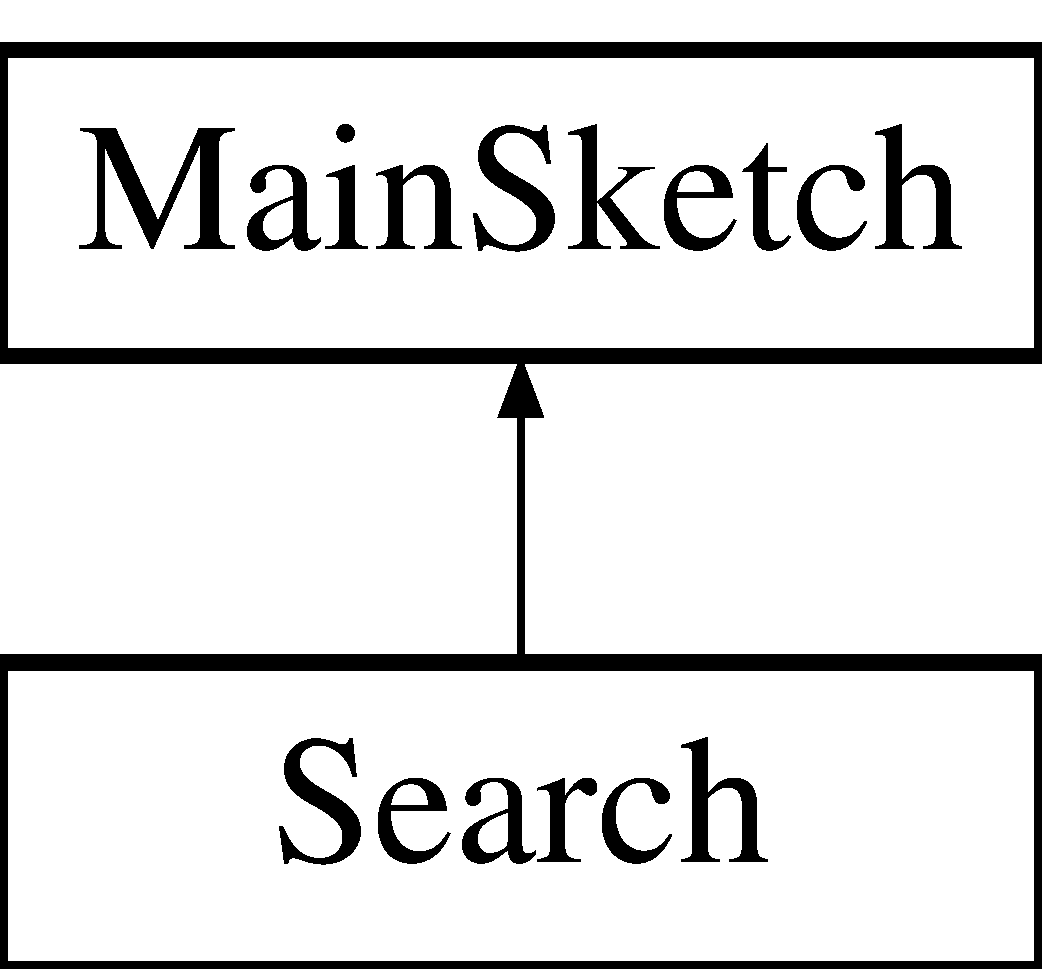
\includegraphics[height=2.000000cm]{classSearch}
\end{center}
\end{figure}
\subsection*{Public Member Functions}
\begin{DoxyCompactItemize}
\item 
void \hyperlink{classSearch_ad5de8c844478b7f0903d724236fd12ad}{setup} ()
\item 
void \hyperlink{classSearch_a75f9358f4551ee9ed0d750eac8fd479e}{loop} ()
\end{DoxyCompactItemize}
\subsection*{Private Attributes}
\begin{DoxyCompactItemize}
\item 
\hyperlink{classLidar}{Lidar} \hyperlink{classSearch_ad1209571d5e6cb4c53494549d8ec4ac6}{lidar}
\item 
\hyperlink{classDriveMotor}{Drive\-Motor} \hyperlink{classSearch_ad1df1ee1c5afbeb2767a4c1e064e7318}{left}
\item 
\hyperlink{classDriveMotor}{Drive\-Motor} \hyperlink{classSearch_a7f0e23cc5c8aa635fbe7f5b4c8e30eb0}{right}
\item 
int $\ast$ \hyperlink{classSearch_acae7260fec1cd49350860f94955b1e63}{distances}
\item 
bool \hyperlink{classSearch_aef5f5e911426d02067e2ac01e5549f1e}{turning} = false
\item 
int \hyperlink{classSearch_a443c7d18e6cfd0d114f7e2c2b1495bec}{d\-Front}
\item 
int \hyperlink{classSearch_a376def82b93387197752cc169ddf060e}{d\-Right}
\item 
int \hyperlink{classSearch_aeab525e9821cdb2dc5ed996a207d9084}{d\-Left}
\item 
long \hyperlink{classSearch_ac5a0e7842cdfec65c8af8fd2dd0d4dcc}{last\-\_\-update}
\item 
long \hyperlink{classSearch_af73bd725381f47afa3bf6af64d39f3b6}{last\-Motor\-Loop}
\item 
bool \hyperlink{classSearch_a113ce5d7076372bbe5041749f42a7ee3}{full\-Sweep}
\end{DoxyCompactItemize}


\subsection{Detailed Description}


Definition at line 8 of file Search.\-hpp.



\subsection{Member Function Documentation}
\hypertarget{classSearch_a75f9358f4551ee9ed0d750eac8fd479e}{\index{Search@{Search}!loop@{loop}}
\index{loop@{loop}!Search@{Search}}
\subsubsection[{loop}]{\setlength{\rightskip}{0pt plus 5cm}void Search\-::loop (
\begin{DoxyParamCaption}
{}
\end{DoxyParamCaption}
)\hspace{0.3cm}{\ttfamily [virtual]}}}\label{classSearch_a75f9358f4551ee9ed0d750eac8fd479e}


Implements \hyperlink{classMainSketch_acd69845de8c794dce73d309f142a6795}{Main\-Sketch}.



Definition at line 12 of file Search.\-cpp.

\hypertarget{classSearch_ad5de8c844478b7f0903d724236fd12ad}{\index{Search@{Search}!setup@{setup}}
\index{setup@{setup}!Search@{Search}}
\subsubsection[{setup}]{\setlength{\rightskip}{0pt plus 5cm}void Search\-::setup (
\begin{DoxyParamCaption}
{}
\end{DoxyParamCaption}
)\hspace{0.3cm}{\ttfamily [virtual]}}}\label{classSearch_ad5de8c844478b7f0903d724236fd12ad}


Implements \hyperlink{classMainSketch_a0708e1eb0ced1063f600f4111df90bf2}{Main\-Sketch}.



Definition at line 4 of file Search.\-cpp.



\subsection{Member Data Documentation}
\hypertarget{classSearch_a443c7d18e6cfd0d114f7e2c2b1495bec}{\index{Search@{Search}!d\-Front@{d\-Front}}
\index{d\-Front@{d\-Front}!Search@{Search}}
\subsubsection[{d\-Front}]{\setlength{\rightskip}{0pt plus 5cm}int Search\-::d\-Front\hspace{0.3cm}{\ttfamily [private]}}}\label{classSearch_a443c7d18e6cfd0d114f7e2c2b1495bec}


Definition at line 19 of file Search.\-hpp.

\hypertarget{classSearch_acae7260fec1cd49350860f94955b1e63}{\index{Search@{Search}!distances@{distances}}
\index{distances@{distances}!Search@{Search}}
\subsubsection[{distances}]{\setlength{\rightskip}{0pt plus 5cm}int$\ast$ Search\-::distances\hspace{0.3cm}{\ttfamily [private]}}}\label{classSearch_acae7260fec1cd49350860f94955b1e63}


Definition at line 17 of file Search.\-hpp.

\hypertarget{classSearch_aeab525e9821cdb2dc5ed996a207d9084}{\index{Search@{Search}!d\-Left@{d\-Left}}
\index{d\-Left@{d\-Left}!Search@{Search}}
\subsubsection[{d\-Left}]{\setlength{\rightskip}{0pt plus 5cm}int Search\-::d\-Left\hspace{0.3cm}{\ttfamily [private]}}}\label{classSearch_aeab525e9821cdb2dc5ed996a207d9084}


Definition at line 19 of file Search.\-hpp.

\hypertarget{classSearch_a376def82b93387197752cc169ddf060e}{\index{Search@{Search}!d\-Right@{d\-Right}}
\index{d\-Right@{d\-Right}!Search@{Search}}
\subsubsection[{d\-Right}]{\setlength{\rightskip}{0pt plus 5cm}int Search\-::d\-Right\hspace{0.3cm}{\ttfamily [private]}}}\label{classSearch_a376def82b93387197752cc169ddf060e}


Definition at line 19 of file Search.\-hpp.

\hypertarget{classSearch_a113ce5d7076372bbe5041749f42a7ee3}{\index{Search@{Search}!full\-Sweep@{full\-Sweep}}
\index{full\-Sweep@{full\-Sweep}!Search@{Search}}
\subsubsection[{full\-Sweep}]{\setlength{\rightskip}{0pt plus 5cm}bool Search\-::full\-Sweep\hspace{0.3cm}{\ttfamily [private]}}}\label{classSearch_a113ce5d7076372bbe5041749f42a7ee3}


Definition at line 21 of file Search.\-hpp.

\hypertarget{classSearch_ac5a0e7842cdfec65c8af8fd2dd0d4dcc}{\index{Search@{Search}!last\-\_\-update@{last\-\_\-update}}
\index{last\-\_\-update@{last\-\_\-update}!Search@{Search}}
\subsubsection[{last\-\_\-update}]{\setlength{\rightskip}{0pt plus 5cm}long Search\-::last\-\_\-update\hspace{0.3cm}{\ttfamily [private]}}}\label{classSearch_ac5a0e7842cdfec65c8af8fd2dd0d4dcc}


Definition at line 20 of file Search.\-hpp.

\hypertarget{classSearch_af73bd725381f47afa3bf6af64d39f3b6}{\index{Search@{Search}!last\-Motor\-Loop@{last\-Motor\-Loop}}
\index{last\-Motor\-Loop@{last\-Motor\-Loop}!Search@{Search}}
\subsubsection[{last\-Motor\-Loop}]{\setlength{\rightskip}{0pt plus 5cm}long Search\-::last\-Motor\-Loop\hspace{0.3cm}{\ttfamily [private]}}}\label{classSearch_af73bd725381f47afa3bf6af64d39f3b6}


Definition at line 20 of file Search.\-hpp.

\hypertarget{classSearch_ad1df1ee1c5afbeb2767a4c1e064e7318}{\index{Search@{Search}!left@{left}}
\index{left@{left}!Search@{Search}}
\subsubsection[{left}]{\setlength{\rightskip}{0pt plus 5cm}{\bf Drive\-Motor} Search\-::left\hspace{0.3cm}{\ttfamily [private]}}}\label{classSearch_ad1df1ee1c5afbeb2767a4c1e064e7318}


Definition at line 15 of file Search.\-hpp.

\hypertarget{classSearch_ad1209571d5e6cb4c53494549d8ec4ac6}{\index{Search@{Search}!lidar@{lidar}}
\index{lidar@{lidar}!Search@{Search}}
\subsubsection[{lidar}]{\setlength{\rightskip}{0pt plus 5cm}{\bf Lidar} Search\-::lidar\hspace{0.3cm}{\ttfamily [private]}}}\label{classSearch_ad1209571d5e6cb4c53494549d8ec4ac6}


Definition at line 14 of file Search.\-hpp.

\hypertarget{classSearch_a7f0e23cc5c8aa635fbe7f5b4c8e30eb0}{\index{Search@{Search}!right@{right}}
\index{right@{right}!Search@{Search}}
\subsubsection[{right}]{\setlength{\rightskip}{0pt plus 5cm}{\bf Drive\-Motor} Search\-::right\hspace{0.3cm}{\ttfamily [private]}}}\label{classSearch_a7f0e23cc5c8aa635fbe7f5b4c8e30eb0}


Definition at line 16 of file Search.\-hpp.

\hypertarget{classSearch_aef5f5e911426d02067e2ac01e5549f1e}{\index{Search@{Search}!turning@{turning}}
\index{turning@{turning}!Search@{Search}}
\subsubsection[{turning}]{\setlength{\rightskip}{0pt plus 5cm}bool Search\-::turning = false\hspace{0.3cm}{\ttfamily [private]}}}\label{classSearch_aef5f5e911426d02067e2ac01e5549f1e}


Definition at line 18 of file Search.\-hpp.



The documentation for this class was generated from the following files\-:\begin{DoxyCompactItemize}
\item 
src/test/\hyperlink{Search_8hpp}{Search.\-hpp}\item 
src/test/\hyperlink{Search_8cpp}{Search.\-cpp}\end{DoxyCompactItemize}

\hypertarget{classSearcher}{\section{Searcher Class Reference}
\label{classSearcher}\index{Searcher@{Searcher}}
}


{\ttfamily \#include $<$Searcher.\-hpp$>$}

\subsection*{Public Member Functions}
\begin{DoxyCompactItemize}
\item 
\hyperlink{DriveMotor_8hpp_a077d9d13989efa3142086ea83cbb1e68}{Drive\-Direction} \hyperlink{classSearcher_a9ef68e37a381056db7ed4f119b472719}{get\-Direction} ()
\end{DoxyCompactItemize}
\subsection*{Private Attributes}
\begin{DoxyCompactItemize}
\item 
bool \hyperlink{classSearcher_aa1764fe370476e6bf19b30e5a8c2b073}{turning} = false
\item 
int \hyperlink{classSearcher_ae9ecf25b0705199abad716431659d4b6}{d\-Front}
\item 
int \hyperlink{classSearcher_a56c7e8eb20ba293376d59dc55ac4a0c5}{d\-Right}
\item 
int \hyperlink{classSearcher_afa55bd372a5cb9cdebc9720dfe098e4d}{d\-Left}
\item 
float \hyperlink{classSearcher_af6082983203ee203e741b79737c205d6}{last\-Direction}
\item 
bool \hyperlink{classSearcher_a34cdc6cbf4aa91ade07e1b9e5aa362fb}{full\-Sweep}
\end{DoxyCompactItemize}


\subsection{Detailed Description}


Definition at line 6 of file Searcher.\-hpp.



\subsection{Member Function Documentation}
\hypertarget{classSearcher_a9ef68e37a381056db7ed4f119b472719}{\index{Searcher@{Searcher}!get\-Direction@{get\-Direction}}
\index{get\-Direction@{get\-Direction}!Searcher@{Searcher}}
\subsubsection[{get\-Direction}]{\setlength{\rightskip}{0pt plus 5cm}{\bf Drive\-Direction} Searcher\-::get\-Direction (
\begin{DoxyParamCaption}
{}
\end{DoxyParamCaption}
)}}\label{classSearcher_a9ef68e37a381056db7ed4f119b472719}


Definition at line 5 of file Searcher.\-cpp.



\subsection{Member Data Documentation}
\hypertarget{classSearcher_ae9ecf25b0705199abad716431659d4b6}{\index{Searcher@{Searcher}!d\-Front@{d\-Front}}
\index{d\-Front@{d\-Front}!Searcher@{Searcher}}
\subsubsection[{d\-Front}]{\setlength{\rightskip}{0pt plus 5cm}int Searcher\-::d\-Front\hspace{0.3cm}{\ttfamily [private]}}}\label{classSearcher_ae9ecf25b0705199abad716431659d4b6}


Definition at line 12 of file Searcher.\-hpp.

\hypertarget{classSearcher_afa55bd372a5cb9cdebc9720dfe098e4d}{\index{Searcher@{Searcher}!d\-Left@{d\-Left}}
\index{d\-Left@{d\-Left}!Searcher@{Searcher}}
\subsubsection[{d\-Left}]{\setlength{\rightskip}{0pt plus 5cm}int Searcher\-::d\-Left\hspace{0.3cm}{\ttfamily [private]}}}\label{classSearcher_afa55bd372a5cb9cdebc9720dfe098e4d}


Definition at line 12 of file Searcher.\-hpp.

\hypertarget{classSearcher_a56c7e8eb20ba293376d59dc55ac4a0c5}{\index{Searcher@{Searcher}!d\-Right@{d\-Right}}
\index{d\-Right@{d\-Right}!Searcher@{Searcher}}
\subsubsection[{d\-Right}]{\setlength{\rightskip}{0pt plus 5cm}int Searcher\-::d\-Right\hspace{0.3cm}{\ttfamily [private]}}}\label{classSearcher_a56c7e8eb20ba293376d59dc55ac4a0c5}


Definition at line 12 of file Searcher.\-hpp.

\hypertarget{classSearcher_a34cdc6cbf4aa91ade07e1b9e5aa362fb}{\index{Searcher@{Searcher}!full\-Sweep@{full\-Sweep}}
\index{full\-Sweep@{full\-Sweep}!Searcher@{Searcher}}
\subsubsection[{full\-Sweep}]{\setlength{\rightskip}{0pt plus 5cm}bool Searcher\-::full\-Sweep\hspace{0.3cm}{\ttfamily [private]}}}\label{classSearcher_a34cdc6cbf4aa91ade07e1b9e5aa362fb}


Definition at line 14 of file Searcher.\-hpp.

\hypertarget{classSearcher_af6082983203ee203e741b79737c205d6}{\index{Searcher@{Searcher}!last\-Direction@{last\-Direction}}
\index{last\-Direction@{last\-Direction}!Searcher@{Searcher}}
\subsubsection[{last\-Direction}]{\setlength{\rightskip}{0pt plus 5cm}float Searcher\-::last\-Direction\hspace{0.3cm}{\ttfamily [private]}}}\label{classSearcher_af6082983203ee203e741b79737c205d6}


Definition at line 13 of file Searcher.\-hpp.

\hypertarget{classSearcher_aa1764fe370476e6bf19b30e5a8c2b073}{\index{Searcher@{Searcher}!turning@{turning}}
\index{turning@{turning}!Searcher@{Searcher}}
\subsubsection[{turning}]{\setlength{\rightskip}{0pt plus 5cm}bool Searcher\-::turning = false\hspace{0.3cm}{\ttfamily [private]}}}\label{classSearcher_aa1764fe370476e6bf19b30e5a8c2b073}


Definition at line 11 of file Searcher.\-hpp.



The documentation for this class was generated from the following files\-:\begin{DoxyCompactItemize}
\item 
src/shared/\hyperlink{Searcher_8hpp}{Searcher.\-hpp}\item 
src/shared/\hyperlink{Searcher_8cpp}{Searcher.\-cpp}\end{DoxyCompactItemize}

\hypertarget{classStack}{\section{Stack$<$ T, S\-I\-Z\-E $>$ Class Template Reference}
\label{classStack}\index{Stack$<$ T, S\-I\-Z\-E $>$@{Stack$<$ T, S\-I\-Z\-E $>$}}
}


A simple fixed size stack.  




{\ttfamily \#include $<$Stack.\-hpp$>$}

\subsection*{Public Member Functions}
\begin{DoxyCompactItemize}
\item 
\hyperlink{classStack_ab1fc0ee4439d367bb92facdc37766a7a}{Stack} ()
\item 
bool \hyperlink{classStack_a505bf640900c9ddd08a7666e85c7d53c}{empty} ()
\begin{DoxyCompactList}\small\item\em Check if the stack is empty. \end{DoxyCompactList}\item 
void \hyperlink{classStack_a57cb3e28d1b7349dfea8e42c95186abc}{push} (T t)
\begin{DoxyCompactList}\small\item\em Push a value onto the stack If you push when the stack is full, this implementation will overwrite the last value in the stack. \end{DoxyCompactList}\item 
T \hyperlink{classStack_a0ec82a1e0e291e07f3fd5ef616b09423}{pop} ()
\begin{DoxyCompactList}\small\item\em Pop a value from the stack If you pop when the stack is empty, this implementation will return garbage. \end{DoxyCompactList}\end{DoxyCompactItemize}
\subsection*{Private Attributes}
\begin{DoxyCompactItemize}
\item 
size\-\_\-t \hyperlink{classStack_a2bf4c06162c7356ca41792de93a68f49}{size}
\item 
T \hyperlink{classStack_ad6737211e34f9e427b9c91f32a16ad18}{values} \mbox{[}S\-I\-Z\-E\mbox{]}
\end{DoxyCompactItemize}


\subsection{Detailed Description}
\subsubsection*{template$<$typename T, int S\-I\-Z\-E$>$class Stack$<$ T, S\-I\-Z\-E $>$}

A simple fixed size stack. 

Definition at line 8 of file Stack.\-hpp.



\subsection{Constructor \& Destructor Documentation}
\hypertarget{classStack_ab1fc0ee4439d367bb92facdc37766a7a}{\index{Stack@{Stack}!Stack@{Stack}}
\index{Stack@{Stack}!Stack@{Stack}}
\subsubsection[{Stack}]{\setlength{\rightskip}{0pt plus 5cm}template$<$typename T, int S\-I\-Z\-E$>$ {\bf Stack}$<$ T, S\-I\-Z\-E $>$\-::{\bf Stack} (
\begin{DoxyParamCaption}
{}
\end{DoxyParamCaption}
)\hspace{0.3cm}{\ttfamily [inline]}}}\label{classStack_ab1fc0ee4439d367bb92facdc37766a7a}


Definition at line 10 of file Stack.\-hpp.



\subsection{Member Function Documentation}
\hypertarget{classStack_a505bf640900c9ddd08a7666e85c7d53c}{\index{Stack@{Stack}!empty@{empty}}
\index{empty@{empty}!Stack@{Stack}}
\subsubsection[{empty}]{\setlength{\rightskip}{0pt plus 5cm}template$<$typename T, int S\-I\-Z\-E$>$ bool {\bf Stack}$<$ T, S\-I\-Z\-E $>$\-::empty (
\begin{DoxyParamCaption}
{}
\end{DoxyParamCaption}
)\hspace{0.3cm}{\ttfamily [inline]}}}\label{classStack_a505bf640900c9ddd08a7666e85c7d53c}


Check if the stack is empty. 

\begin{DoxyReturn}{Returns}
true if the stack is empty, false otherwise 
\end{DoxyReturn}


Definition at line 16 of file Stack.\-hpp.

\hypertarget{classStack_a0ec82a1e0e291e07f3fd5ef616b09423}{\index{Stack@{Stack}!pop@{pop}}
\index{pop@{pop}!Stack@{Stack}}
\subsubsection[{pop}]{\setlength{\rightskip}{0pt plus 5cm}template$<$typename T, int S\-I\-Z\-E$>$ T {\bf Stack}$<$ T, S\-I\-Z\-E $>$\-::pop (
\begin{DoxyParamCaption}
{}
\end{DoxyParamCaption}
)\hspace{0.3cm}{\ttfamily [inline]}}}\label{classStack_a0ec82a1e0e291e07f3fd5ef616b09423}


Pop a value from the stack If you pop when the stack is empty, this implementation will return garbage. 

\begin{DoxyReturn}{Returns}
The poppped value 
\end{DoxyReturn}


Definition at line 38 of file Stack.\-hpp.

\hypertarget{classStack_a57cb3e28d1b7349dfea8e42c95186abc}{\index{Stack@{Stack}!push@{push}}
\index{push@{push}!Stack@{Stack}}
\subsubsection[{push}]{\setlength{\rightskip}{0pt plus 5cm}template$<$typename T, int S\-I\-Z\-E$>$ void {\bf Stack}$<$ T, S\-I\-Z\-E $>$\-::push (
\begin{DoxyParamCaption}
\item[{T}]{t}
\end{DoxyParamCaption}
)\hspace{0.3cm}{\ttfamily [inline]}}}\label{classStack_a57cb3e28d1b7349dfea8e42c95186abc}


Push a value onto the stack If you push when the stack is full, this implementation will overwrite the last value in the stack. 


\begin{DoxyParams}{Parameters}
{\em t} & the value to push \\
\hline
\end{DoxyParams}


Definition at line 26 of file Stack.\-hpp.



\subsection{Member Data Documentation}
\hypertarget{classStack_a2bf4c06162c7356ca41792de93a68f49}{\index{Stack@{Stack}!size@{size}}
\index{size@{size}!Stack@{Stack}}
\subsubsection[{size}]{\setlength{\rightskip}{0pt plus 5cm}template$<$typename T, int S\-I\-Z\-E$>$ size\-\_\-t {\bf Stack}$<$ T, S\-I\-Z\-E $>$\-::size\hspace{0.3cm}{\ttfamily [private]}}}\label{classStack_a2bf4c06162c7356ca41792de93a68f49}


Definition at line 44 of file Stack.\-hpp.

\hypertarget{classStack_ad6737211e34f9e427b9c91f32a16ad18}{\index{Stack@{Stack}!values@{values}}
\index{values@{values}!Stack@{Stack}}
\subsubsection[{values}]{\setlength{\rightskip}{0pt plus 5cm}template$<$typename T, int S\-I\-Z\-E$>$ T {\bf Stack}$<$ T, S\-I\-Z\-E $>$\-::values\mbox{[}S\-I\-Z\-E\mbox{]}\hspace{0.3cm}{\ttfamily [private]}}}\label{classStack_ad6737211e34f9e427b9c91f32a16ad18}


Definition at line 45 of file Stack.\-hpp.



The documentation for this class was generated from the following file\-:\begin{DoxyCompactItemize}
\item 
src/shared/\hyperlink{Stack_8hpp}{Stack.\-hpp}\end{DoxyCompactItemize}

\hypertarget{classStatusManager}{\section{Status\-Manager Class Reference}
\label{classStatusManager}\index{Status\-Manager@{Status\-Manager}}
}


{\ttfamily \#include $<$Status\-Manager.\-hpp$>$}

\subsection*{Static Public Member Functions}
\begin{DoxyCompactItemize}
\item 
static void \hyperlink{classStatusManager_a1e349aaaaaafe34873aa39e9dee621b0}{update} ()
\begin{DoxyCompactList}\small\item\em updates the L\-C\-D with the current value of the members \end{DoxyCompactList}\item 
static void \hyperlink{classStatusManager_ad95281dfa485185d334183e9570d85af}{setup} ()
\begin{DoxyCompactList}\small\item\em creates custom L\-C\-D character \end{DoxyCompactList}\item 
static void \hyperlink{classStatusManager_a384e6af33f26993bd070f40fc601eeef}{print\-State} (const char $\ast$state\-String)
\item 
static void \hyperlink{classStatusManager_a9931fbceb4e172cb68ad0e23db6f0a8c}{print\-Pose} ()
\item 
static void \hyperlink{classStatusManager_a7ff2d1d408a9a295a7e7815ce23347c4}{final\-Update} ()
\end{DoxyCompactItemize}
\subsection*{Static Public Attributes}
\begin{DoxyCompactItemize}
\item 
static int \hyperlink{classStatusManager_a53de0b4eac2d76c8b2d075b8020d1c7f}{candle\-X} = 0
\item 
static int \hyperlink{classStatusManager_ac5a5ebf9f76a5ae36536be7fb2ce5383}{candle\-Y} = 0
\item 
static int \hyperlink{classStatusManager_a1a9f7a4fdb19e56e3f8352a78ea4648e}{candle\-Height} = 0
\item 
static int \hyperlink{classStatusManager_ac813f7d48ed51e0246126a53775c5b65}{candle\-Height\-Frac} = 0
\item 
static int \hyperlink{classStatusManager_a844d999c234bdcfcb0f465bdf2da9b72}{robot\-X} = 0
\item 
static int \hyperlink{classStatusManager_a2e09a9dcfcc6c38cae621c04f49c58b4}{robot\-Y} = 0
\item 
static int \hyperlink{classStatusManager_af55087be7ac997b2db4258b26c285f1d}{robot\-Angle} = 0
\item 
static const char $\ast$ \hyperlink{classStatusManager_a6f3c0467116c3bfbf9d7507cb04b7d5a}{state}
\item 
static bool \hyperlink{classStatusManager_addac8003cb381bc134170516966135aa}{candle\-Found} = false
\end{DoxyCompactItemize}
\subsection*{Static Private Attributes}
\begin{DoxyCompactItemize}
\item 
static const char $\ast$const \hyperlink{classStatusManager_a98bdd9d3e963455b576ff9a9bc5482ca}{format} \mbox{[}3\mbox{]}
\item 
static byte \hyperlink{classStatusManager_ad215f7e2fd44cebe76d6e60d40d110e6}{angle\-Char} \mbox{[}8\mbox{]}
\end{DoxyCompactItemize}


\subsection{Detailed Description}


Definition at line 6 of file Status\-Manager.\-hpp.



\subsection{Member Function Documentation}
\hypertarget{classStatusManager_a7ff2d1d408a9a295a7e7815ce23347c4}{\index{Status\-Manager@{Status\-Manager}!final\-Update@{final\-Update}}
\index{final\-Update@{final\-Update}!StatusManager@{Status\-Manager}}
\subsubsection[{final\-Update}]{\setlength{\rightskip}{0pt plus 5cm}void Status\-Manager\-::final\-Update (
\begin{DoxyParamCaption}
{}
\end{DoxyParamCaption}
)\hspace{0.3cm}{\ttfamily [static]}}}\label{classStatusManager_a7ff2d1d408a9a295a7e7815ce23347c4}


Definition at line 43 of file Status\-Manager.\-cpp.

\hypertarget{classStatusManager_a9931fbceb4e172cb68ad0e23db6f0a8c}{\index{Status\-Manager@{Status\-Manager}!print\-Pose@{print\-Pose}}
\index{print\-Pose@{print\-Pose}!StatusManager@{Status\-Manager}}
\subsubsection[{print\-Pose}]{\setlength{\rightskip}{0pt plus 5cm}void Status\-Manager\-::print\-Pose (
\begin{DoxyParamCaption}
{}
\end{DoxyParamCaption}
)\hspace{0.3cm}{\ttfamily [static]}}}\label{classStatusManager_a9931fbceb4e172cb68ad0e23db6f0a8c}


Definition at line 36 of file Status\-Manager.\-cpp.

\hypertarget{classStatusManager_a384e6af33f26993bd070f40fc601eeef}{\index{Status\-Manager@{Status\-Manager}!print\-State@{print\-State}}
\index{print\-State@{print\-State}!StatusManager@{Status\-Manager}}
\subsubsection[{print\-State}]{\setlength{\rightskip}{0pt plus 5cm}void Status\-Manager\-::print\-State (
\begin{DoxyParamCaption}
\item[{const char $\ast$}]{state\-String}
\end{DoxyParamCaption}
)\hspace{0.3cm}{\ttfamily [static]}}}\label{classStatusManager_a384e6af33f26993bd070f40fc601eeef}


Definition at line 31 of file Status\-Manager.\-cpp.

\hypertarget{classStatusManager_ad95281dfa485185d334183e9570d85af}{\index{Status\-Manager@{Status\-Manager}!setup@{setup}}
\index{setup@{setup}!StatusManager@{Status\-Manager}}
\subsubsection[{setup}]{\setlength{\rightskip}{0pt plus 5cm}void Status\-Manager\-::setup (
\begin{DoxyParamCaption}
{}
\end{DoxyParamCaption}
)\hspace{0.3cm}{\ttfamily [static]}}}\label{classStatusManager_ad95281dfa485185d334183e9570d85af}


creates custom L\-C\-D character 



Definition at line 27 of file Status\-Manager.\-cpp.

\hypertarget{classStatusManager_a1e349aaaaaafe34873aa39e9dee621b0}{\index{Status\-Manager@{Status\-Manager}!update@{update}}
\index{update@{update}!StatusManager@{Status\-Manager}}
\subsubsection[{update}]{\setlength{\rightskip}{0pt plus 5cm}static void Status\-Manager\-::update (
\begin{DoxyParamCaption}
{}
\end{DoxyParamCaption}
)\hspace{0.3cm}{\ttfamily [static]}}}\label{classStatusManager_a1e349aaaaaafe34873aa39e9dee621b0}


updates the L\-C\-D with the current value of the members 



\subsection{Member Data Documentation}
\hypertarget{classStatusManager_ad215f7e2fd44cebe76d6e60d40d110e6}{\index{Status\-Manager@{Status\-Manager}!angle\-Char@{angle\-Char}}
\index{angle\-Char@{angle\-Char}!StatusManager@{Status\-Manager}}
\subsubsection[{angle\-Char}]{\setlength{\rightskip}{0pt plus 5cm}byte Status\-Manager\-::angle\-Char\hspace{0.3cm}{\ttfamily [static]}, {\ttfamily [private]}}}\label{classStatusManager_ad215f7e2fd44cebe76d6e60d40d110e6}
{\bfseries Initial value\-:}
\begin{DoxyCode}
= \{
      B00000,
      B00001,
      B00010,
      B00100,
      B01000,
      B10000,
      B11111,
    \}
\end{DoxyCode}


Definition at line 24 of file Status\-Manager.\-hpp.

\hypertarget{classStatusManager_addac8003cb381bc134170516966135aa}{\index{Status\-Manager@{Status\-Manager}!candle\-Found@{candle\-Found}}
\index{candle\-Found@{candle\-Found}!StatusManager@{Status\-Manager}}
\subsubsection[{candle\-Found}]{\setlength{\rightskip}{0pt plus 5cm}bool Status\-Manager\-::candle\-Found = false\hspace{0.3cm}{\ttfamily [static]}}}\label{classStatusManager_addac8003cb381bc134170516966135aa}


Definition at line 20 of file Status\-Manager.\-hpp.

\hypertarget{classStatusManager_a1a9f7a4fdb19e56e3f8352a78ea4648e}{\index{Status\-Manager@{Status\-Manager}!candle\-Height@{candle\-Height}}
\index{candle\-Height@{candle\-Height}!StatusManager@{Status\-Manager}}
\subsubsection[{candle\-Height}]{\setlength{\rightskip}{0pt plus 5cm}int Status\-Manager\-::candle\-Height = 0\hspace{0.3cm}{\ttfamily [static]}}}\label{classStatusManager_a1a9f7a4fdb19e56e3f8352a78ea4648e}


Definition at line 17 of file Status\-Manager.\-hpp.

\hypertarget{classStatusManager_ac813f7d48ed51e0246126a53775c5b65}{\index{Status\-Manager@{Status\-Manager}!candle\-Height\-Frac@{candle\-Height\-Frac}}
\index{candle\-Height\-Frac@{candle\-Height\-Frac}!StatusManager@{Status\-Manager}}
\subsubsection[{candle\-Height\-Frac}]{\setlength{\rightskip}{0pt plus 5cm}int Status\-Manager\-::candle\-Height\-Frac = 0\hspace{0.3cm}{\ttfamily [static]}}}\label{classStatusManager_ac813f7d48ed51e0246126a53775c5b65}


Definition at line 17 of file Status\-Manager.\-hpp.

\hypertarget{classStatusManager_a53de0b4eac2d76c8b2d075b8020d1c7f}{\index{Status\-Manager@{Status\-Manager}!candle\-X@{candle\-X}}
\index{candle\-X@{candle\-X}!StatusManager@{Status\-Manager}}
\subsubsection[{candle\-X}]{\setlength{\rightskip}{0pt plus 5cm}int Status\-Manager\-::candle\-X = 0\hspace{0.3cm}{\ttfamily [static]}}}\label{classStatusManager_a53de0b4eac2d76c8b2d075b8020d1c7f}


Definition at line 17 of file Status\-Manager.\-hpp.

\hypertarget{classStatusManager_ac5a5ebf9f76a5ae36536be7fb2ce5383}{\index{Status\-Manager@{Status\-Manager}!candle\-Y@{candle\-Y}}
\index{candle\-Y@{candle\-Y}!StatusManager@{Status\-Manager}}
\subsubsection[{candle\-Y}]{\setlength{\rightskip}{0pt plus 5cm}int Status\-Manager\-::candle\-Y = 0\hspace{0.3cm}{\ttfamily [static]}}}\label{classStatusManager_ac5a5ebf9f76a5ae36536be7fb2ce5383}


Definition at line 17 of file Status\-Manager.\-hpp.

\hypertarget{classStatusManager_a98bdd9d3e963455b576ff9a9bc5482ca}{\index{Status\-Manager@{Status\-Manager}!format@{format}}
\index{format@{format}!StatusManager@{Status\-Manager}}
\subsubsection[{format}]{\setlength{\rightskip}{0pt plus 5cm}const char $\ast$const Status\-Manager\-::format\hspace{0.3cm}{\ttfamily [static]}, {\ttfamily [private]}}}\label{classStatusManager_a98bdd9d3e963455b576ff9a9bc5482ca}
{\bfseries Initial value\-:}
\begin{DoxyCode}
= \{
      \textcolor{stringliteral}{"X=%-3d Y=%-3d        "},
      \textcolor{stringliteral}{" =%-3dX=%-3dY=%-2d   "},
      \textcolor{stringliteral}{"H=%-2d.%-2d          "}\}
\end{DoxyCode}


Definition at line 23 of file Status\-Manager.\-hpp.

\hypertarget{classStatusManager_af55087be7ac997b2db4258b26c285f1d}{\index{Status\-Manager@{Status\-Manager}!robot\-Angle@{robot\-Angle}}
\index{robot\-Angle@{robot\-Angle}!StatusManager@{Status\-Manager}}
\subsubsection[{robot\-Angle}]{\setlength{\rightskip}{0pt plus 5cm}int Status\-Manager\-::robot\-Angle = 0\hspace{0.3cm}{\ttfamily [static]}}}\label{classStatusManager_af55087be7ac997b2db4258b26c285f1d}


Definition at line 18 of file Status\-Manager.\-hpp.

\hypertarget{classStatusManager_a844d999c234bdcfcb0f465bdf2da9b72}{\index{Status\-Manager@{Status\-Manager}!robot\-X@{robot\-X}}
\index{robot\-X@{robot\-X}!StatusManager@{Status\-Manager}}
\subsubsection[{robot\-X}]{\setlength{\rightskip}{0pt plus 5cm}int Status\-Manager\-::robot\-X = 0\hspace{0.3cm}{\ttfamily [static]}}}\label{classStatusManager_a844d999c234bdcfcb0f465bdf2da9b72}


Definition at line 18 of file Status\-Manager.\-hpp.

\hypertarget{classStatusManager_a2e09a9dcfcc6c38cae621c04f49c58b4}{\index{Status\-Manager@{Status\-Manager}!robot\-Y@{robot\-Y}}
\index{robot\-Y@{robot\-Y}!StatusManager@{Status\-Manager}}
\subsubsection[{robot\-Y}]{\setlength{\rightskip}{0pt plus 5cm}int Status\-Manager\-::robot\-Y = 0\hspace{0.3cm}{\ttfamily [static]}}}\label{classStatusManager_a2e09a9dcfcc6c38cae621c04f49c58b4}


Definition at line 18 of file Status\-Manager.\-hpp.

\hypertarget{classStatusManager_a6f3c0467116c3bfbf9d7507cb04b7d5a}{\index{Status\-Manager@{Status\-Manager}!state@{state}}
\index{state@{state}!StatusManager@{Status\-Manager}}
\subsubsection[{state}]{\setlength{\rightskip}{0pt plus 5cm}const char$\ast$ Status\-Manager\-::state\hspace{0.3cm}{\ttfamily [static]}}}\label{classStatusManager_a6f3c0467116c3bfbf9d7507cb04b7d5a}


Definition at line 19 of file Status\-Manager.\-hpp.



The documentation for this class was generated from the following files\-:\begin{DoxyCompactItemize}
\item 
src/shared/\hyperlink{StatusManager_8hpp}{Status\-Manager.\-hpp}\item 
src/shared/\hyperlink{StatusManager_8cpp}{Status\-Manager.\-cpp}\end{DoxyCompactItemize}

\hypertarget{classTestGyro}{\section{Test\-Gyro Class Reference}
\label{classTestGyro}\index{Test\-Gyro@{Test\-Gyro}}
}


{\ttfamily \#include $<$Test\-Gyro.\-hpp$>$}

Inheritance diagram for Test\-Gyro\-:\begin{figure}[H]
\begin{center}
\leavevmode
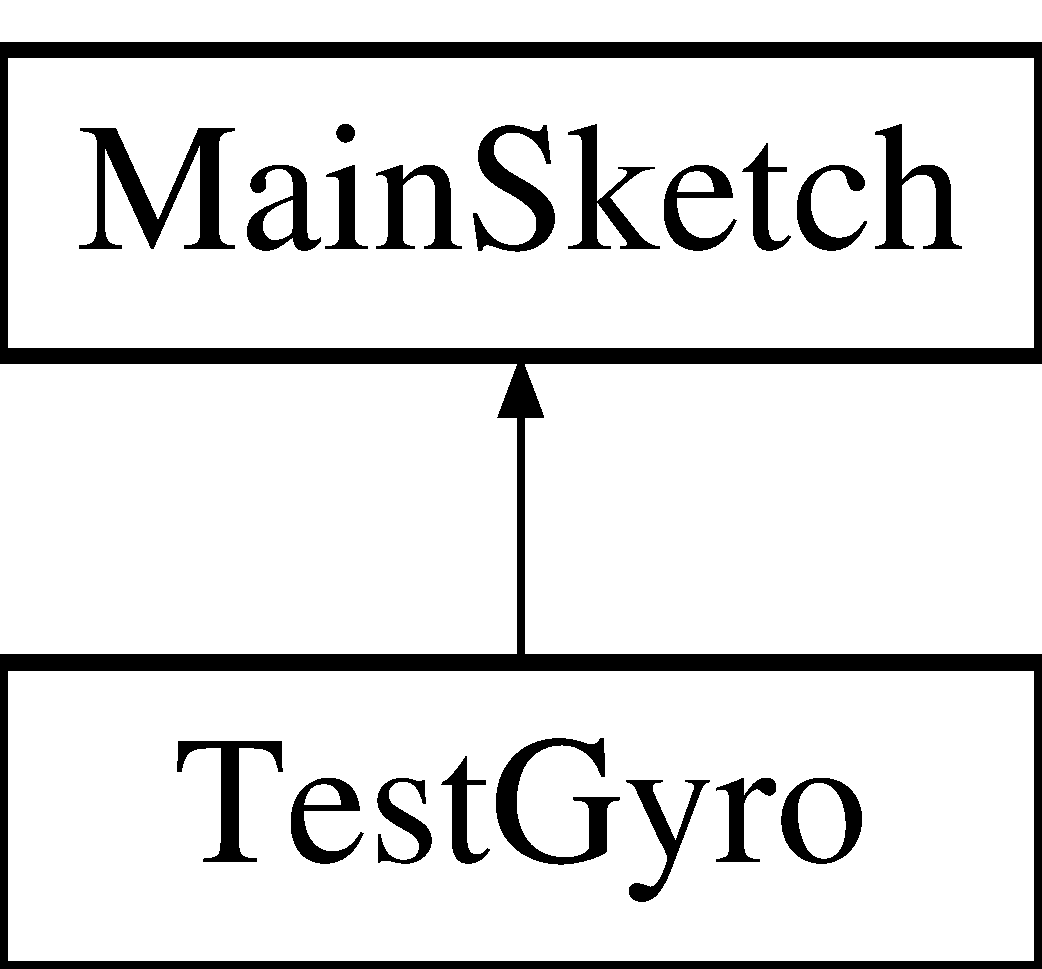
\includegraphics[height=2.000000cm]{classTestGyro}
\end{center}
\end{figure}
\subsection*{Public Member Functions}
\begin{DoxyCompactItemize}
\item 
void \hyperlink{classTestGyro_a22db01127ec2059a00d2c47f07fa6302}{setup} ()
\begin{DoxyCompactList}\small\item\em pure virtual function for setup. Sublcasses must define \end{DoxyCompactList}\item 
void \hyperlink{classTestGyro_a7ae3922dac31681bd2adc7aaf34bf58e}{loop} ()
\begin{DoxyCompactList}\small\item\em pure virtual function for loop. Sublcasses must define \end{DoxyCompactList}\end{DoxyCompactItemize}
\subsection*{Private Attributes}
\begin{DoxyCompactItemize}
\item 
\hyperlink{classGyro}{Gyro} \hyperlink{classTestGyro_a3227ef60350305553a8cd0712aa807bb}{gyro}
\end{DoxyCompactItemize}


\subsection{Detailed Description}


Definition at line 6 of file Test\-Gyro.\-hpp.



\subsection{Member Function Documentation}
\hypertarget{classTestGyro_a7ae3922dac31681bd2adc7aaf34bf58e}{\index{Test\-Gyro@{Test\-Gyro}!loop@{loop}}
\index{loop@{loop}!TestGyro@{Test\-Gyro}}
\subsubsection[{loop}]{\setlength{\rightskip}{0pt plus 5cm}void Test\-Gyro\-::loop (
\begin{DoxyParamCaption}
{}
\end{DoxyParamCaption}
)\hspace{0.3cm}{\ttfamily [virtual]}}}\label{classTestGyro_a7ae3922dac31681bd2adc7aaf34bf58e}


pure virtual function for loop. Sublcasses must define 



Implements \hyperlink{classMainSketch_acd69845de8c794dce73d309f142a6795}{Main\-Sketch}.



Definition at line 7 of file Test\-Gyro.\-cpp.

\hypertarget{classTestGyro_a22db01127ec2059a00d2c47f07fa6302}{\index{Test\-Gyro@{Test\-Gyro}!setup@{setup}}
\index{setup@{setup}!TestGyro@{Test\-Gyro}}
\subsubsection[{setup}]{\setlength{\rightskip}{0pt plus 5cm}void Test\-Gyro\-::setup (
\begin{DoxyParamCaption}
{}
\end{DoxyParamCaption}
)\hspace{0.3cm}{\ttfamily [virtual]}}}\label{classTestGyro_a22db01127ec2059a00d2c47f07fa6302}


pure virtual function for setup. Sublcasses must define 



Implements \hyperlink{classMainSketch_a0708e1eb0ced1063f600f4111df90bf2}{Main\-Sketch}.



Definition at line 3 of file Test\-Gyro.\-cpp.



\subsection{Member Data Documentation}
\hypertarget{classTestGyro_a3227ef60350305553a8cd0712aa807bb}{\index{Test\-Gyro@{Test\-Gyro}!gyro@{gyro}}
\index{gyro@{gyro}!TestGyro@{Test\-Gyro}}
\subsubsection[{gyro}]{\setlength{\rightskip}{0pt plus 5cm}{\bf Gyro} Test\-Gyro\-::gyro\hspace{0.3cm}{\ttfamily [private]}}}\label{classTestGyro_a3227ef60350305553a8cd0712aa807bb}


Definition at line 12 of file Test\-Gyro.\-hpp.



The documentation for this class was generated from the following files\-:\begin{DoxyCompactItemize}
\item 
src/test/\hyperlink{TestGyro_8hpp}{Test\-Gyro.\-hpp}\item 
src/test/\hyperlink{TestGyro_8cpp}{Test\-Gyro.\-cpp}\end{DoxyCompactItemize}

\hypertarget{classTestOdom}{\section{Test\-Odom Class Reference}
\label{classTestOdom}\index{Test\-Odom@{Test\-Odom}}
}


{\ttfamily \#include $<$Test\-Odom.\-hpp$>$}

Inheritance diagram for Test\-Odom\-:\begin{figure}[H]
\begin{center}
\leavevmode
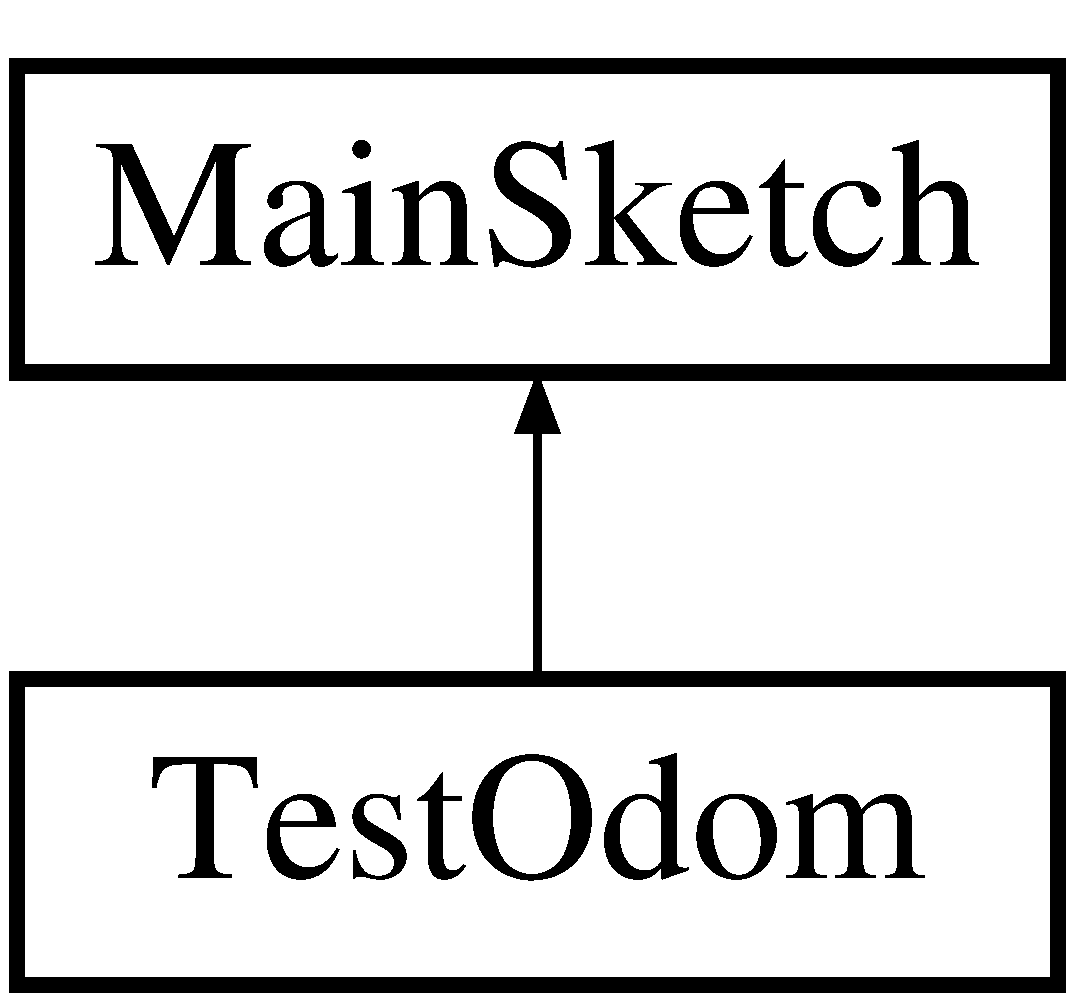
\includegraphics[height=2.000000cm]{classTestOdom}
\end{center}
\end{figure}
\subsection*{Public Member Functions}
\begin{DoxyCompactItemize}
\item 
void \hyperlink{classTestOdom_ac468b764eecd5e27f3d1eb7667810230}{setup} ()
\item 
void \hyperlink{classTestOdom_aa920dd334ddf70f766499f798ca57a8b}{loop} ()
\item 
void \hyperlink{classTestOdom_a27f879657a8c2304e41d5495cf60b809}{avoid\-In\-Front} (int distance)
\end{DoxyCompactItemize}
\subsection*{Private Attributes}
\begin{DoxyCompactItemize}
\item 
\hyperlink{classLidar}{Lidar} \hyperlink{classTestOdom_a4b17e0e5d2294c284a6bc4c3a496b9dd}{lidar}
\item 
\hyperlink{classPIDBase}{P\-I\-D\-Base} \hyperlink{classTestOdom_a185b4bf8f3906701729e77109a22538a}{base}
\item 
int $\ast$ \hyperlink{classTestOdom_a235ba0e8870aec23452d6030efaf8c7e}{distances}
\item 
bool \hyperlink{classTestOdom_ac289c026423da6aec36952f02bc39b4f}{found\-Candle}
\item 
bool \hyperlink{classTestOdom_aacd35fc57d03d28c22cda5c414ae72fb}{considering\-Candle}
\item 
\hyperlink{classCandleDetector}{Candle\-Detector} \hyperlink{classTestOdom_a4ea35bef135d6bf40b9377ae6c38f1d9}{cd}
\item 
int \hyperlink{classTestOdom_a5645cf7c9e70140e5b7b96d3168e8006}{candle\-Angle} = 0
\item 
int \hyperlink{classTestOdom_a64c15d32fcf64aa273cc19f210accd35}{candle\-Distance} = 0
\item 
int \hyperlink{classTestOdom_a336a8f23ac4a1dcc780448bc7ef7f88b}{count} = 0
\end{DoxyCompactItemize}


\subsection{Detailed Description}


Definition at line 7 of file Test\-Odom.\-hpp.



\subsection{Member Function Documentation}
\hypertarget{classTestOdom_a27f879657a8c2304e41d5495cf60b809}{\index{Test\-Odom@{Test\-Odom}!avoid\-In\-Front@{avoid\-In\-Front}}
\index{avoid\-In\-Front@{avoid\-In\-Front}!TestOdom@{Test\-Odom}}
\subsubsection[{avoid\-In\-Front}]{\setlength{\rightskip}{0pt plus 5cm}void Test\-Odom\-::avoid\-In\-Front (
\begin{DoxyParamCaption}
\item[{int}]{distance}
\end{DoxyParamCaption}
)}}\label{classTestOdom_a27f879657a8c2304e41d5495cf60b809}


Definition at line 11 of file Test\-Odom.\-cpp.

\hypertarget{classTestOdom_aa920dd334ddf70f766499f798ca57a8b}{\index{Test\-Odom@{Test\-Odom}!loop@{loop}}
\index{loop@{loop}!TestOdom@{Test\-Odom}}
\subsubsection[{loop}]{\setlength{\rightskip}{0pt plus 5cm}void Test\-Odom\-::loop (
\begin{DoxyParamCaption}
{}
\end{DoxyParamCaption}
)\hspace{0.3cm}{\ttfamily [virtual]}}}\label{classTestOdom_aa920dd334ddf70f766499f798ca57a8b}


Implements \hyperlink{classMainSketch_acd69845de8c794dce73d309f142a6795}{Main\-Sketch}.



Definition at line 20 of file Test\-Odom.\-cpp.

\hypertarget{classTestOdom_ac468b764eecd5e27f3d1eb7667810230}{\index{Test\-Odom@{Test\-Odom}!setup@{setup}}
\index{setup@{setup}!TestOdom@{Test\-Odom}}
\subsubsection[{setup}]{\setlength{\rightskip}{0pt plus 5cm}void Test\-Odom\-::setup (
\begin{DoxyParamCaption}
{}
\end{DoxyParamCaption}
)\hspace{0.3cm}{\ttfamily [virtual]}}}\label{classTestOdom_ac468b764eecd5e27f3d1eb7667810230}


Implements \hyperlink{classMainSketch_a0708e1eb0ced1063f600f4111df90bf2}{Main\-Sketch}.



Definition at line 6 of file Test\-Odom.\-cpp.



\subsection{Member Data Documentation}
\hypertarget{classTestOdom_a185b4bf8f3906701729e77109a22538a}{\index{Test\-Odom@{Test\-Odom}!base@{base}}
\index{base@{base}!TestOdom@{Test\-Odom}}
\subsubsection[{base}]{\setlength{\rightskip}{0pt plus 5cm}{\bf P\-I\-D\-Base} Test\-Odom\-::base\hspace{0.3cm}{\ttfamily [private]}}}\label{classTestOdom_a185b4bf8f3906701729e77109a22538a}


Definition at line 16 of file Test\-Odom.\-hpp.

\hypertarget{classTestOdom_a5645cf7c9e70140e5b7b96d3168e8006}{\index{Test\-Odom@{Test\-Odom}!candle\-Angle@{candle\-Angle}}
\index{candle\-Angle@{candle\-Angle}!TestOdom@{Test\-Odom}}
\subsubsection[{candle\-Angle}]{\setlength{\rightskip}{0pt plus 5cm}int Test\-Odom\-::candle\-Angle = 0\hspace{0.3cm}{\ttfamily [private]}}}\label{classTestOdom_a5645cf7c9e70140e5b7b96d3168e8006}


Definition at line 21 of file Test\-Odom.\-hpp.

\hypertarget{classTestOdom_a64c15d32fcf64aa273cc19f210accd35}{\index{Test\-Odom@{Test\-Odom}!candle\-Distance@{candle\-Distance}}
\index{candle\-Distance@{candle\-Distance}!TestOdom@{Test\-Odom}}
\subsubsection[{candle\-Distance}]{\setlength{\rightskip}{0pt plus 5cm}int Test\-Odom\-::candle\-Distance = 0\hspace{0.3cm}{\ttfamily [private]}}}\label{classTestOdom_a64c15d32fcf64aa273cc19f210accd35}


Definition at line 22 of file Test\-Odom.\-hpp.

\hypertarget{classTestOdom_a4ea35bef135d6bf40b9377ae6c38f1d9}{\index{Test\-Odom@{Test\-Odom}!cd@{cd}}
\index{cd@{cd}!TestOdom@{Test\-Odom}}
\subsubsection[{cd}]{\setlength{\rightskip}{0pt plus 5cm}{\bf Candle\-Detector} Test\-Odom\-::cd\hspace{0.3cm}{\ttfamily [private]}}}\label{classTestOdom_a4ea35bef135d6bf40b9377ae6c38f1d9}


Definition at line 20 of file Test\-Odom.\-hpp.

\hypertarget{classTestOdom_aacd35fc57d03d28c22cda5c414ae72fb}{\index{Test\-Odom@{Test\-Odom}!considering\-Candle@{considering\-Candle}}
\index{considering\-Candle@{considering\-Candle}!TestOdom@{Test\-Odom}}
\subsubsection[{considering\-Candle}]{\setlength{\rightskip}{0pt plus 5cm}bool Test\-Odom\-::considering\-Candle\hspace{0.3cm}{\ttfamily [private]}}}\label{classTestOdom_aacd35fc57d03d28c22cda5c414ae72fb}


Definition at line 18 of file Test\-Odom.\-hpp.

\hypertarget{classTestOdom_a336a8f23ac4a1dcc780448bc7ef7f88b}{\index{Test\-Odom@{Test\-Odom}!count@{count}}
\index{count@{count}!TestOdom@{Test\-Odom}}
\subsubsection[{count}]{\setlength{\rightskip}{0pt plus 5cm}int Test\-Odom\-::count = 0\hspace{0.3cm}{\ttfamily [private]}}}\label{classTestOdom_a336a8f23ac4a1dcc780448bc7ef7f88b}


Definition at line 23 of file Test\-Odom.\-hpp.

\hypertarget{classTestOdom_a235ba0e8870aec23452d6030efaf8c7e}{\index{Test\-Odom@{Test\-Odom}!distances@{distances}}
\index{distances@{distances}!TestOdom@{Test\-Odom}}
\subsubsection[{distances}]{\setlength{\rightskip}{0pt plus 5cm}int$\ast$ Test\-Odom\-::distances\hspace{0.3cm}{\ttfamily [private]}}}\label{classTestOdom_a235ba0e8870aec23452d6030efaf8c7e}


Definition at line 17 of file Test\-Odom.\-hpp.

\hypertarget{classTestOdom_ac289c026423da6aec36952f02bc39b4f}{\index{Test\-Odom@{Test\-Odom}!found\-Candle@{found\-Candle}}
\index{found\-Candle@{found\-Candle}!TestOdom@{Test\-Odom}}
\subsubsection[{found\-Candle}]{\setlength{\rightskip}{0pt plus 5cm}bool Test\-Odom\-::found\-Candle\hspace{0.3cm}{\ttfamily [private]}}}\label{classTestOdom_ac289c026423da6aec36952f02bc39b4f}


Definition at line 18 of file Test\-Odom.\-hpp.

\hypertarget{classTestOdom_a4b17e0e5d2294c284a6bc4c3a496b9dd}{\index{Test\-Odom@{Test\-Odom}!lidar@{lidar}}
\index{lidar@{lidar}!TestOdom@{Test\-Odom}}
\subsubsection[{lidar}]{\setlength{\rightskip}{0pt plus 5cm}{\bf Lidar} Test\-Odom\-::lidar\hspace{0.3cm}{\ttfamily [private]}}}\label{classTestOdom_a4b17e0e5d2294c284a6bc4c3a496b9dd}


Definition at line 15 of file Test\-Odom.\-hpp.



The documentation for this class was generated from the following files\-:\begin{DoxyCompactItemize}
\item 
src/test/\hyperlink{TestOdom_8hpp}{Test\-Odom.\-hpp}\item 
src/test/\hyperlink{TestOdom_8cpp}{Test\-Odom.\-cpp}\end{DoxyCompactItemize}

\hypertarget{classTurn}{\section{Turn Class Reference}
\label{classTurn}\index{Turn@{Turn}}
}


{\ttfamily \#include $<$Turn.\-hpp$>$}

Inheritance diagram for Turn\-:\begin{figure}[H]
\begin{center}
\leavevmode
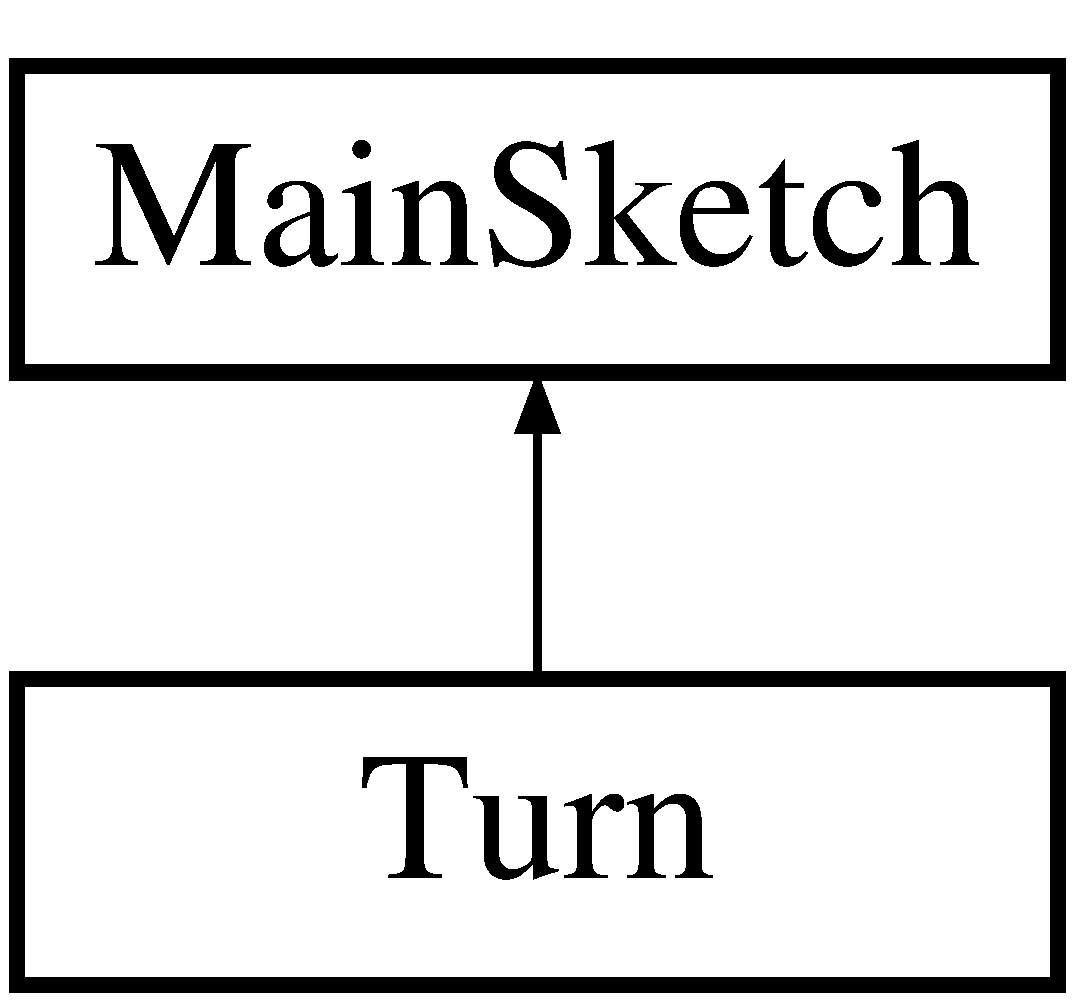
\includegraphics[height=2.000000cm]{classTurn}
\end{center}
\end{figure}
\subsection*{Public Member Functions}
\begin{DoxyCompactItemize}
\item 
void \hyperlink{classTurn_a8fdb6293836d60fb74c5b4d147050373}{setup} ()
\begin{DoxyCompactList}\small\item\em pure virtual function for setup. Sublcasses must define \end{DoxyCompactList}\item 
void \hyperlink{classTurn_ae13f2a047c9ab7e4d4043c568d2fa5e3}{loop} ()
\begin{DoxyCompactList}\small\item\em pure virtual function for loop. Sublcasses must define \end{DoxyCompactList}\end{DoxyCompactItemize}
\subsection*{Private Attributes}
\begin{DoxyCompactItemize}
\item 
float \hyperlink{classTurn_a389aaac2be62ab0a1ab03d729c664e24}{direction}
\item 
long \hyperlink{classTurn_aea10c7359bfbeab45fea812356caae6b}{last\-Update\-Time}
\end{DoxyCompactItemize}


\subsection{Detailed Description}


Definition at line 5 of file Turn.\-hpp.



\subsection{Member Function Documentation}
\hypertarget{classTurn_ae13f2a047c9ab7e4d4043c568d2fa5e3}{\index{Turn@{Turn}!loop@{loop}}
\index{loop@{loop}!Turn@{Turn}}
\subsubsection[{loop}]{\setlength{\rightskip}{0pt plus 5cm}void Turn\-::loop (
\begin{DoxyParamCaption}
{}
\end{DoxyParamCaption}
)\hspace{0.3cm}{\ttfamily [virtual]}}}\label{classTurn_ae13f2a047c9ab7e4d4043c568d2fa5e3}


pure virtual function for loop. Sublcasses must define 



Implements \hyperlink{classMainSketch_acd69845de8c794dce73d309f142a6795}{Main\-Sketch}.



Definition at line 12 of file Turn.\-cpp.

\hypertarget{classTurn_a8fdb6293836d60fb74c5b4d147050373}{\index{Turn@{Turn}!setup@{setup}}
\index{setup@{setup}!Turn@{Turn}}
\subsubsection[{setup}]{\setlength{\rightskip}{0pt plus 5cm}void Turn\-::setup (
\begin{DoxyParamCaption}
{}
\end{DoxyParamCaption}
)\hspace{0.3cm}{\ttfamily [virtual]}}}\label{classTurn_a8fdb6293836d60fb74c5b4d147050373}


pure virtual function for setup. Sublcasses must define 



Implements \hyperlink{classMainSketch_a0708e1eb0ced1063f600f4111df90bf2}{Main\-Sketch}.



Definition at line 6 of file Turn.\-cpp.



\subsection{Member Data Documentation}
\hypertarget{classTurn_a389aaac2be62ab0a1ab03d729c664e24}{\index{Turn@{Turn}!direction@{direction}}
\index{direction@{direction}!Turn@{Turn}}
\subsubsection[{direction}]{\setlength{\rightskip}{0pt plus 5cm}float Turn\-::direction\hspace{0.3cm}{\ttfamily [private]}}}\label{classTurn_a389aaac2be62ab0a1ab03d729c664e24}


Definition at line 11 of file Turn.\-hpp.

\hypertarget{classTurn_aea10c7359bfbeab45fea812356caae6b}{\index{Turn@{Turn}!last\-Update\-Time@{last\-Update\-Time}}
\index{last\-Update\-Time@{last\-Update\-Time}!Turn@{Turn}}
\subsubsection[{last\-Update\-Time}]{\setlength{\rightskip}{0pt plus 5cm}long Turn\-::last\-Update\-Time\hspace{0.3cm}{\ttfamily [private]}}}\label{classTurn_aea10c7359bfbeab45fea812356caae6b}


Definition at line 12 of file Turn.\-hpp.



The documentation for this class was generated from the following files\-:\begin{DoxyCompactItemize}
\item 
src/test/\hyperlink{Turn_8hpp}{Turn.\-hpp}\item 
src/test/\hyperlink{Turn_8cpp}{Turn.\-cpp}\end{DoxyCompactItemize}

\chapter{File Documentation}
\hypertarget{charizard_8hpp}{\section{src/charizard.hpp File Reference}
\label{charizard_8hpp}\index{src/charizard.\-hpp@{src/charizard.\-hpp}}
}
{\ttfamily \#include $<$Liquid\-Crystal.\-h$>$}\\*
{\ttfamily \#include $<$Servo.\-h$>$}\\*
\subsection*{Functions}
\begin{DoxyCompactItemize}
\item 
void \hyperlink{charizard_8hpp_a791f1dbeefa3cf1a8db769cb5b5f68bc}{debug\-Print} (int line, const char $\ast$format,...)
\end{DoxyCompactItemize}
\subsection*{Variables}
\begin{DoxyCompactItemize}
\item 
Liquid\-Crystal \hyperlink{charizard_8hpp_af9292167b3aeb9b70e1ea9b2bbbbc8cd}{Display}
\end{DoxyCompactItemize}


\subsection{Function Documentation}
\hypertarget{charizard_8hpp_a791f1dbeefa3cf1a8db769cb5b5f68bc}{\index{charizard.\-hpp@{charizard.\-hpp}!debug\-Print@{debug\-Print}}
\index{debug\-Print@{debug\-Print}!charizard.hpp@{charizard.\-hpp}}
\subsubsection[{debug\-Print}]{\setlength{\rightskip}{0pt plus 5cm}void debug\-Print (
\begin{DoxyParamCaption}
\item[{int}]{line, }
\item[{const char $\ast$}]{format, }
\item[{}]{...}
\end{DoxyParamCaption}
)}}\label{charizard_8hpp_a791f1dbeefa3cf1a8db769cb5b5f68bc}
debug print to the L\-C\-D 

\subsection{Variable Documentation}
\hypertarget{charizard_8hpp_af9292167b3aeb9b70e1ea9b2bbbbc8cd}{\index{charizard.\-hpp@{charizard.\-hpp}!Display@{Display}}
\index{Display@{Display}!charizard.hpp@{charizard.\-hpp}}
\subsubsection[{Display}]{\setlength{\rightskip}{0pt plus 5cm}Liquid\-Crystal Display}}\label{charizard_8hpp_af9292167b3aeb9b70e1ea9b2bbbbc8cd}
using global extern makes this avaiable to all other files 
\hypertarget{Docs_8h}{\section{src/\-Docs.h File Reference}
\label{Docs_8h}\index{src/\-Docs.\-h@{src/\-Docs.\-h}}
}

\hypertarget{Main_8cpp}{\section{src/\-Main.cpp File Reference}
\label{Main_8cpp}\index{src/\-Main.\-cpp@{src/\-Main.\-cpp}}
}
{\ttfamily \#include \char`\"{}Main.\-hpp\char`\"{}}\\*
{\ttfamily \#include \char`\"{}charizard.\-hpp\char`\"{}}\\*
{\ttfamily \#include \char`\"{}shared/\-Status\-Manager.\-hpp\char`\"{}}\\*
{\ttfamily \#include \char`\"{}Robot.\-hpp\char`\"{}}\\*

\hypertarget{Main_8hpp}{\section{src/\-Main.hpp File Reference}
\label{Main_8hpp}\index{src/\-Main.\-hpp@{src/\-Main.\-hpp}}
}
{\ttfamily \#include \char`\"{}Robot.\-hpp\char`\"{}}\\*
\subsection*{Classes}
\begin{DoxyCompactItemize}
\item 
class \hyperlink{classMain}{Main}
\begin{DoxyCompactList}\small\item\em \hyperlink{classMain}{Main} is the highest level state machine for the robot. \end{DoxyCompactList}\end{DoxyCompactItemize}

\hypertarget{MainSketch_8hpp}{\section{src/\-Main\-Sketch.hpp File Reference}
\label{MainSketch_8hpp}\index{src/\-Main\-Sketch.\-hpp@{src/\-Main\-Sketch.\-hpp}}
}
{\ttfamily \#include \char`\"{}Arduino.\-h\char`\"{}}\\*
\subsection*{Classes}
\begin{DoxyCompactItemize}
\item 
class \hyperlink{classMainSketch}{Main\-Sketch}
\begin{DoxyCompactList}\small\item\em This class is used by charizard. \hyperlink{classMain}{Main} and other test sketches should extend this class and implement setup and loop. \end{DoxyCompactList}\end{DoxyCompactItemize}

\hypertarget{Robot_8cpp}{\section{src/test/\-Robot.cpp File Reference}
\label{Robot_8cpp}\index{src/test/\-Robot.\-cpp@{src/test/\-Robot.\-cpp}}
}
{\ttfamily \#include \char`\"{}Robot.\-hpp\char`\"{}}\\*
{\ttfamily \#include \char`\"{}../main.\-hpp\char`\"{}}\\*
{\ttfamily \#include \char`\"{}Arduino.\-h\char`\"{}}\\*

\hypertarget{Robot_8hpp}{\section{src/\-Robot.hpp File Reference}
\label{Robot_8hpp}\index{src/\-Robot.\-hpp@{src/\-Robot.\-hpp}}
}
{\ttfamily \#include \char`\"{}Main\-Sketch.\-hpp\char`\"{}}\\*
{\ttfamily \#include \char`\"{}shared/\-Lidar.\-hpp\char`\"{}}\\*
{\ttfamily \#include \char`\"{}shared/\-Gyro.\-hpp\char`\"{}}\\*
{\ttfamily \#include \char`\"{}shared/\-Candle\-Detector.\-hpp\char`\"{}}\\*
{\ttfamily \#include \char`\"{}shared/\-Extinguisher.\-hpp\char`\"{}}\\*
{\ttfamily \#include \char`\"{}shared/\-Searcher.\-hpp\char`\"{}}\\*
{\ttfamily \#include \char`\"{}shared/\-P\-I\-D\-Base.\-hpp\char`\"{}}\\*
{\ttfamily \#include \char`\"{}shared/\-Fire\-Finder.\-hpp\char`\"{}}\\*
{\ttfamily \#include \char`\"{}shared/\-Stack.\-hpp\char`\"{}}\\*
{\ttfamily \#include \char`\"{}shared/\-Navigator.\-hpp\char`\"{}}\\*
\subsection*{Classes}
\begin{DoxyCompactItemize}
\item 
class \hyperlink{classRobot}{Robot}
\begin{DoxyCompactList}\small\item\em Contains functions like setting drive P\-I\-Ds, and functions corresponding to states in the \hyperlink{classMain}{Main} state machine. \end{DoxyCompactList}\end{DoxyCompactItemize}

\hypertarget{CandleDetector_8cpp}{\section{src/shared/\-Candle\-Detector.cpp File Reference}
\label{CandleDetector_8cpp}\index{src/shared/\-Candle\-Detector.\-cpp@{src/shared/\-Candle\-Detector.\-cpp}}
}
{\ttfamily \#include $<$Arduino.\-h$>$}\\*
{\ttfamily \#include \char`\"{}Candle\-Detector.\-hpp\char`\"{}}\\*
{\ttfamily \#include $<$stdio.\-h$>$}\\*

\hypertarget{CandleDetector_8hpp}{\section{src/shared/\-Candle\-Detector.hpp File Reference}
\label{CandleDetector_8hpp}\index{src/shared/\-Candle\-Detector.\-hpp@{src/shared/\-Candle\-Detector.\-hpp}}
}
{\ttfamily \#include \char`\"{}Point.\-hpp\char`\"{}}\\*
\subsection*{Classes}
\begin{DoxyCompactItemize}
\item 
class \hyperlink{classCandleDetector}{Candle\-Detector}
\begin{DoxyCompactList}\small\item\em Contains methods for detecting candle and storing its location. \end{DoxyCompactList}\end{DoxyCompactItemize}

\hypertarget{DriveMotor_8cpp}{\section{src/shared/\-Drive\-Motor.cpp File Reference}
\label{DriveMotor_8cpp}\index{src/shared/\-Drive\-Motor.\-cpp@{src/shared/\-Drive\-Motor.\-cpp}}
}
{\ttfamily \#include \char`\"{}Drive\-Motor.\-hpp\char`\"{}}\\*
{\ttfamily \#include $<$stdio.\-h$>$}\\*
{\ttfamily \#include \char`\"{}Arduino.\-h\char`\"{}}\\*

\hypertarget{DriveMotor_8hpp}{\section{src/shared/\-Drive\-Motor.hpp File Reference}
\label{DriveMotor_8hpp}\index{src/shared/\-Drive\-Motor.\-hpp@{src/shared/\-Drive\-Motor.\-hpp}}
}
{\ttfamily \#include $<$Servo.\-h$>$}\\*
\subsection*{Classes}
\begin{DoxyCompactItemize}
\item 
class \hyperlink{classDriveMotor}{Drive\-Motor}
\begin{DoxyCompactList}\small\item\em Basic wrapper around servo that allows -\/100 to 100 speeds instead of 0 to 180. \end{DoxyCompactList}\end{DoxyCompactItemize}
\subsection*{Enumerations}
\begin{DoxyCompactItemize}
\item 
enum \hyperlink{DriveMotor_8hpp_a077d9d13989efa3142086ea83cbb1e68}{Drive\-Direction} \{ \hyperlink{DriveMotor_8hpp_a077d9d13989efa3142086ea83cbb1e68aa26736999186daf8146f809e863712a1}{F\-O\-R\-W\-A\-R\-D}, 
\hyperlink{DriveMotor_8hpp_a077d9d13989efa3142086ea83cbb1e68afed2fca77e454294d6b8bda1bf2c9fd6}{B\-A\-C\-K\-W\-A\-R\-D}, 
\hyperlink{DriveMotor_8hpp_a077d9d13989efa3142086ea83cbb1e68adb45120aafd37a973140edee24708065}{L\-E\-F\-T}, 
\hyperlink{DriveMotor_8hpp_a077d9d13989efa3142086ea83cbb1e68aec8379af7490bb9eaaf579cf17876f38}{R\-I\-G\-H\-T}
 \}
\begin{DoxyCompactList}\small\item\em The basic directions to drive. \end{DoxyCompactList}\end{DoxyCompactItemize}


\subsection{Enumeration Type Documentation}
\hypertarget{DriveMotor_8hpp_a077d9d13989efa3142086ea83cbb1e68}{\index{Drive\-Motor.\-hpp@{Drive\-Motor.\-hpp}!Drive\-Direction@{Drive\-Direction}}
\index{Drive\-Direction@{Drive\-Direction}!DriveMotor.hpp@{Drive\-Motor.\-hpp}}
\subsubsection[{Drive\-Direction}]{\setlength{\rightskip}{0pt plus 5cm}enum {\bf Drive\-Direction}}}\label{DriveMotor_8hpp_a077d9d13989efa3142086ea83cbb1e68}


The basic directions to drive. 

\begin{Desc}
\item[Enumerator]\par
\begin{description}
\index{F\-O\-R\-W\-A\-R\-D@{F\-O\-R\-W\-A\-R\-D}!Drive\-Motor.\-hpp@{Drive\-Motor.\-hpp}}\index{Drive\-Motor.\-hpp@{Drive\-Motor.\-hpp}!F\-O\-R\-W\-A\-R\-D@{F\-O\-R\-W\-A\-R\-D}}\item[{\em 
\hypertarget{DriveMotor_8hpp_a077d9d13989efa3142086ea83cbb1e68aa26736999186daf8146f809e863712a1}{F\-O\-R\-W\-A\-R\-D}\label{DriveMotor_8hpp_a077d9d13989efa3142086ea83cbb1e68aa26736999186daf8146f809e863712a1}
}]\index{B\-A\-C\-K\-W\-A\-R\-D@{B\-A\-C\-K\-W\-A\-R\-D}!Drive\-Motor.\-hpp@{Drive\-Motor.\-hpp}}\index{Drive\-Motor.\-hpp@{Drive\-Motor.\-hpp}!B\-A\-C\-K\-W\-A\-R\-D@{B\-A\-C\-K\-W\-A\-R\-D}}\item[{\em 
\hypertarget{DriveMotor_8hpp_a077d9d13989efa3142086ea83cbb1e68afed2fca77e454294d6b8bda1bf2c9fd6}{B\-A\-C\-K\-W\-A\-R\-D}\label{DriveMotor_8hpp_a077d9d13989efa3142086ea83cbb1e68afed2fca77e454294d6b8bda1bf2c9fd6}
}]\index{L\-E\-F\-T@{L\-E\-F\-T}!Drive\-Motor.\-hpp@{Drive\-Motor.\-hpp}}\index{Drive\-Motor.\-hpp@{Drive\-Motor.\-hpp}!L\-E\-F\-T@{L\-E\-F\-T}}\item[{\em 
\hypertarget{DriveMotor_8hpp_a077d9d13989efa3142086ea83cbb1e68adb45120aafd37a973140edee24708065}{L\-E\-F\-T}\label{DriveMotor_8hpp_a077d9d13989efa3142086ea83cbb1e68adb45120aafd37a973140edee24708065}
}]\index{R\-I\-G\-H\-T@{R\-I\-G\-H\-T}!Drive\-Motor.\-hpp@{Drive\-Motor.\-hpp}}\index{Drive\-Motor.\-hpp@{Drive\-Motor.\-hpp}!R\-I\-G\-H\-T@{R\-I\-G\-H\-T}}\item[{\em 
\hypertarget{DriveMotor_8hpp_a077d9d13989efa3142086ea83cbb1e68aec8379af7490bb9eaaf579cf17876f38}{R\-I\-G\-H\-T}\label{DriveMotor_8hpp_a077d9d13989efa3142086ea83cbb1e68aec8379af7490bb9eaaf579cf17876f38}
}]\end{description}
\end{Desc}


Definition at line 6 of file Drive\-Motor.\-hpp.


\hypertarget{Encoder_8hpp}{\section{src/shared/\-Encoder.hpp File Reference}
\label{Encoder_8hpp}\index{src/shared/\-Encoder.\-hpp@{src/shared/\-Encoder.\-hpp}}
}
{\ttfamily \#include $<$Arduino.\-h$>$}\\*
\subsection*{Classes}
\begin{DoxyCompactItemize}
\item 
class \hyperlink{classEncoder}{Encoder$<$ port1, port2 $>$}
\end{DoxyCompactItemize}

\hypertarget{Extinguisher_8cpp}{\section{src/shared/\-Extinguisher.cpp File Reference}
\label{Extinguisher_8cpp}\index{src/shared/\-Extinguisher.\-cpp@{src/shared/\-Extinguisher.\-cpp}}
}
{\ttfamily \#include \char`\"{}Extinguisher.\-hpp\char`\"{}}\\*
{\ttfamily \#include \char`\"{}../charizard.\-hpp\char`\"{}}\\*
{\ttfamily \#include \char`\"{}../\-Robot.\-hpp\char`\"{}}\\*

\hypertarget{Extinguisher_8hpp}{\section{src/shared/\-Extinguisher.hpp File Reference}
\label{Extinguisher_8hpp}\index{src/shared/\-Extinguisher.\-hpp@{src/shared/\-Extinguisher.\-hpp}}
}
{\ttfamily \#include \char`\"{}Fan.\-hpp\char`\"{}}\\*
\subsection*{Classes}
\begin{DoxyCompactItemize}
\item 
class \hyperlink{classExtinguisher}{Extinguisher}
\begin{DoxyCompactList}\small\item\em Houses the state machine for extinguishing the candle. \hyperlink{classFan}{Fan} is included. \end{DoxyCompactList}\end{DoxyCompactItemize}

\hypertarget{Fan_8cpp}{\section{src/shared/\-Fan.cpp File Reference}
\label{Fan_8cpp}\index{src/shared/\-Fan.\-cpp@{src/shared/\-Fan.\-cpp}}
}
{\ttfamily \#include \char`\"{}Fan.\-hpp\char`\"{}}\\*
{\ttfamily \#include \char`\"{}Arduino.\-h\char`\"{}}\\*

\hypertarget{Fan_8hpp}{\section{src/shared/\-Fan.hpp File Reference}
\label{Fan_8hpp}\index{src/shared/\-Fan.\-hpp@{src/shared/\-Fan.\-hpp}}
}
{\ttfamily \#include $<$Servo.\-h$>$}\\*
\subsection*{Classes}
\begin{DoxyCompactItemize}
\item 
class \hyperlink{classFan}{Fan}
\end{DoxyCompactItemize}

\hypertarget{FireFinder_8cpp}{\section{src/shared/\-Fire\-Finder.cpp File Reference}
\label{FireFinder_8cpp}\index{src/shared/\-Fire\-Finder.\-cpp@{src/shared/\-Fire\-Finder.\-cpp}}
}
{\ttfamily \#include \char`\"{}Fire\-Finder.\-hpp\char`\"{}}\\*
{\ttfamily \#include \char`\"{}Arduino.\-h\char`\"{}}\\*
{\ttfamily \#include $<$math.\-h$>$}\\*
{\ttfamily \#include $<$stdio.\-h$>$}\\*

\hypertarget{FireFinder_8hpp}{\section{src/shared/\-Fire\-Finder.hpp File Reference}
\label{FireFinder_8hpp}\index{src/shared/\-Fire\-Finder.\-hpp@{src/shared/\-Fire\-Finder.\-hpp}}
}
{\ttfamily \#include $<$Servo.\-h$>$}\\*
\subsection*{Classes}
\begin{DoxyCompactItemize}
\item 
class \hyperlink{classFireFinder}{Fire\-Finder}
\end{DoxyCompactItemize}

\hypertarget{Gyro_8cpp}{\section{src/shared/\-Gyro.cpp File Reference}
\label{Gyro_8cpp}\index{src/shared/\-Gyro.\-cpp@{src/shared/\-Gyro.\-cpp}}
}
{\ttfamily \#include \char`\"{}Gyro.\-hpp\char`\"{}}\\*

\hypertarget{Gyro_8hpp}{\section{src/shared/\-Gyro.hpp File Reference}
\label{Gyro_8hpp}\index{src/shared/\-Gyro.\-hpp@{src/shared/\-Gyro.\-hpp}}
}
{\ttfamily \#include $<$L3\-G.\-h$>$}\\*
{\ttfamily \#include $<$Wire.\-h$>$}\\*
\subsection*{Classes}
\begin{DoxyCompactItemize}
\item 
class \hyperlink{classGyro}{Gyro}
\begin{DoxyCompactList}\small\item\em simple wrapper around L3\-G gyro to do the integration \end{DoxyCompactList}\end{DoxyCompactItemize}

\hypertarget{Lidar_8cpp}{\section{src/shared/\-Lidar.cpp File Reference}
\label{Lidar_8cpp}\index{src/shared/\-Lidar.\-cpp@{src/shared/\-Lidar.\-cpp}}
}
{\ttfamily \#include $<$Arduino.\-h$>$}\\*
{\ttfamily \#include \char`\"{}Lidar.\-hpp\char`\"{}}\\*

\hypertarget{Lidar_8hpp}{\section{src/shared/\-Lidar.hpp File Reference}
\label{Lidar_8hpp}\index{src/shared/\-Lidar.\-hpp@{src/shared/\-Lidar.\-hpp}}
}
\subsection*{Classes}
\begin{DoxyCompactItemize}
\item 
class \hyperlink{classLidar}{Lidar}
\end{DoxyCompactItemize}

\hypertarget{Navigator_8cpp}{\section{src/shared/\-Navigator.cpp File Reference}
\label{Navigator_8cpp}\index{src/shared/\-Navigator.\-cpp@{src/shared/\-Navigator.\-cpp}}
}
{\ttfamily \#include \char`\"{}Navigator.\-hpp\char`\"{}}\\*
{\ttfamily \#include \char`\"{}../\-Robot.\-hpp\char`\"{}}\\*

\hypertarget{Navigator_8hpp}{\section{src/shared/\-Navigator.hpp File Reference}
\label{Navigator_8hpp}\index{src/shared/\-Navigator.\-hpp@{src/shared/\-Navigator.\-hpp}}
}
{\ttfamily \#include \char`\"{}Point.\-hpp\char`\"{}}\\*
{\ttfamily \#include \char`\"{}P\-I\-D.\-hpp\char`\"{}}\\*
\subsection*{Classes}
\begin{DoxyCompactItemize}
\item 
class \hyperlink{classNavigator}{Navigator}
\begin{DoxyCompactList}\small\item\em Contains methods for navigating to absolute points on the field. \end{DoxyCompactList}\end{DoxyCompactItemize}

\hypertarget{Odom_8hpp}{\section{src/shared/\-Odom.hpp File Reference}
\label{Odom_8hpp}\index{src/shared/\-Odom.\-hpp@{src/shared/\-Odom.\-hpp}}
}
{\ttfamily \#include \char`\"{}Point.\-hpp\char`\"{}}\\*
{\ttfamily \#include \char`\"{}Encoder.\-hpp\char`\"{}}\\*
{\ttfamily \#include \char`\"{}Gyro.\-hpp\char`\"{}}\\*
{\ttfamily \#include \char`\"{}Status\-Manager.\-hpp\char`\"{}}\\*
{\ttfamily \#include \char`\"{}../charizard.\-hpp\char`\"{}}\\*
\subsection*{Classes}
\begin{DoxyCompactItemize}
\item 
class \hyperlink{classOdom}{Odom$<$ Enc1, Enc2 $>$}
\end{DoxyCompactItemize}

\hypertarget{PID_8cpp}{\section{src/shared/\-P\-I\-D.cpp File Reference}
\label{PID_8cpp}\index{src/shared/\-P\-I\-D.\-cpp@{src/shared/\-P\-I\-D.\-cpp}}
}
{\ttfamily \#include $<$Arduino.\-h$>$}\\*
{\ttfamily \#include \char`\"{}P\-I\-D.\-hpp\char`\"{}}\\*
{\ttfamily \#include \char`\"{}../charizard.\-hpp\char`\"{}}\\*

\hypertarget{PID_8hpp}{\section{src/shared/\-P\-I\-D.hpp File Reference}
\label{PID_8hpp}\index{src/shared/\-P\-I\-D.\-hpp@{src/shared/\-P\-I\-D.\-hpp}}
}
\subsection*{Classes}
\begin{DoxyCompactItemize}
\item 
class \hyperlink{classPID}{P\-I\-D}
\begin{DoxyCompactList}\small\item\em A simple \hyperlink{classPID}{P\-I\-D} controller. \end{DoxyCompactList}\end{DoxyCompactItemize}

\hypertarget{PIDBase_8cpp}{\section{src/shared/\-P\-I\-D\-Base.cpp File Reference}
\label{PIDBase_8cpp}\index{src/shared/\-P\-I\-D\-Base.\-cpp@{src/shared/\-P\-I\-D\-Base.\-cpp}}
}
{\ttfamily \#include \char`\"{}P\-I\-D\-Base.\-hpp\char`\"{}}\\*
{\ttfamily \#include \char`\"{}../main.\-hpp\char`\"{}}\\*

\hypertarget{PIDBase_8hpp}{\section{src/shared/\-P\-I\-D\-Base.hpp File Reference}
\label{PIDBase_8hpp}\index{src/shared/\-P\-I\-D\-Base.\-hpp@{src/shared/\-P\-I\-D\-Base.\-hpp}}
}
{\ttfamily \#include \char`\"{}Encoder.\-hpp\char`\"{}}\\*
{\ttfamily \#include \char`\"{}Odom.\-hpp\char`\"{}}\\*
{\ttfamily \#include \char`\"{}Drive\-Motor.\-hpp\char`\"{}}\\*
{\ttfamily \#include \char`\"{}P\-I\-D.\-hpp\char`\"{}}\\*
\subsection*{Classes}
\begin{DoxyCompactItemize}
\item 
class \hyperlink{classPIDBase}{P\-I\-D\-Base}
\end{DoxyCompactItemize}

\hypertarget{Point_8hpp}{\section{src/shared/\-Point.hpp File Reference}
\label{Point_8hpp}\index{src/shared/\-Point.\-hpp@{src/shared/\-Point.\-hpp}}
}
{\ttfamily \#include $<$math.\-h$>$}\\*
\subsection*{Classes}
\begin{DoxyCompactItemize}
\item 
class \hyperlink{classPoint}{Point$<$ T $>$}
\begin{DoxyCompactList}\small\item\em Represents a point in 2 dimensional space. \end{DoxyCompactList}\end{DoxyCompactItemize}

\hypertarget{Searcher_8cpp}{\section{src/shared/\-Searcher.cpp File Reference}
\label{Searcher_8cpp}\index{src/shared/\-Searcher.\-cpp@{src/shared/\-Searcher.\-cpp}}
}
{\ttfamily \#include \char`\"{}Searcher.\-hpp\char`\"{}}\\*
{\ttfamily \#include \char`\"{}Arduino.\-h\char`\"{}}\\*
{\ttfamily \#include \char`\"{}../test/\-Robot.\-hpp\char`\"{}}\\*

\hypertarget{Searcher_8hpp}{\section{src/shared/\-Searcher.hpp File Reference}
\label{Searcher_8hpp}\index{src/shared/\-Searcher.\-hpp@{src/shared/\-Searcher.\-hpp}}
}
{\ttfamily \#include \char`\"{}Drive\-Motor.\-hpp\char`\"{}}\\*
{\ttfamily \#include \char`\"{}Lidar.\-hpp\char`\"{}}\\*
\subsection*{Classes}
\begin{DoxyCompactItemize}
\item 
class \hyperlink{classSearcher}{Searcher}
\end{DoxyCompactItemize}

\hypertarget{Stack_8hpp}{\section{src/shared/\-Stack.hpp File Reference}
\label{Stack_8hpp}\index{src/shared/\-Stack.\-hpp@{src/shared/\-Stack.\-hpp}}
}
{\ttfamily \#include \char`\"{}Arduino.\-h\char`\"{}}\\*
\subsection*{Classes}
\begin{DoxyCompactItemize}
\item 
class \hyperlink{classStack}{Stack$<$ T, S\-I\-Z\-E $>$}
\end{DoxyCompactItemize}

\hypertarget{StatusManager_8cpp}{\section{src/shared/\-Status\-Manager.cpp File Reference}
\label{StatusManager_8cpp}\index{src/shared/\-Status\-Manager.\-cpp@{src/shared/\-Status\-Manager.\-cpp}}
}
{\ttfamily \#include \char`\"{}Status\-Manager.\-hpp\char`\"{}}\\*

\hypertarget{StatusManager_8hpp}{\section{src/shared/\-Status\-Manager.hpp File Reference}
\label{StatusManager_8hpp}\index{src/shared/\-Status\-Manager.\-hpp@{src/shared/\-Status\-Manager.\-hpp}}
}
{\ttfamily \#include $<$Arduino.\-h$>$}\\*
{\ttfamily \#include \char`\"{}../charizard.\-hpp\char`\"{}}\\*
\subsection*{Classes}
\begin{DoxyCompactItemize}
\item 
class \hyperlink{classStatusManager}{Status\-Manager}
\end{DoxyCompactItemize}

\hypertarget{DriveUntilCandle_8cpp}{\section{src/test/\-Drive\-Until\-Candle.cpp File Reference}
\label{DriveUntilCandle_8cpp}\index{src/test/\-Drive\-Until\-Candle.\-cpp@{src/test/\-Drive\-Until\-Candle.\-cpp}}
}
{\ttfamily \#include \char`\"{}Drive\-Until\-Candle.\-hpp\char`\"{}}\\*
{\ttfamily \#include \char`\"{}../main.\-hpp\char`\"{}}\\*
{\ttfamily \#include $<$math.\-h$>$}\\*

\hypertarget{DriveUntilCandle_8hpp}{\section{src/test/\-Drive\-Until\-Candle.hpp File Reference}
\label{DriveUntilCandle_8hpp}\index{src/test/\-Drive\-Until\-Candle.\-hpp@{src/test/\-Drive\-Until\-Candle.\-hpp}}
}
{\ttfamily \#include \char`\"{}../\-Main\-Sketch.\-hpp\char`\"{}}\\*
{\ttfamily \#include \char`\"{}../shared/\-Lidar.\-hpp\char`\"{}}\\*
{\ttfamily \#include \char`\"{}../shared/\-Candle\-Detector.\-hpp\char`\"{}}\\*
{\ttfamily \#include \char`\"{}../shared/\-P\-I\-D\-Base.\-hpp\char`\"{}}\\*
\subsection*{Classes}
\begin{DoxyCompactItemize}
\item 
class \hyperlink{classDriveUntilCandle}{Drive\-Until\-Candle}
\end{DoxyCompactItemize}

\hypertarget{Height_8cpp}{\section{src/test/\-Height.cpp File Reference}
\label{Height_8cpp}\index{src/test/\-Height.\-cpp@{src/test/\-Height.\-cpp}}
}
{\ttfamily \#include \char`\"{}Height.\-hpp\char`\"{}}\\*
{\ttfamily \#include \char`\"{}Arduino.\-h\char`\"{}}\\*
\subsection*{Variables}
\begin{DoxyCompactItemize}
\item 
long \hyperlink{Height_8cpp_a70a521e476b723cca4aa3de1aa1bc825}{t0}
\item 
const int \hyperlink{Height_8cpp_a4adb49baac164d761359c1af0d2c2bb2}{B\-U\-T\-T\-O\-N\-\_\-\-P\-I\-N} = 29
\end{DoxyCompactItemize}


\subsection{Variable Documentation}
\hypertarget{Height_8cpp_a4adb49baac164d761359c1af0d2c2bb2}{\index{Height.\-cpp@{Height.\-cpp}!B\-U\-T\-T\-O\-N\-\_\-\-P\-I\-N@{B\-U\-T\-T\-O\-N\-\_\-\-P\-I\-N}}
\index{B\-U\-T\-T\-O\-N\-\_\-\-P\-I\-N@{B\-U\-T\-T\-O\-N\-\_\-\-P\-I\-N}!Height.cpp@{Height.\-cpp}}
\subsubsection[{B\-U\-T\-T\-O\-N\-\_\-\-P\-I\-N}]{\setlength{\rightskip}{0pt plus 5cm}const int B\-U\-T\-T\-O\-N\-\_\-\-P\-I\-N = 29}}\label{Height_8cpp_a4adb49baac164d761359c1af0d2c2bb2}


Definition at line 5 of file Height.\-cpp.

\hypertarget{Height_8cpp_a70a521e476b723cca4aa3de1aa1bc825}{\index{Height.\-cpp@{Height.\-cpp}!t0@{t0}}
\index{t0@{t0}!Height.cpp@{Height.\-cpp}}
\subsubsection[{t0}]{\setlength{\rightskip}{0pt plus 5cm}long t0}}\label{Height_8cpp_a70a521e476b723cca4aa3de1aa1bc825}


Definition at line 4 of file Height.\-cpp.


\hypertarget{Height_8hpp}{\section{src/test/\-Height.hpp File Reference}
\label{Height_8hpp}\index{src/test/\-Height.\-hpp@{src/test/\-Height.\-hpp}}
}
{\ttfamily \#include \char`\"{}../\-Main\-Sketch.\-hpp\char`\"{}}\\*
{\ttfamily \#include \char`\"{}../shared/\-Fire\-Finder.\-hpp\char`\"{}}\\*
{\ttfamily \#include \char`\"{}../shared/\-Lidar.\-hpp\char`\"{}}\\*
\subsection*{Classes}
\begin{DoxyCompactItemize}
\item 
class \hyperlink{classHeight}{Height}
\end{DoxyCompactItemize}

\hypertarget{LidarBenchmark_8cpp}{\section{src/test/\-Lidar\-Benchmark.cpp File Reference}
\label{LidarBenchmark_8cpp}\index{src/test/\-Lidar\-Benchmark.\-cpp@{src/test/\-Lidar\-Benchmark.\-cpp}}
}
{\ttfamily \#include \char`\"{}Lidar\-Benchmark.\-hpp\char`\"{}}\\*
\subsection*{Variables}
\begin{DoxyCompactItemize}
\item 
bool \hyperlink{LidarBenchmark_8cpp_aaa928c9a62449f7946da1e32f66c70d2}{on}
\item 
int \hyperlink{LidarBenchmark_8cpp_acb559820d9ca11295b4500f179ef6392}{i} =0
\end{DoxyCompactItemize}


\subsection{Variable Documentation}
\hypertarget{LidarBenchmark_8cpp_acb559820d9ca11295b4500f179ef6392}{\index{Lidar\-Benchmark.\-cpp@{Lidar\-Benchmark.\-cpp}!i@{i}}
\index{i@{i}!LidarBenchmark.cpp@{Lidar\-Benchmark.\-cpp}}
\subsubsection[{i}]{\setlength{\rightskip}{0pt plus 5cm}int i =0}}\label{LidarBenchmark_8cpp_acb559820d9ca11295b4500f179ef6392}


Definition at line 4 of file Lidar\-Benchmark.\-cpp.

\hypertarget{LidarBenchmark_8cpp_aaa928c9a62449f7946da1e32f66c70d2}{\index{Lidar\-Benchmark.\-cpp@{Lidar\-Benchmark.\-cpp}!on@{on}}
\index{on@{on}!LidarBenchmark.cpp@{Lidar\-Benchmark.\-cpp}}
\subsubsection[{on}]{\setlength{\rightskip}{0pt plus 5cm}bool on}}\label{LidarBenchmark_8cpp_aaa928c9a62449f7946da1e32f66c70d2}


Definition at line 3 of file Lidar\-Benchmark.\-cpp.


\hypertarget{LidarBenchmark_8hpp}{\section{src/test/\-Lidar\-Benchmark.hpp File Reference}
\label{LidarBenchmark_8hpp}\index{src/test/\-Lidar\-Benchmark.\-hpp@{src/test/\-Lidar\-Benchmark.\-hpp}}
}
{\ttfamily \#include \char`\"{}../shared/\-Lidar.\-hpp\char`\"{}}\\*
{\ttfamily \#include \char`\"{}../charizard.\-hpp\char`\"{}}\\*
{\ttfamily \#include \char`\"{}../\-Main\-Sketch.\-hpp\char`\"{}}\\*
\subsection*{Classes}
\begin{DoxyCompactItemize}
\item 
class \hyperlink{classLidarBenchmark}{Lidar\-Benchmark}
\end{DoxyCompactItemize}

\hypertarget{LidarDump_8cpp}{\section{src/test/\-Lidar\-Dump.cpp File Reference}
\label{LidarDump_8cpp}\index{src/test/\-Lidar\-Dump.\-cpp@{src/test/\-Lidar\-Dump.\-cpp}}
}
{\ttfamily \#include \char`\"{}Lidar\-Dump.\-hpp\char`\"{}}\\*

\hypertarget{LidarDump_8hpp}{\section{src/test/\-Lidar\-Dump.hpp File Reference}
\label{LidarDump_8hpp}\index{src/test/\-Lidar\-Dump.\-hpp@{src/test/\-Lidar\-Dump.\-hpp}}
}
{\ttfamily \#include \char`\"{}../\-Robot.\-hpp\char`\"{}}\\*
\subsection*{Classes}
\begin{DoxyCompactItemize}
\item 
class \hyperlink{classLidarDump}{Lidar\-Dump}
\end{DoxyCompactItemize}

\hypertarget{PointToCandle_8cpp}{\section{src/test/\-Point\-To\-Candle.cpp File Reference}
\label{PointToCandle_8cpp}\index{src/test/\-Point\-To\-Candle.\-cpp@{src/test/\-Point\-To\-Candle.\-cpp}}
}
{\ttfamily \#include $<$Arduino.\-h$>$}\\*
{\ttfamily \#include \char`\"{}Point\-To\-Candle.\-hpp\char`\"{}}\\*

\hypertarget{PointToCandle_8hpp}{\section{src/test/\-Point\-To\-Candle.hpp File Reference}
\label{PointToCandle_8hpp}\index{src/test/\-Point\-To\-Candle.\-hpp@{src/test/\-Point\-To\-Candle.\-hpp}}
}
{\ttfamily \#include \char`\"{}../main.\-hpp\char`\"{}}\\*
{\ttfamily \#include \char`\"{}Main\-Sketch.\-hpp\char`\"{}}\\*
{\ttfamily \#include \char`\"{}../shared/\-Candle\-Detector.\-hpp\char`\"{}}\\*
{\ttfamily \#include \char`\"{}../shared/\-Lidar.\-hpp\char`\"{}}\\*
{\ttfamily \#include \char`\"{}../shared/\-Drive\-Motor.\-hpp\char`\"{}}\\*
\subsection*{Classes}
\begin{DoxyCompactItemize}
\item 
class \hyperlink{classPointToCandle}{Point\-To\-Candle}
\end{DoxyCompactItemize}

\hypertarget{PrintOdom_8cpp}{\section{src/test/\-Print\-Odom.cpp File Reference}
\label{PrintOdom_8cpp}\index{src/test/\-Print\-Odom.\-cpp@{src/test/\-Print\-Odom.\-cpp}}
}
{\ttfamily \#include \char`\"{}Print\-Odom.\-hpp\char`\"{}}\\*

\hypertarget{PrintOdom_8hpp}{\section{src/test/\-Print\-Odom.hpp File Reference}
\label{PrintOdom_8hpp}\index{src/test/\-Print\-Odom.\-hpp@{src/test/\-Print\-Odom.\-hpp}}
}
{\ttfamily \#include \char`\"{}Main\-Sketch.\-hpp\char`\"{}}\\*
{\ttfamily \#include \char`\"{}../shared/\-Odom.\-hpp\char`\"{}}\\*
{\ttfamily \#include \char`\"{}../shared/\-Point.\-hpp\char`\"{}}\\*
\subsection*{Classes}
\begin{DoxyCompactItemize}
\item 
class \hyperlink{classPrintOdom}{Print\-Odom}
\end{DoxyCompactItemize}

\hypertarget{Search_8cpp}{\section{src/test/\-Search.cpp File Reference}
\label{Search_8cpp}\index{src/test/\-Search.\-cpp@{src/test/\-Search.\-cpp}}
}
{\ttfamily \#include \char`\"{}Search.\-hpp\char`\"{}}\\*
{\ttfamily \#include \char`\"{}Arduino.\-h\char`\"{}}\\*

\hypertarget{Search_8hpp}{\section{src/test/\-Search.hpp File Reference}
\label{Search_8hpp}\index{src/test/\-Search.\-hpp@{src/test/\-Search.\-hpp}}
}
{\ttfamily \#include \char`\"{}Main\-Sketch.\-hpp\char`\"{}}\\*
{\ttfamily \#include \char`\"{}../main.\-hpp\char`\"{}}\\*
{\ttfamily \#include \char`\"{}../shared/\-Drive\-Motor.\-hpp\char`\"{}}\\*
{\ttfamily \#include \char`\"{}../shared/\-Lidar.\-hpp\char`\"{}}\\*
\subsection*{Classes}
\begin{DoxyCompactItemize}
\item 
class \hyperlink{classSearch}{Search}
\end{DoxyCompactItemize}

\hypertarget{TestGyro_8cpp}{\section{src/test/\-Test\-Gyro.cpp File Reference}
\label{TestGyro_8cpp}\index{src/test/\-Test\-Gyro.\-cpp@{src/test/\-Test\-Gyro.\-cpp}}
}
{\ttfamily \#include \char`\"{}Test\-Gyro.\-hpp\char`\"{}}\\*

\hypertarget{TestGyro_8hpp}{\section{src/test/\-Test\-Gyro.hpp File Reference}
\label{TestGyro_8hpp}\index{src/test/\-Test\-Gyro.\-hpp@{src/test/\-Test\-Gyro.\-hpp}}
}
{\ttfamily \#include \char`\"{}../\-Main\-Sketch.\-hpp\char`\"{}}\\*
{\ttfamily \#include \char`\"{}../shared/\-Gyro.\-hpp\char`\"{}}\\*
\subsection*{Classes}
\begin{DoxyCompactItemize}
\item 
class \hyperlink{classTestGyro}{Test\-Gyro}
\end{DoxyCompactItemize}

\hypertarget{TestOdom_8cpp}{\section{src/test/\-Test\-Odom.cpp File Reference}
\label{TestOdom_8cpp}\index{src/test/\-Test\-Odom.\-cpp@{src/test/\-Test\-Odom.\-cpp}}
}
{\ttfamily \#include \char`\"{}Test\-Odom.\-hpp\char`\"{}}\\*
{\ttfamily \#include \char`\"{}../charizard.\-hpp\char`\"{}}\\*
{\ttfamily \#include $<$Memory\-Free.\-h$>$}\\*
{\ttfamily \#include $<$math.\-h$>$}\\*

\hypertarget{TestOdom_8hpp}{\section{src/test/\-Test\-Odom.hpp File Reference}
\label{TestOdom_8hpp}\index{src/test/\-Test\-Odom.\-hpp@{src/test/\-Test\-Odom.\-hpp}}
}
{\ttfamily \#include \char`\"{}Main\-Sketch.\-hpp\char`\"{}}\\*
{\ttfamily \#include \char`\"{}../shared/\-Lidar.\-hpp\char`\"{}}\\*
{\ttfamily \#include \char`\"{}../shared/\-Candle\-Detector.\-hpp\char`\"{}}\\*
{\ttfamily \#include \char`\"{}../shared/\-P\-I\-D\-Base.\-hpp\char`\"{}}\\*
\subsection*{Classes}
\begin{DoxyCompactItemize}
\item 
class \hyperlink{classTestOdom}{Test\-Odom}
\end{DoxyCompactItemize}

\hypertarget{Turn_8cpp}{\section{src/test/\-Turn.cpp File Reference}
\label{Turn_8cpp}\index{src/test/\-Turn.\-cpp@{src/test/\-Turn.\-cpp}}
}
{\ttfamily \#include \char`\"{}Turn.\-hpp\char`\"{}}\\*
{\ttfamily \#include \char`\"{}Arduino.\-h\char`\"{}}\\*
{\ttfamily \#include \char`\"{}../charizard.\-hpp\char`\"{}}\\*
{\ttfamily \#include \char`\"{}../\-Robot.\-hpp\char`\"{}}\\*

\hypertarget{Turn_8hpp}{\section{src/test/\-Turn.hpp File Reference}
\label{Turn_8hpp}\index{src/test/\-Turn.\-hpp@{src/test/\-Turn.\-hpp}}
}
{\ttfamily \#include \char`\"{}../\-Main\-Sketch.\-hpp\char`\"{}}\\*
\subsection*{Classes}
\begin{DoxyCompactItemize}
\item 
class \hyperlink{classTurn}{Turn}
\end{DoxyCompactItemize}

%--- End generated contents ---

% Index
\newpage
\phantomsection
\addcontentsline{toc}{chapter}{Index}
\printindex

\end{document}
